\documentclass[9pt]{beamer}

\usetheme{metropolis}

\usepackage{float}
\usepackage{pgfplots}
\usepackage{pgfplotstable}
%\usepackage{showframe}
\usepackage{subcaption}
\usepackage{tikz}
\usepackage{transparent}
\usepackage{xcolor}

\pgfplotsset{compat=1.18}

\usepgfplotslibrary{fillbetween}
\usepgfplotslibrary{groupplots}

\usetikzlibrary{arrows.meta}
\usetikzlibrary{calc}

\definecolor{ds002424}{HTML}{FF0028}
\definecolor{HBN}{HTML}{FF000E}
\definecolor{ABCD}{HTML}{FF0C00}
\definecolor{QTAB}{HTML}{FF2D00}
\definecolor{PING}{HTML}{FF4800}
\definecolor{ADHD200}{HTML}{FF6800}
\definecolor{PNC}{HTML}{FF8300}
\definecolor{ABIDE II}{HTML}{FFA400}
\definecolor{ds000119}{HTML}{FFBF00}
\definecolor{ABIDE I}{HTML}{FFDF00}
\definecolor{BRAINMINT}{HTML}{FFFA00}
\definecolor{SLIM}{HTML}{E8FF00}
\definecolor{QTIM}{HTML}{C7FF00}
\definecolor{Beijing}{HTML}{ACFF00}
\definecolor{AOMIC-PIOP2}{HTML}{8CFF00}
\definecolor{ds000202}{HTML}{71FF00}
\definecolor{AOMIC-PIOP1}{HTML}{51FF00}
\definecolor{AOMIC-ID1000}{HTML}{36FF00}
\definecolor{CoRR}{HTML}{15FF00}
\definecolor{HCP}{HTML}{00FF05}
\definecolor{FCON1000}{HTML}{00FF20}
\definecolor{ds000171}{HTML}{00FF40}
\definecolor{TOP}{HTML}{00FF5B}
\definecolor{SCZ-Z}{HTML}{00FF7B}
\definecolor{NIMH}{HTML}{00FF96}
\definecolor{NKI-RS}{HTML}{00FFB6}
\definecolor{MPI-LEMON}{HTML}{00FFD1}
\definecolor{ds003592}{HTML}{00FFF1}
\definecolor{ds004302}{HTML}{00F1FF}
\definecolor{ds000222}{HTML}{00D5FF}
\definecolor{SALD}{HTML}{00B5FF}
\definecolor{IXI}{HTML}{009AFF}
\definecolor{DLBS}{HTML}{0079FF}
\definecolor{Cam-CAN}{HTML}{005EFF}
\definecolor{StrokeMRI}{HTML}{003DFF}
\definecolor{PPMI}{HTML}{0022FF}
\definecolor{UKBB}{HTML}{0001FF}
\definecolor{Tao-Wu}{HTML}{1900FF}
\definecolor{ds000245}{HTML}{3400FF}
\definecolor{OASIS3}{HTML}{5500FF}
\definecolor{Demgen}{HTML}{7000FF}
\definecolor{NEUROCON}{HTML}{9000FF}
\definecolor{MIRIAD}{HTML}{AC00FF}
\definecolor{ds004392}{HTML}{CC00FF}
\definecolor{AIBL}{HTML}{E700FF}
\definecolor{ANM}{HTML}{FF00F5}
\definecolor{ADNI}{HTML}{FF00DA}

\definecolor{color0}{rgb}{0.62, 0.004, 0.259}
\definecolor{color1}{rgb}{0.755, 0.154, 0.291}
\definecolor{color2}{rgb}{0.866, 0.29, 0.298}
\definecolor{color3}{rgb}{0.943, 0.406, 0.268}
\definecolor{color4}{rgb}{0.975, 0.557, 0.323}
\definecolor{color5}{rgb}{0.993, 0.709, 0.403}
\definecolor{color6}{rgb}{0.995, 0.832, 0.506}
\definecolor{color7}{rgb}{0.998, 0.926, 0.625}
\definecolor{color8}{rgb}{0.998, 0.999, 0.746}
\definecolor{color9}{rgb}{0.937, 0.975, 0.65}
\definecolor{color10}{rgb}{0.838, 0.935, 0.609}
\definecolor{color11}{rgb}{0.693, 0.876, 0.639}
\definecolor{color12}{rgb}{0.527, 0.811, 0.645}
\definecolor{color13}{rgb}{0.368, 0.725, 0.662}
\definecolor{color14}{rgb}{0.24, 0.582, 0.721}
\definecolor{color15}{rgb}{0.267, 0.441, 0.698}
\definecolor{color16}{rgb}{0.369, 0.31, 0.635}

\definecolor{cases-default}{HTML}{EB5353}
\definecolor{controls-default}{HTML}{0079FF}
\definecolor{healthy-default}{HTML}{36AE7C}

\definecolor{baseline}{HTML}{FAEAB1}
\definecolor{preds}{HTML}{E5BA73}
\definecolor{maps}{HTML}{C58940}

\date{17.06.23}
\title{Explainable artificial intelligence in neuroimaging}
\subtitle{Characterizing individualized neuropathology}
\author{Esten H. Leonardsen}

\def\logoheight{1.2cm}
\def\logosep{0.5cm}

\titlegraphic{
	\centering
	\vspace{7.5cm}
	
\includegraphics[height=\logoheight]{data/norment.png}
	\hspace{\logosep}
	
\includegraphics[height=\logoheight]{data/lifescience.png}
	\hspace{\logosep}
	
\includegraphics[height=\logoheight]{data/lcbc.png}
	\hspace{\logosep}
}


\begin{document}
	\begin{frame}
	 	\maketitle
	\end{frame}

	% XAI: ANNs
	\begin{frame}{Explainable AI}
		\begin{tikzpicture}
			\newcommand{\nodesize}{8pt}
			\newcommand{\hsep}{24pt}
			\newcommand{\vsep}{12pt}

			\newcommand{\arrowwidth}{0.05cm}
			\newcommand{\innerarrow}{{Latex[length=0.1cm, width=0.15cm]}}

			\newcommand{\modellocation}[1]{($ (0, 0) + ####1 $)}

			\colorlet{train-fill}{DLBS}

			\node[circle, inner sep=0pt, fill=none, outer sep=0pt, line width=0pt, draw=none] (n00) at \modellocation{(-3 * \hsep, 0)} {};
			\node[] at (-5.5, 1.5) {};
			\node[] at (5.1, -1.2) {};

			\draw[black, fill=gray!20] (n00.center) --
						 ($ (n00) + (0, 2*\vsep+0.5*\nodesize+2pt) $) --
						 ($ (n00) + (6*\hsep+0.5*\nodesize+2pt, 2*\vsep+0.5*\nodesize+2pt) $) --
						 ($ (n00) + (6*\hsep+0.5*\nodesize+2pt, -2*\vsep-0.5*\nodesize-2pt) $) --
						 ($ (n00) + (0, -2*\vsep-0.5*\nodesize-2pt) $) --
						 (n00.center);


			\node[circle, draw=black, minimum size=\nodesize, inner sep=0pt, fill=gray, outer sep=0pt, line width=0pt, draw=gray] (n10) at \modellocation{(-2 * \hsep, 2 * \vsep)} {};
			\node[circle, minimum size=\nodesize, inner sep=0pt, fill=gray, outer sep=0pt, line width=0pt, draw=gray] (n11) at \modellocation{(-2 * \hsep, 1 * \vsep)} {};
			\node[circle, minimum size=\nodesize, inner sep=0pt, fill=gray, outer sep=0pt, line width=0pt, draw=gray] (n12) at \modellocation{(-2 * \hsep, 0)} {};
			\node[circle, minimum size=\nodesize, inner sep=0pt, fill=gray, outer sep=0pt, line width=0pt, draw=gray] (n13) at \modellocation{(-2 * \hsep, -1 * \vsep)} {};
			\node[circle, minimum size=\nodesize, inner sep=0pt, fill=gray, outer sep=0pt, line width=0pt, draw=gray] (n14) at \modellocation{(-2 * \hsep, -2 * \vsep)} {};

			\node[circle, minimum size=\nodesize, inner sep=0pt, fill=gray, outer sep=0pt, line width=0pt, draw=gray] (n20) at \modellocation{(-1 * \hsep, 1.5 * \vsep)} {};
			\node[circle, minimum size=\nodesize, inner sep=0pt, fill=gray, outer sep=0pt, line width=0pt, draw=gray] (n21) at \modellocation{(-1 * \hsep, 0.5 * \vsep)} {};
			\node[circle, minimum size=\nodesize, inner sep=0pt, fill=gray, outer sep=0pt, line width=0pt, draw=gray] (n22) at \modellocation{(-1 * \hsep, -0.5 * \vsep)} {};
			\node[circle, minimum size=\nodesize, inner sep=0pt, fill=gray, outer sep=0pt, line width=0pt, draw=gray] (n23) at \modellocation{(-1 * \hsep, -1.5 * \vsep)} {};

			\node[circle, minimum size=\nodesize, inner sep=0pt, fill=gray, outer sep=0pt, line width=0pt, draw=gray] (n30) at \modellocation{(0 * \hsep, 1.5 * \vsep)} {};
			\node[circle, minimum size=\nodesize, inner sep=0pt, fill=gray, outer sep=0pt, line width=0pt, draw=gray] (n31) at \modellocation{(0 * \hsep, 0.5 * \vsep)} {};
			\node[circle, minimum size=\nodesize, inner sep=0pt, fill=gray, outer sep=0pt, line width=0pt, draw=gray] (n32) at \modellocation{(0 * \hsep, -0.5 * \vsep)} {};
			\node[circle, minimum size=\nodesize, inner sep=0pt, fill=gray, outer sep=0pt, line width=0pt, draw=gray] (n33) at \modellocation{(0 * \hsep, -1.5 * \vsep)} {};

			\node[circle, minimum size=\nodesize, inner sep=0pt, fill=gray, outer sep=0pt, line width=0pt, draw=gray] (n40) at \modellocation{(1 * \hsep, 1*\vsep)} {};
			\node[circle, minimum size=\nodesize, inner sep=0pt, fill=gray, outer sep=0pt, line width=0pt, draw=gray] (n41) at \modellocation{(1 * \hsep, 0*\vsep)} {};
			\node[circle, minimum size=\nodesize, inner sep=0pt, fill=gray, outer sep=0pt, line width=0pt, draw=gray] (n42) at \modellocation{(1 * \hsep, -1*\vsep)} {};

			\node[circle, minimum size=\nodesize, inner sep=0pt, fill=gray, outer sep=0pt, line width=0pt, draw=gray] (n50) at \modellocation{(2 * \hsep, 1*\vsep)} {};
			\node[circle, minimum size=\nodesize, inner sep=0pt, fill=gray, outer sep=0pt, line width=0pt, draw=gray] (n51) at \modellocation{(2 * \hsep, 0*\vsep)} {};
			\node[circle, minimum size=\nodesize, inner sep=0pt, fill=gray, outer sep=0pt, line width=0pt, draw=gray] (n52) at \modellocation{(2 * \hsep, -1*\vsep)} {};

			\node[circle, minimum size=\nodesize, inner sep=0pt, fill=gray, outer sep=0pt, line width=0pt, draw=gray] (n60) at \modellocation{(3 * \hsep, 0)} {};

			\draw[
				color=gray!70,
				-\innerarrow,
				line width=\arrowwidth
			] (n00) to [out=20,in=200] (n10) {};
			\draw[
				color=gray!70,
				-\innerarrow,
				line width=\arrowwidth
			] (n00) to [out=10,in=190] (n11) {};
			\draw[
				color=gray!70,
				-\innerarrow,
				line width=\arrowwidth
			] (n00) to [out=0,in=180] (n12) {};
			\draw[
				color=gray!70,
				-\innerarrow,
				line width=\arrowwidth
			] (n00) to [out=-10,in=170] (n13) {};
			\draw[
				color=gray!70,
				-\innerarrow,
				line width=\arrowwidth
			] (n00) to [out=-20,in=160] (n14) {};

			\draw[
				color=gray!70,
				-\innerarrow,
				line width=\arrowwidth
			] (n10) to [out=-5,in=175] (n20) {};
			\draw[
				color=gray!70,
				-\innerarrow,
				line width=\arrowwidth
			] (n10) to [out=-15,in=165] (n21) {};
			\draw[
				color=gray!70,
				-\innerarrow,
				line width=\arrowwidth
			] (n10) to [out=-25,in=155] (n22) {};
			\draw[
				color=gray!70,
				-\innerarrow,
				line width=\arrowwidth
			] (n10) to [out=-35,in=145] (n23) {};

			\draw[
				color=gray!70,
				-\innerarrow,
				line width=\arrowwidth
			] (n11) to [out=5,in=185] (n20) {};
			\draw[
				color=gray!70,
				-\innerarrow,
				line width=\arrowwidth
			] (n11) to [out=-5,in=175] (n21) {};
			\draw[
				color=gray!70,
				-\innerarrow,
				line width=\arrowwidth
			] (n11) to [out=-15,in=165] (n22) {};
			\draw[
				color=gray!70,
				-\innerarrow,
				line width=\arrowwidth
			] (n11) to [out=-25,in=155] (n23) {};

			\draw[
				color=gray!70,
				-\innerarrow,
				line width=\arrowwidth
			] (n12) to [out=15,in=195] (n20) {};
			\draw[
				color=gray!70,
				-\innerarrow,
				line width=\arrowwidth
			] (n12) to [out=5,in=185] (n21) {};
			\draw[
				color=gray!70,
				-\innerarrow,
				line width=\arrowwidth
			] (n12) to [out=-5,in=175] (n22) {};
			\draw[
				color=gray!70,
				-\innerarrow,
				line width=\arrowwidth
			] (n12) to [out=-15,in=165] (n23) {};

			\draw[
				color=gray!70,
				-\innerarrow,
				line width=\arrowwidth
			] (n13) to [out=25,in=205] (n20) {};
			\draw[
				color=gray!70,
				-\innerarrow,
				line width=\arrowwidth
			] (n13) to [out=15,in=195] (n21) {};
			\draw[
				color=gray!70,
				-\innerarrow,
				line width=\arrowwidth
			] (n13) to [out=5,in=185] (n22) {};
			\draw[
				color=gray!70,
				-\innerarrow,
				line width=\arrowwidth
			] (n13) to [out=-5,in=175] (n23) {};

			\draw[
				color=gray!70,
				-\innerarrow,
				line width=\arrowwidth
			] (n14) to [out=35,in=215] (n20) {};
			\draw[
				color=gray!70,
				-\innerarrow,
				line width=\arrowwidth
			] (n14) to [out=25,in=205] (n21) {};
			\draw[
				color=gray!70,
				-\innerarrow,
				line width=\arrowwidth
			] (n14) to [out=15,in=195] (n22) {};
			\draw[
				color=gray!70,
				-\innerarrow,
				line width=\arrowwidth
			] (n14) to [out=5,in=185] (n23) {};

			\draw[
				color=gray!70,
				-\innerarrow,
				line width=\arrowwidth
			] (n20) to [out=0,in=180] (n30) {};
			\draw[
				color=gray!70,
				-\innerarrow,
				line width=\arrowwidth
			] (n20) to [out=-10,in=170] (n31) {};
			\draw[
				color=gray!70,
				-\innerarrow,
				line width=\arrowwidth
			] (n20) to [out=-20,in=160] (n32) {};
			\draw[
				color=gray!70,
				-\innerarrow,
				line width=\arrowwidth
			] (n20) to [out=-30,in=150] (n33) {};

			\draw[
				color=gray!70,
				-\innerarrow,
				line width=\arrowwidth
			] (n21) to [out=10,in=190] (n30) {};
			\draw[
				color=gray!70,
				-\innerarrow,
				line width=\arrowwidth
			] (n21) to [out=0,in=180] (n31) {};
			\draw[
				color=gray!70,
				-\innerarrow,
				line width=\arrowwidth
			] (n21) to [out=-10,in=170] (n32) {};
			\draw[
				color=gray!70,
				-\innerarrow,
				line width=\arrowwidth
			] (n21) to [out=-20,in=160] (n33) {};

			\draw[
				color=gray!70,
				-\innerarrow,
				line width=\arrowwidth
			] (n22) to [out=20,in=200] (n30) {};
			\draw[
				color=gray!70,
				-\innerarrow,
				line width=\arrowwidth
			] (n22) to [out=10,in=190] (n31) {};
			\draw[
				color=gray!70,
				-\innerarrow,
				line width=\arrowwidth
			] (n22) to [out=0,in=180] (n32) {};
			\draw[
				color=gray!70,
				-\innerarrow,
				line width=\arrowwidth
			] (n22) to [out=-10,in=170] (n33) {};

			\draw[
				color=gray!70,
				-\innerarrow,
				line width=\arrowwidth
			] (n23) to [out=30,in=210] (n30) {};
			\draw[
				color=gray!70,
				-\innerarrow,
				line width=\arrowwidth
			] (n23) to [out=20,in=200] (n31) {};
			\draw[
				color=gray!70,
				-\innerarrow,
				line width=\arrowwidth
			] (n23) to [out=10,in=190] (n32) {};
			\draw[
				color=gray!70,
				-\innerarrow,
				line width=\arrowwidth
			] (n23) to [out=0,in=180] (n33) {};

			\draw[
				color=gray!70,
				-\innerarrow,
				line width=\arrowwidth
			] (n30) to [out=-5,in=175] (n40) {};
			\draw[
				color=gray!70,
				-\innerarrow,
				line width=\arrowwidth
			] (n30) to [out=-15,in=165] (n41) {};
			\draw[
				color=gray!70,
				-\innerarrow,
				line width=\arrowwidth
			] (n30) to [out=-25,in=155] (n42) {};

			\draw[
				color=gray!70,
				-\innerarrow,
				line width=\arrowwidth
			] (n31) to [out=5,in=185] (n40) {};
			\draw[
				color=gray!70,
				-\innerarrow,
				line width=\arrowwidth
			] (n31) to [out=-5,in=175] (n41) {};
			\draw[
				color=gray!70,
				-\innerarrow,
				line width=\arrowwidth
			] (n31) to [out=-15,in=165] (n42) {};

			\draw[
				color=gray!70,
				-\innerarrow,
				line width=\arrowwidth
			] (n32) to [out=15,in=195] (n40) {};
			\draw[
				color=gray!70,
				-\innerarrow,
				line width=\arrowwidth
			] (n32) to [out=5,in=185] (n41) {};
			\draw[
				color=gray!70,
				-\innerarrow,
				line width=\arrowwidth
			] (n32) to [out=-5,in=175] (n42) {};

			\draw[
				color=gray!70,
				-\innerarrow,
				line width=\arrowwidth
			] (n33) to [out=25,in=205] (n40) {};
			\draw[
				color=gray!70,
				-\innerarrow,
				line width=\arrowwidth
			] (n33) to [out=15,in=195] (n41) {};
			\draw[
				color=gray!70,
				-\innerarrow,
				line width=\arrowwidth
			] (n33) to [out=5,in=185] (n42) {};

			\draw[
				color=gray!70,
				-\innerarrow,
				line width=\arrowwidth
			] (n40) to [out=0,in=180] (n50) {};
			\draw[
				color=gray!70,
				-\innerarrow,
				line width=\arrowwidth
			] (n40) to [out=-10,in=170] (n51) {};
			\draw[
				color=gray!70,
				-\innerarrow,
				line width=\arrowwidth
			] (n40) to [out=-20,in=160] (n52) {};

			\draw[
				color=gray!70,
				-\innerarrow,
				line width=\arrowwidth
			] (n41) to [out=10,in=190] (n50) {};
			\draw[
				color=gray!70,
				-\innerarrow,
				line width=\arrowwidth
			] (n41) to [out=0,in=180] (n51) {};
			\draw[
				color=gray!70,
				-\innerarrow,
				line width=\arrowwidth
			] (n41) to [out=-10,in=170] (n52) {};

			\draw[
				color=gray!70,
				-\innerarrow,
				line width=\arrowwidth
			] (n42) to [out=20,in=200] (n50) {};
			\draw[
				color=gray!70,
				-\innerarrow,
				line width=\arrowwidth
			] (n42) to [out=10,in=190] (n51) {};
			\draw[
				color=gray!70,
				-\innerarrow,
				line width=\arrowwidth
			] (n42) to [out=0,in=180] (n52) {};

			\draw[
				color=gray!70,
				-\innerarrow,
				line width=\arrowwidth,
			] (n50) to [out=-10,in=170] (n60) {};
			\draw[
				color=gray!70,
				-\innerarrow,
				line width=\arrowwidth,
			] (n51) to [out=0,in=180] (n60) {};
			\draw[
				color=gray!70,
				-\innerarrow,
				line width=\arrowwidth,
			] (n52) to [out=10,in=190] (n60) {};


			\node[] at ($ (n30) + (0, \vsep+0.75*\nodesize) $) {Artificial Neural Network};
		\end{tikzpicture}
	\end{frame}

	% XAI: Inputs
	\begin{frame}{Explainable AI}
		\begin{tikzpicture}
			\newcommand{\nodesize}{8pt}
			\newcommand{\hsep}{24pt}
			\newcommand{\vsep}{12pt}

			\newcommand{\arrowwidth}{0.05cm}
			\newcommand{\innerarrow}{{Latex[length=0.1cm, width=0.15cm]}}

			\newcommand{\modellocation}[1]{($ (0, 0) + ####1 $)}

			\colorlet{train-fill}{DLBS}

			\node[circle, inner sep=0pt, fill=none, outer sep=0pt, line width=0pt, draw=none] (n00) at \modellocation{(-3 * \hsep, 0)} {};
			\node[] at (-5.5, 1.5) {};
			\node[] at (5.1, -1.2) {};

			\draw[black, fill=gray!20] (n00.center) --
						 ($ (n00) + (0, 2*\vsep+0.5*\nodesize+2pt) $) --
						 ($ (n00) + (6*\hsep+0.5*\nodesize+2pt, 2*\vsep+0.5*\nodesize+2pt) $) --
						 ($ (n00) + (6*\hsep+0.5*\nodesize+2pt, -2*\vsep-0.5*\nodesize-2pt) $) --
						 ($ (n00) + (0, -2*\vsep-0.5*\nodesize-2pt) $) --
						 (n00.center);


			\node[circle, draw=black, minimum size=\nodesize, inner sep=0pt, fill=train-fill!35, outer sep=0pt, line width=0pt, draw=train-fill!35] (n10) at \modellocation{(-2 * \hsep, 2 * \vsep)} {};
			\node[circle, minimum size=\nodesize, inner sep=0pt, fill=train-fill, outer sep=0pt, line width=0pt, draw=train-fill] (n11) at \modellocation{(-2 * \hsep, 1 * \vsep)} {};
			\node[circle, minimum size=\nodesize, inner sep=0pt, fill=train-fill!15, outer sep=0pt, line width=0pt, draw=train-fill!15] (n12) at \modellocation{(-2 * \hsep, 0)} {};
			\node[circle, minimum size=\nodesize, inner sep=0pt, fill=train-fill!85, outer sep=0pt, line width=0pt, draw=train-fill!85] (n13) at \modellocation{(-2 * \hsep, -1 * \vsep)} {};
			\node[circle, minimum size=\nodesize, inner sep=0pt, fill=train-fill!90, outer sep=0pt, line width=0pt, draw=train-fill!90] (n14) at \modellocation{(-2 * \hsep, -2 * \vsep)} {};

			\node[circle, minimum size=\nodesize, inner sep=0pt, fill=train-fill!55, outer sep=0pt, line width=0pt, draw=train-fill!55] (n20) at \modellocation{(-1 * \hsep, 1.5 * \vsep)} {};
			\node[circle, minimum size=\nodesize, inner sep=0pt, fill=train-fill!20, outer sep=0pt, line width=0pt, draw=train-fill!20] (n21) at \modellocation{(-1 * \hsep, 0.5 * \vsep)} {};
			\node[circle, minimum size=\nodesize, inner sep=0pt, fill=train-fill!90, outer sep=0pt, line width=0pt, draw=train-fill!50] (n22) at \modellocation{(-1 * \hsep, -0.5 * \vsep)} {};
			\node[circle, minimum size=\nodesize, inner sep=0pt, fill=train-fill!35, outer sep=0pt, line width=0pt, draw=train-fill!35] (n23) at \modellocation{(-1 * \hsep, -1.5 * \vsep)} {};

			\node[circle, minimum size=\nodesize, inner sep=0pt, fill=train-fill!95, outer sep=0pt, line width=0pt, draw=train-fill!65] (n30) at \modellocation{(0 * \hsep, 1.5 * \vsep)} {};
			\node[circle, minimum size=\nodesize, inner sep=0pt, fill=train-fill!20, outer sep=0pt, line width=0pt, draw=train-fill!20] (n31) at \modellocation{(0 * \hsep, 0.5 * \vsep)} {};
			\node[circle, minimum size=\nodesize, inner sep=0pt, fill=train-fill!90, outer sep=0pt, line width=0pt, draw=train-fill!90] (n32) at \modellocation{(0 * \hsep, -0.5 * \vsep)} {};
			\node[circle, minimum size=\nodesize, inner sep=0pt, fill=train-fill!80, outer sep=0pt, line width=0pt, draw=train-fill!80] (n33) at \modellocation{(0 * \hsep, -1.5 * \vsep)} {};

			\node[circle, minimum size=\nodesize, inner sep=0pt, fill=train-fill!50, outer sep=0pt, line width=0pt, draw=train-fill!50] (n40) at \modellocation{(1 * \hsep, 1*\vsep)} {};
			\node[circle, minimum size=\nodesize, inner sep=0pt, fill=train-fill!90, outer sep=0pt, line width=0pt, draw=train-fill!70] (n41) at \modellocation{(1 * \hsep, 0*\vsep)} {};
			\node[circle, minimum size=\nodesize, inner sep=0pt, fill=train-fill!70, outer sep=0pt, line width=0pt, draw=train-fill!30] (n42) at \modellocation{(1 * \hsep, -1*\vsep)} {};

			\node[circle, minimum size=\nodesize, inner sep=0pt, fill=train-fill, outer sep=0pt, line width=0pt, draw=train-fill] (n50) at \modellocation{(2 * \hsep, 1*\vsep)} {};
			\node[circle, minimum size=\nodesize, inner sep=0pt, fill=train-fill!70, outer sep=0pt, line width=0pt, draw=train-fill!70] (n51) at \modellocation{(2 * \hsep, 0*\vsep)} {};
			\node[circle, minimum size=\nodesize, inner sep=0pt, fill=train-fill!30, outer sep=0pt, line width=0pt, draw=train-fill!30] (n52) at \modellocation{(2 * \hsep, -1*\vsep)} {};

			\node[circle, minimum size=\nodesize, inner sep=0pt, fill=train-fill!80, outer sep=0pt, line width=0pt, draw=train-fill!65] (n60) at \modellocation{(3 * \hsep, 0)} {};

			\draw[
				color=train-fill!35,
				-\innerarrow,
				line width=\arrowwidth
			] (n00) to [out=20,in=200] (n10) {};
			\draw[
				color=train-fill,
				-\innerarrow,
				line width=\arrowwidth
			] (n00) to [out=10,in=190] (n11) {};
			\draw[
				color=train-fill!15,
				-\innerarrow,
				line width=\arrowwidth
			] (n00) to [out=0,in=180] (n12) {};
			\draw[
				color=train-fill!85,
				-\innerarrow,
				line width=\arrowwidth
			] (n00) to [out=-10,in=170] (n13) {};
			\draw[
				color=train-fill!90,
				-\innerarrow,
				line width=\arrowwidth
			] (n00) to [out=-20,in=160] (n14) {};

			\draw[
				color=train-fill!35,
				-\innerarrow,
				line width=\arrowwidth
			] (n10) to [out=-5,in=175] (n20) {};
			\draw[
				color=train-fill!10,
				-\innerarrow,
				line width=\arrowwidth
			] (n10) to [out=-15,in=165] (n21) {};
			\draw[
				color=train-fill!70,
				-\innerarrow,
				line width=\arrowwidth
			] (n10) to [out=-25,in=155] (n22) {};
			\draw[
				color=train-fill!50,
				-\innerarrow,
				line width=\arrowwidth
			] (n10) to [out=-35,in=145] (n23) {};

			\draw[
				color=train-fill!30,
				-\innerarrow,
				line width=\arrowwidth
			] (n11) to [out=5,in=185] (n20) {};
			\draw[
				color=train-fill!25,
				-\innerarrow,
				line width=\arrowwidth
			] (n11) to [out=-5,in=175] (n21) {};
			\draw[
				color=train-fill!95,
				-\innerarrow,
				line width=\arrowwidth
			] (n11) to [out=-15,in=165] (n22) {};
			\draw[
				color=train-fill!35,
				-\innerarrow,
				line width=\arrowwidth
			] (n11) to [out=-25,in=155] (n23) {};

			\draw[
				color=train-fill!70,
				-\innerarrow,
				line width=\arrowwidth
			] (n12) to [out=15,in=195] (n20) {};
			\draw[
				color=train-fill!20,
				-\innerarrow,
				line width=\arrowwidth
			] (n12) to [out=5,in=185] (n21) {};
			\draw[
				color=train-fill!80,
				-\innerarrow,
				line width=\arrowwidth
			] (n12) to [out=-5,in=175] (n22) {};
			\draw[
				color=train-fill,
				-\innerarrow,
				line width=\arrowwidth
			] (n12) to [out=-15,in=165] (n23) {};

			\draw[
				color=train-fill!40,
				-\innerarrow,
				line width=\arrowwidth
			] (n13) to [out=25,in=205] (n20) {};
			\draw[
				color=train-fill!35,
				-\innerarrow,
				line width=\arrowwidth
			] (n13) to [out=15,in=195] (n21) {};
			\draw[
				color=train-fill!20,
				-\innerarrow,
				line width=\arrowwidth
			] (n13) to [out=5,in=185] (n22) {};
			\draw[
				color=white,
				-\innerarrow,
				line width=\arrowwidth
			] (n13) to [out=-5,in=175] (n23) {};

			\draw[
				color=train-fill!40,
				-\innerarrow,
				line width=\arrowwidth
			] (n14) to [out=35,in=215] (n20) {};
			\draw[
				color=train-fill!85,
				-\innerarrow,
				line width=\arrowwidth
			] (n14) to [out=25,in=205] (n21) {};
			\draw[
				color=train-fill!35,
				-\innerarrow,
				line width=\arrowwidth
			] (n14) to [out=15,in=195] (n22) {};
			\draw[
				color=train-fill,
				-\innerarrow,
				line width=\arrowwidth
			] (n14) to [out=5,in=185] (n23) {};

			\draw[
				color=train-fill!85,
				-\innerarrow,
				line width=\arrowwidth
			] (n20) to [out=0,in=180] (n30) {};
			\draw[
				color=train-fill!50,
				-\innerarrow,
				line width=\arrowwidth
			] (n20) to [out=-10,in=170] (n31) {};
			\draw[
				color=train-fill!75,
				-\innerarrow,
				line width=\arrowwidth
			] (n20) to [out=-20,in=160] (n32) {};
			\draw[
				color=white,
				-\innerarrow,
				line width=\arrowwidth
			] (n20) to [out=-30,in=150] (n33) {};

			\draw[
				color=train-fill,
				-\innerarrow,
				line width=\arrowwidth
			] (n21) to [out=10,in=190] (n30) {};
			\draw[
				color=train-fill!30,
				-\innerarrow,
				line width=\arrowwidth
			] (n21) to [out=0,in=180] (n31) {};
			\draw[
				color=train-fill!25,
				-\innerarrow,
				line width=\arrowwidth
			] (n21) to [out=-10,in=170] (n32) {};
			\draw[
				color=white,
				-\innerarrow,
				line width=\arrowwidth
			] (n21) to [out=-20,in=160] (n33) {};

			\draw[
				color=train-fill!35,
				-\innerarrow,
				line width=\arrowwidth
			] (n22) to [out=20,in=200] (n30) {};
			\draw[
				color=train-fill!95,
				-\innerarrow,
				line width=\arrowwidth
			] (n22) to [out=10,in=190] (n31) {};
			\draw[
				color=train-fill!80,
				-\innerarrow,
				line width=\arrowwidth
			] (n22) to [out=0,in=180] (n32) {};
			\draw[
				color=white,
				-\innerarrow,
				line width=\arrowwidth
			] (n22) to [out=-10,in=170] (n33) {};

			\draw[
				color=train-fill!45,
				-\innerarrow,
				line width=\arrowwidth
			] (n23) to [out=30,in=210] (n30) {};
			\draw[
				color=train-fill!70,
				-\innerarrow,
				line width=\arrowwidth
			] (n23) to [out=20,in=200] (n31) {};
			\draw[
				color=train-fill!10,
				-\innerarrow,
				line width=\arrowwidth
			] (n23) to [out=10,in=190] (n32) {};
			\draw[
				color=train-fill!20,
				-\innerarrow,
				line width=\arrowwidth
			] (n23) to [out=0,in=180] (n33) {};

			\draw[
				color=train-fill!50,
				-\innerarrow,
				line width=\arrowwidth
			] (n30) to [out=-5,in=175] (n40) {};
			\draw[
				color=train-fill!30,
				-\innerarrow,
				line width=\arrowwidth
			] (n30) to [out=-15,in=165] (n41) {};
			\draw[
				color=train-fill,
				-\innerarrow,
				line width=\arrowwidth
			] (n30) to [out=-25,in=155] (n42) {};

			\draw[
				color=train-fill!45,
				-\innerarrow,
				line width=\arrowwidth
			] (n31) to [out=5,in=185] (n40) {};
			\draw[
				color=train-fill!90,
				-\innerarrow,
				line width=\arrowwidth
			] (n31) to [out=-5,in=175] (n41) {};
			\draw[
				color=train-fill!45,
				-\innerarrow,
				line width=\arrowwidth
			] (n31) to [out=-15,in=165] (n42) {};

			\draw[
				color=train-fill!15,
				-\innerarrow,
				line width=\arrowwidth
			] (n32) to [out=15,in=195] (n40) {};
			\draw[
				color=train-fill!70,
				-\innerarrow,
				line width=\arrowwidth
			] (n32) to [out=5,in=185] (n41) {};
			\draw[
				color=train-fill!50,
				-\innerarrow,
				line width=\arrowwidth
			] (n32) to [out=-5,in=175] (n42) {};

			\draw[
				color=train-fill!40,
				-\innerarrow,
				line width=\arrowwidth
			] (n33) to [out=25,in=205] (n40) {};
			\draw[
				color=train-fill!20,
				-\innerarrow,
				line width=\arrowwidth
			] (n33) to [out=15,in=195] (n41) {};
			\draw[
				color=train-fill!90,
				-\innerarrow,
				line width=\arrowwidth
			] (n33) to [out=5,in=185] (n42) {};

			\draw[
				color=train-fill!25,
				-\innerarrow,
				line width=\arrowwidth
			] (n40) to [out=0,in=180] (n50) {};
			\draw[
				color=train-fill!15,
				-\innerarrow,
				line width=\arrowwidth
			] (n40) to [out=-10,in=170] (n51) {};
			\draw[
				color=train-fill,
				-\innerarrow,
				line width=\arrowwidth
			] (n40) to [out=-20,in=160] (n52) {};

			\draw[
				color=train-fill!35,
				-\innerarrow,
				line width=\arrowwidth
			] (n41) to [out=10,in=190] (n50) {};
			\draw[
				color=train-fill!10,
				-\innerarrow,
				line width=\arrowwidth
			] (n41) to [out=0,in=180] (n51) {};
			\draw[
				color=train-fill!90,
				-\innerarrow,
				line width=\arrowwidth
			] (n41) to [out=-10,in=170] (n52) {};

			\draw[
				color=train-fill!50,
				-\innerarrow,
				line width=\arrowwidth
			] (n42) to [out=20,in=200] (n50) {};
			\draw[
				color=train-fill!40,
				-\innerarrow,
				line width=\arrowwidth
			] (n42) to [out=10,in=190] (n51) {};
			\draw[
				color=train-fill!20,
				-\innerarrow,
				line width=\arrowwidth
			] (n42) to [out=0,in=180] (n52) {};

			\draw[
				color=train-fill!80,
				-\innerarrow,
				line width=\arrowwidth,
			] (n50) to [out=-10,in=170] (n60) {};
			\draw[
				color=train-fill!90,
				-\innerarrow,
				line width=\arrowwidth,
			] (n51) to [out=0,in=180] (n60) {};
			\draw[
				color=train-fill!30,
				-\innerarrow,
				line width=\arrowwidth,
			] (n52) to [out=10,in=190] (n60) {};


			\node[] at ($ (n30) + (0, \vsep+0.75*\nodesize) $) {Artificial Neural Network};

			\node[inner sep=0pt, outer sep=0pt, draw=black] (input) at ($ (n00) - (2, 0) $) {
				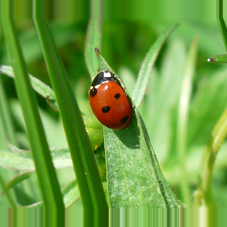
\includegraphics[height=2cm]{data/ladybug.png}
			};

			\newcommand{\outerarrow}{{Latex[length=0.2cm, width=0.3cm]}}
			\draw[-\outerarrow, line width=4pt, draw=gray] (input) to (n00);

		\end{tikzpicture}
	\end{frame}

	% XAI: Prediction
	\begin{frame}{Explainable AI}
		\begin{tikzpicture}
			\newcommand{\nodesize}{8pt}
			\newcommand{\hsep}{24pt}
			\newcommand{\vsep}{12pt}

			\newcommand{\arrowwidth}{0.05cm}
			\newcommand{\innerarrow}{{Latex[length=0.1cm, width=0.15cm]}}

			\newcommand{\modellocation}[1]{($ (0, 0) + ####1 $)}

			\colorlet{train-fill}{DLBS}

			\node[circle, inner sep=0pt, fill=none, outer sep=0pt, line width=0pt, draw=none] (n00) at \modellocation{(-3 * \hsep, 0)} {};
			\node[] at (-5.5, 1.5) {};
			\node[] at (5.1, -1.2) {};

			\draw[black, fill=gray!20] (n00.center) --
						 ($ (n00) + (0, 2*\vsep+0.5*\nodesize+2pt) $) --
						 ($ (n00) + (6*\hsep+0.5*\nodesize+2pt, 2*\vsep+0.5*\nodesize+2pt) $) --
						 ($ (n00) + (6*\hsep+0.5*\nodesize+2pt, -2*\vsep-0.5*\nodesize-2pt) $) --
						 ($ (n00) + (0, -2*\vsep-0.5*\nodesize-2pt) $) --
						 (n00.center);


			\node[circle, draw=black, minimum size=\nodesize, inner sep=0pt, fill=train-fill!35, outer sep=0pt, line width=0pt, draw=train-fill!35] (n10) at \modellocation{(-2 * \hsep, 2 * \vsep)} {};
			\node[circle, minimum size=\nodesize, inner sep=0pt, fill=train-fill, outer sep=0pt, line width=0pt, draw=train-fill] (n11) at \modellocation{(-2 * \hsep, 1 * \vsep)} {};
			\node[circle, minimum size=\nodesize, inner sep=0pt, fill=train-fill!15, outer sep=0pt, line width=0pt, draw=train-fill!15] (n12) at \modellocation{(-2 * \hsep, 0)} {};
			\node[circle, minimum size=\nodesize, inner sep=0pt, fill=train-fill!85, outer sep=0pt, line width=0pt, draw=train-fill!85] (n13) at \modellocation{(-2 * \hsep, -1 * \vsep)} {};
			\node[circle, minimum size=\nodesize, inner sep=0pt, fill=train-fill!90, outer sep=0pt, line width=0pt, draw=train-fill!90] (n14) at \modellocation{(-2 * \hsep, -2 * \vsep)} {};

			\node[circle, minimum size=\nodesize, inner sep=0pt, fill=train-fill!55, outer sep=0pt, line width=0pt, draw=train-fill!55] (n20) at \modellocation{(-1 * \hsep, 1.5 * \vsep)} {};
			\node[circle, minimum size=\nodesize, inner sep=0pt, fill=train-fill!20, outer sep=0pt, line width=0pt, draw=train-fill!20] (n21) at \modellocation{(-1 * \hsep, 0.5 * \vsep)} {};
			\node[circle, minimum size=\nodesize, inner sep=0pt, fill=train-fill!90, outer sep=0pt, line width=0pt, draw=train-fill!50] (n22) at \modellocation{(-1 * \hsep, -0.5 * \vsep)} {};
			\node[circle, minimum size=\nodesize, inner sep=0pt, fill=train-fill!35, outer sep=0pt, line width=0pt, draw=train-fill!35] (n23) at \modellocation{(-1 * \hsep, -1.5 * \vsep)} {};

			\node[circle, minimum size=\nodesize, inner sep=0pt, fill=train-fill!95, outer sep=0pt, line width=0pt, draw=train-fill!65] (n30) at \modellocation{(0 * \hsep, 1.5 * \vsep)} {};
			\node[circle, minimum size=\nodesize, inner sep=0pt, fill=train-fill!20, outer sep=0pt, line width=0pt, draw=train-fill!20] (n31) at \modellocation{(0 * \hsep, 0.5 * \vsep)} {};
			\node[circle, minimum size=\nodesize, inner sep=0pt, fill=train-fill!90, outer sep=0pt, line width=0pt, draw=train-fill!90] (n32) at \modellocation{(0 * \hsep, -0.5 * \vsep)} {};
			\node[circle, minimum size=\nodesize, inner sep=0pt, fill=train-fill!80, outer sep=0pt, line width=0pt, draw=train-fill!80] (n33) at \modellocation{(0 * \hsep, -1.5 * \vsep)} {};

			\node[circle, minimum size=\nodesize, inner sep=0pt, fill=train-fill!50, outer sep=0pt, line width=0pt, draw=train-fill!50] (n40) at \modellocation{(1 * \hsep, 1*\vsep)} {};
			\node[circle, minimum size=\nodesize, inner sep=0pt, fill=train-fill!90, outer sep=0pt, line width=0pt, draw=train-fill!70] (n41) at \modellocation{(1 * \hsep, 0*\vsep)} {};
			\node[circle, minimum size=\nodesize, inner sep=0pt, fill=train-fill!70, outer sep=0pt, line width=0pt, draw=train-fill!30] (n42) at \modellocation{(1 * \hsep, -1*\vsep)} {};

			\node[circle, minimum size=\nodesize, inner sep=0pt, fill=train-fill, outer sep=0pt, line width=0pt, draw=train-fill] (n50) at \modellocation{(2 * \hsep, 1*\vsep)} {};
			\node[circle, minimum size=\nodesize, inner sep=0pt, fill=train-fill!70, outer sep=0pt, line width=0pt, draw=train-fill!70] (n51) at \modellocation{(2 * \hsep, 0*\vsep)} {};
			\node[circle, minimum size=\nodesize, inner sep=0pt, fill=train-fill!30, outer sep=0pt, line width=0pt, draw=train-fill!30] (n52) at \modellocation{(2 * \hsep, -1*\vsep)} {};

			\node[circle, minimum size=\nodesize, inner sep=0pt, fill=train-fill!80, outer sep=0pt, line width=0pt, draw=train-fill!65] (n60) at \modellocation{(3 * \hsep, 0)} {};

			\draw[
				color=train-fill!35,
				-\innerarrow,
				line width=\arrowwidth
			] (n00) to [out=20,in=200] (n10) {};
			\draw[
				color=train-fill,
				-\innerarrow,
				line width=\arrowwidth
			] (n00) to [out=10,in=190] (n11) {};
			\draw[
				color=train-fill!15,
				-\innerarrow,
				line width=\arrowwidth
			] (n00) to [out=0,in=180] (n12) {};
			\draw[
				color=train-fill!85,
				-\innerarrow,
				line width=\arrowwidth
			] (n00) to [out=-10,in=170] (n13) {};
			\draw[
				color=train-fill!90,
				-\innerarrow,
				line width=\arrowwidth
			] (n00) to [out=-20,in=160] (n14) {};

			\draw[
				color=train-fill!35,
				-\innerarrow,
				line width=\arrowwidth
			] (n10) to [out=-5,in=175] (n20) {};
			\draw[
				color=train-fill!10,
				-\innerarrow,
				line width=\arrowwidth
			] (n10) to [out=-15,in=165] (n21) {};
			\draw[
				color=train-fill!70,
				-\innerarrow,
				line width=\arrowwidth
			] (n10) to [out=-25,in=155] (n22) {};
			\draw[
				color=train-fill!50,
				-\innerarrow,
				line width=\arrowwidth
			] (n10) to [out=-35,in=145] (n23) {};

			\draw[
				color=train-fill!30,
				-\innerarrow,
				line width=\arrowwidth
			] (n11) to [out=5,in=185] (n20) {};
			\draw[
				color=train-fill!25,
				-\innerarrow,
				line width=\arrowwidth
			] (n11) to [out=-5,in=175] (n21) {};
			\draw[
				color=train-fill!95,
				-\innerarrow,
				line width=\arrowwidth
			] (n11) to [out=-15,in=165] (n22) {};
			\draw[
				color=train-fill!35,
				-\innerarrow,
				line width=\arrowwidth
			] (n11) to [out=-25,in=155] (n23) {};

			\draw[
				color=train-fill!70,
				-\innerarrow,
				line width=\arrowwidth
			] (n12) to [out=15,in=195] (n20) {};
			\draw[
				color=train-fill!20,
				-\innerarrow,
				line width=\arrowwidth
			] (n12) to [out=5,in=185] (n21) {};
			\draw[
				color=train-fill!80,
				-\innerarrow,
				line width=\arrowwidth
			] (n12) to [out=-5,in=175] (n22) {};
			\draw[
				color=train-fill,
				-\innerarrow,
				line width=\arrowwidth
			] (n12) to [out=-15,in=165] (n23) {};

			\draw[
				color=train-fill!40,
				-\innerarrow,
				line width=\arrowwidth
			] (n13) to [out=25,in=205] (n20) {};
			\draw[
				color=train-fill!35,
				-\innerarrow,
				line width=\arrowwidth
			] (n13) to [out=15,in=195] (n21) {};
			\draw[
				color=train-fill!20,
				-\innerarrow,
				line width=\arrowwidth
			] (n13) to [out=5,in=185] (n22) {};
			\draw[
				color=white,
				-\innerarrow,
				line width=\arrowwidth
			] (n13) to [out=-5,in=175] (n23) {};

			\draw[
				color=train-fill!40,
				-\innerarrow,
				line width=\arrowwidth
			] (n14) to [out=35,in=215] (n20) {};
			\draw[
				color=train-fill!85,
				-\innerarrow,
				line width=\arrowwidth
			] (n14) to [out=25,in=205] (n21) {};
			\draw[
				color=train-fill!35,
				-\innerarrow,
				line width=\arrowwidth
			] (n14) to [out=15,in=195] (n22) {};
			\draw[
				color=train-fill,
				-\innerarrow,
				line width=\arrowwidth
			] (n14) to [out=5,in=185] (n23) {};

			\draw[
				color=train-fill!85,
				-\innerarrow,
				line width=\arrowwidth
			] (n20) to [out=0,in=180] (n30) {};
			\draw[
				color=train-fill!50,
				-\innerarrow,
				line width=\arrowwidth
			] (n20) to [out=-10,in=170] (n31) {};
			\draw[
				color=train-fill!75,
				-\innerarrow,
				line width=\arrowwidth
			] (n20) to [out=-20,in=160] (n32) {};
			\draw[
				color=white,
				-\innerarrow,
				line width=\arrowwidth
			] (n20) to [out=-30,in=150] (n33) {};

			\draw[
				color=train-fill,
				-\innerarrow,
				line width=\arrowwidth
			] (n21) to [out=10,in=190] (n30) {};
			\draw[
				color=train-fill!30,
				-\innerarrow,
				line width=\arrowwidth
			] (n21) to [out=0,in=180] (n31) {};
			\draw[
				color=train-fill!25,
				-\innerarrow,
				line width=\arrowwidth
			] (n21) to [out=-10,in=170] (n32) {};
			\draw[
				color=white,
				-\innerarrow,
				line width=\arrowwidth
			] (n21) to [out=-20,in=160] (n33) {};

			\draw[
				color=train-fill!35,
				-\innerarrow,
				line width=\arrowwidth
			] (n22) to [out=20,in=200] (n30) {};
			\draw[
				color=train-fill!95,
				-\innerarrow,
				line width=\arrowwidth
			] (n22) to [out=10,in=190] (n31) {};
			\draw[
				color=train-fill!80,
				-\innerarrow,
				line width=\arrowwidth
			] (n22) to [out=0,in=180] (n32) {};
			\draw[
				color=white,
				-\innerarrow,
				line width=\arrowwidth
			] (n22) to [out=-10,in=170] (n33) {};

			\draw[
				color=train-fill!45,
				-\innerarrow,
				line width=\arrowwidth
			] (n23) to [out=30,in=210] (n30) {};
			\draw[
				color=train-fill!70,
				-\innerarrow,
				line width=\arrowwidth
			] (n23) to [out=20,in=200] (n31) {};
			\draw[
				color=train-fill!10,
				-\innerarrow,
				line width=\arrowwidth
			] (n23) to [out=10,in=190] (n32) {};
			\draw[
				color=train-fill!20,
				-\innerarrow,
				line width=\arrowwidth
			] (n23) to [out=0,in=180] (n33) {};

			\draw[
				color=train-fill!50,
				-\innerarrow,
				line width=\arrowwidth
			] (n30) to [out=-5,in=175] (n40) {};
			\draw[
				color=train-fill!30,
				-\innerarrow,
				line width=\arrowwidth
			] (n30) to [out=-15,in=165] (n41) {};
			\draw[
				color=train-fill,
				-\innerarrow,
				line width=\arrowwidth
			] (n30) to [out=-25,in=155] (n42) {};

			\draw[
				color=train-fill!45,
				-\innerarrow,
				line width=\arrowwidth
			] (n31) to [out=5,in=185] (n40) {};
			\draw[
				color=train-fill!90,
				-\innerarrow,
				line width=\arrowwidth
			] (n31) to [out=-5,in=175] (n41) {};
			\draw[
				color=train-fill!45,
				-\innerarrow,
				line width=\arrowwidth
			] (n31) to [out=-15,in=165] (n42) {};

			\draw[
				color=train-fill!15,
				-\innerarrow,
				line width=\arrowwidth
			] (n32) to [out=15,in=195] (n40) {};
			\draw[
				color=train-fill!70,
				-\innerarrow,
				line width=\arrowwidth
			] (n32) to [out=5,in=185] (n41) {};
			\draw[
				color=train-fill!50,
				-\innerarrow,
				line width=\arrowwidth
			] (n32) to [out=-5,in=175] (n42) {};

			\draw[
				color=train-fill!40,
				-\innerarrow,
				line width=\arrowwidth
			] (n33) to [out=25,in=205] (n40) {};
			\draw[
				color=train-fill!20,
				-\innerarrow,
				line width=\arrowwidth
			] (n33) to [out=15,in=195] (n41) {};
			\draw[
				color=train-fill!90,
				-\innerarrow,
				line width=\arrowwidth
			] (n33) to [out=5,in=185] (n42) {};

			\draw[
				color=train-fill!25,
				-\innerarrow,
				line width=\arrowwidth
			] (n40) to [out=0,in=180] (n50) {};
			\draw[
				color=train-fill!15,
				-\innerarrow,
				line width=\arrowwidth
			] (n40) to [out=-10,in=170] (n51) {};
			\draw[
				color=train-fill,
				-\innerarrow,
				line width=\arrowwidth
			] (n40) to [out=-20,in=160] (n52) {};

			\draw[
				color=train-fill!35,
				-\innerarrow,
				line width=\arrowwidth
			] (n41) to [out=10,in=190] (n50) {};
			\draw[
				color=train-fill!10,
				-\innerarrow,
				line width=\arrowwidth
			] (n41) to [out=0,in=180] (n51) {};
			\draw[
				color=train-fill!90,
				-\innerarrow,
				line width=\arrowwidth
			] (n41) to [out=-10,in=170] (n52) {};

			\draw[
				color=train-fill!50,
				-\innerarrow,
				line width=\arrowwidth
			] (n42) to [out=20,in=200] (n50) {};
			\draw[
				color=train-fill!40,
				-\innerarrow,
				line width=\arrowwidth
			] (n42) to [out=10,in=190] (n51) {};
			\draw[
				color=train-fill!20,
				-\innerarrow,
				line width=\arrowwidth
			] (n42) to [out=0,in=180] (n52) {};

			\draw[
				color=train-fill!80,
				-\innerarrow,
				line width=\arrowwidth,
			] (n50) to [out=-10,in=170] (n60) {};
			\draw[
				color=train-fill!90,
				-\innerarrow,
				line width=\arrowwidth,
			] (n51) to [out=0,in=180] (n60) {};
			\draw[
				color=train-fill!30,
				-\innerarrow,
				line width=\arrowwidth,
			] (n52) to [out=10,in=190] (n60) {};


			\node[] at ($ (n30) + (0, \vsep+0.75*\nodesize) $) {Artificial Neural Network};

			\node[inner sep=0pt, outer sep=0pt, draw=black] (input) at ($ (n00) - (2, 0) $) {
				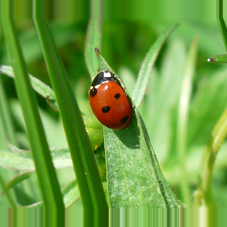
\includegraphics[height=2cm]{data/ladybug.png}
			};
			\node[] (output) at ($ (n60) + (2, 0) $) {
				"ladybug"
			};

			\newcommand{\outerarrow}{{Latex[length=0.2cm, width=0.3cm]}}
			\draw[-\outerarrow, line width=4pt, draw=gray] (input) to (n00);
			\draw[-\outerarrow, line width=4pt, draw=gray] ($ (n60.east) + (0.076, 0) $) to (output);


		\end{tikzpicture}
	\end{frame}

	% XAI: LRP
	\begin{frame}{Explainable AI}
		\begin{tikzpicture}
			\newcommand{\nodesize}{8pt}
			\newcommand{\hsep}{24pt}
			\newcommand{\vsep}{12pt}

			\newcommand{\arrowwidth}{0.05cm}
			\newcommand{\innerarrow}{{Latex[length=0.1cm, width=0.15cm]}}

			\newcommand{\lrplocation}[1]{($ (0, 0) + ####1 $)}

			\colorlet{lrp-fill}{red}
			\colorlet{predict-fill}{blue}

			\node[circle, inner sep=0pt, fill=none, outer sep=0pt, line width=0pt, draw=none] (n00) at \lrplocation{(-3 * \hsep, 0)} {};
			\node[] at (-5.5, 1.5) {};
			\node[] at (5.1, -1.2) {};

			\draw[black, fill=gray!20] (n00.center) --
						 ($ (n00) + (0, 2*\vsep+0.5*\nodesize+2pt) $) --
						 ($ (n00) + (6*\hsep+0.5*\nodesize+2pt, 2*\vsep+0.5*\nodesize+2pt) $) --
						 ($ (n00) + (6*\hsep+0.5*\nodesize+2pt, -2*\vsep-0.5*\nodesize-2pt) $) --
						 ($ (n00) + (0, -2*\vsep-0.5*\nodesize-2pt) $) --
						 (n00.center);


			\node[circle, inner sep=0pt, fill=none, outer sep=0pt, line width=0pt, draw=none] (n00) at \lrplocation{(-3 * \hsep, 0)} {};

			\node[circle, minimum size=\nodesize, inner sep=0pt, fill={rgb:black,5;orange,1}, outer sep=0pt, line width=0pt, draw={rgb:black,5;orange,1}] (n10) at \lrplocation{(-2 * \hsep, 2 * \vsep)} {};
			\node[circle, minimum size=\nodesize, inner sep=0pt, fill={rgb:black,3;red,1}, outer sep=0pt, line width=0pt, draw={rgb:black,3;red,1}] (n11) at \lrplocation{(-2 * \hsep, 1 * \vsep)} {};
			\node[circle, minimum size=\nodesize, inner sep=0pt, fill=yellow, outer sep=0pt, line width=0pt, draw=yellow] (n12) at \lrplocation{(-2 * \hsep, 0)} {};
			\node[circle, minimum size=\nodesize, inner sep=0pt, fill=black, outer sep=0pt, line width=0pt, draw=black] (n13) at \lrplocation{(-2 * \hsep, -1 * \vsep)} {};
			\node[circle, minimum size=\nodesize, inner sep=0pt, fill=red, outer sep=0pt, line width=0pt, draw=red] (n14) at \lrplocation{(-2 * \hsep, -2 * \vsep)} {};

			\node[circle, minimum size=\nodesize, inner sep=0pt, fill={rgb:black,5;white,2;orange,1}, outer sep=0pt, line width=0pt, draw={rgb:black,5;white,2;orange,1}] (n20) at \lrplocation{(-1 * \hsep, 1.5 * \vsep)} {};
			\node[circle, minimum size=\nodesize, inner sep=0pt, fill={rgb:red,10;yellow,6}, outer sep=0pt, line width=0pt, draw={rgb:red,10;yellow,4}] (n21) at \lrplocation{(-1 * \hsep, 0.5 * \vsep)} {};
			\node[circle, minimum size=\nodesize, inner sep=0pt, fill={rgb:red,10;yellow,1}, outer sep=0pt, line width=0pt, draw={rgb:red,10;yellow,1}] (n22) at \lrplocation{(-1 * \hsep, -0.5 * \vsep)} {};
			\node[circle, minimum size=\nodesize, inner sep=0pt, fill={rgb:black,10;red,2}, outer sep=0pt, line width=0pt, draw={rgb:black,10;red,2}] (n23) at \lrplocation{(-1 * \hsep, -1.5 * \vsep)} {};

			\node[circle, minimum size=\nodesize, inner sep=0pt, fill={rgb:red,3;orange,2}, outer sep=0pt, line width=0pt, draw={rgb:red,3;orange,1}] (n30) at \lrplocation{(0 * \hsep, 1.5 * \vsep)} {};
			\node[circle, minimum size=\nodesize, inner sep=0pt, fill={rgb:yellow,3;orange,1}, outer sep=0pt, line width=0pt, draw={rgb:yellow,3;orange,1}] (n31) at \lrplocation{(0 * \hsep, 0.5 * \vsep)} {};
			\node[circle, minimum size=\nodesize, inner sep=0pt, fill={rgb:black,10;white,5;red,1}, outer sep=0pt, line width=0pt, draw={rgb:black,10;white,5;red,1}] (n32) at \lrplocation{(0 * \hsep, -0.5 * \vsep)} {};
			\node[circle, minimum size=\nodesize, inner sep=0pt, fill={rgb:gray,5;red,1}, outer sep=0pt, line width=0pt, draw={rgb:gray,5;red,1}] (n33) at \lrplocation{(0 * \hsep, -1.5 * \vsep)} {};

			\node[circle, minimum size=\nodesize, inner sep=0pt, fill={rgb:yellow,10;orange,1}, outer sep=0pt, line width=0pt, draw={rgb:yellow,10;orange,1}] (n40) at \lrplocation{(1 * \hsep, 1*\vsep)} {};
			\node[circle, minimum size=\nodesize, inner sep=0pt, fill={rgb:red,1}, outer sep=0pt, line width=0pt, draw={rgb:red,1}] (n41) at \lrplocation{(1 * \hsep, 0*\vsep)} {};
			\node[circle, minimum size=\nodesize, inner sep=0pt, fill={rgb:black,10;white,15;red,2}, outer sep=0pt, line width=0pt, draw={rgb:black,10;white,15;red,2}] (n42) at \lrplocation{(1 * \hsep, -1*\vsep)} {};

			\node[circle, minimum size=\nodesize, inner sep=0pt, fill={rgb:red,5;black,1;yellow,2}, outer sep=0pt, line width=0pt, draw={rgb:red,5;black,1;yellow,2}] (n50) at \lrplocation{(2 * \hsep, 1*\vsep)} {};
			\node[circle, minimum size=\nodesize, inner sep=0pt, fill={rgb:gray,5;red,1}, outer sep=0pt, line width=0pt, draw={rgb:gray,5;red,1}] (n51) at \lrplocation{(2 * \hsep, 0*\vsep)} {};
			\node[circle, minimum size=\nodesize, inner sep=0pt, fill={rgb:yellow,5;orange,1}, outer sep=0pt, line width=0pt, draw={rgb:yellow,5;orange,1}] (n52) at \lrplocation{(2 * \hsep, -1*\vsep)} {};

			\node[circle, minimum size=\nodesize, inner sep=0pt, fill={rgb:orange,7;yellow,4;black,1}, outer sep=0pt, line width=0pt, draw={rgb:orange,7;yellow,4;black,1}] (n60) at \lrplocation{(3 * \hsep, 0)} {};

			\draw[
				color={rgb:black,5;orange,1},
				\innerarrow-,
				line width=\arrowwidth
			] (n00) to [out=20,in=200] (n10) {};
			\draw[
				color={rgb:black,3;red,1},
				\innerarrow-,
				line width=\arrowwidth
			] (n00) to [out=10,in=190] (n11) {};
			\draw[
				color=yellow,
				\innerarrow-,
				line width=\arrowwidth
			] (n00) to [out=0,in=180] (n12) {};
			\draw[
				color=black,
				\innerarrow-,
				line width=\arrowwidth
			] (n00) to [out=-10,in=170] (n13) {};
			\draw[
				color=red,
				\innerarrow-,
				line width=\arrowwidth
			] (n00) to [out=-20,in=160] (n14) {};

			\draw[
				color={rgb:black,5;white,1;orange,1},
				\innerarrow-,
				line width=\arrowwidth
			] (n10) to [out=-5,in=175] (n20) {};
			\draw[
				color={rgb:black,3;orange,1},
				\innerarrow-,
				line width=\arrowwidth
			] (n10) to [out=-15,in=165] (n21) {};
			\draw[
				color={rgb:black,4;red,2;yellow,1},
				\innerarrow-,
				line width=\arrowwidth
			] (n10) to [out=-25,in=155] (n22) {};
			\draw[
				color={rgb:black,3;red,1},
				\innerarrow-,
				line width=\arrowwidth
			] (n10) to [out=-35,in=145] (n23) {};

			\draw[
				color={rgb:black,10;orange,2},
				\innerarrow-,
				line width=\arrowwidth
			] (n11) to [out=5,in=185] (n20) {};
			\draw[
				color={rgb:black,3;orange,1},
				\innerarrow-,
				line width=\arrowwidth
			] (n11) to [out=-5,in=175] (n21) {};
			\draw[
				color={rgb:black,3;red,1},
				\innerarrow-,
				line width=\arrowwidth
			] (n11) to [out=-15,in=165] (n22) {};
			\draw[
				color={rgb:black,10;red,1},
				\innerarrow-,
				line width=\arrowwidth
			] (n11) to [out=-25,in=155] (n23) {};

			\draw[
				color={rgb:black,5;orange,3},
				\innerarrow-,
				line width=\arrowwidth
			] (n12) to [out=15,in=195] (n20) {};
			\draw[
				color={rgb:red,3;yellow,5},
				\innerarrow-,
				line width=\arrowwidth
			] (n12) to [out=5,in=185] (n21) {};
			\draw[
				color={rgb:red,5;yellow,3},
				\innerarrow-,
				line width=\arrowwidth
			] (n12) to [out=-5,in=175] (n22) {};
			\draw[
				color={rgb:black,5;orange,2},
				\innerarrow-,
				line width=\arrowwidth
			] (n12) to [out=-15,in=165] (n23) {};

			\draw[
				color={rgb:black,5;red,1},
				\innerarrow-,
				line width=\arrowwidth
			] (n13) to [out=25,in=205] (n20) {};
			\draw[
				color={rgb:black,5;orange,2},
				\innerarrow-,
				line width=\arrowwidth
			] (n13) to [out=15,in=195] (n21) {};
			\draw[
				color={rgb:black,5;red,3},
				\innerarrow-,
				line width=\arrowwidth
			] (n13) to [out=5,in=185] (n22) {};
			\draw[
				color=black,
				\innerarrow-,
				line width=\arrowwidth
			] (n13) to [out=-5,in=175] (n23) {};

			\draw[
				color={rgb:black,5;orange,2},
				\innerarrow-,
				line width=\arrowwidth
			] (n14) to [out=35,in=215] (n20) {};
			\draw[
				color={rgb:red,3;orange,1},
				\innerarrow-,
				line width=\arrowwidth
			] (n14) to [out=25,in=205] (n21) {};
			\draw[
				color={rgb:red,5;yellow,2},
				\innerarrow-,
				line width=\arrowwidth
			] (n14) to [out=15,in=195] (n22) {};
			\draw[
				color={rgb:black,5;red,3},
				\innerarrow-,
				line width=\arrowwidth
			] (n14) to [out=5,in=185] (n23) {};

			\draw[
				color={rgb:black,1;red,1},
				\innerarrow-,
				line width=\arrowwidth
			] (n20) to [out=0,in=180] (n30) {};
			\draw[
				color={rgb:black,3;orange,1},
				\innerarrow-,
				line width=\arrowwidth
			] (n20) to [out=-10,in=170] (n31) {};
			\draw[
				color={rgb:black,10;red,1},
				\innerarrow-,
				line width=\arrowwidth
			] (n20) to [out=-20,in=160] (n32) {};
			\draw[
				color={rgb:black,5;red,1},
				\innerarrow-,
				line width=\arrowwidth
			] (n20) to [out=-30,in=150] (n33) {};

			\draw[
				color={rgb:orange,5;red,2},
				\innerarrow-,
				line width=\arrowwidth
			] (n21) to [out=10,in=190] (n30) {};
			\draw[
				color={rgb:yellow,10;orange,4},
				\innerarrow-,
				line width=\arrowwidth
			] (n21) to [out=0,in=180] (n31) {};
			\draw[
				color={rgb:black,2;red,1},
				\innerarrow-,
				line width=\arrowwidth
			] (n21) to [out=-10,in=170] (n32) {};
			\draw[
				color={rgb:black,1;orange,2;red,1},
				\innerarrow-,
				line width=\arrowwidth
			] (n21) to [out=-20,in=160] (n33) {};

			\draw[
				color={rgb:red,2;orange,1},
				\innerarrow-,
				line width=\arrowwidth
			] (n22) to [out=20,in=200] (n30) {};
			\draw[
				color={rgb:yellow,2;orange,1},
				\innerarrow-,
				line width=\arrowwidth
			] (n22) to [out=10,in=190] (n31) {};
			\draw[
				color={rgb:black,2;red,2},
				\innerarrow-,
				line width=\arrowwidth
			] (n22) to [out=0,in=180] (n32) {};
			\draw[
				color={rgb:black,2;orange,1},
				\innerarrow-,
				line width=\arrowwidth
			] (n22) to [out=-10,in=170] (n33) {};

			\draw[
				color={rgb:black,4;red,2},
				\innerarrow-,
				line width=\arrowwidth
			] (n23) to [out=30,in=210] (n30) {};
			\draw[
				color={rgb:orange,2;black,1},
				\innerarrow-,
				line width=\arrowwidth
			] (n23) to [out=20,in=200] (n31) {};
			\draw[
				color={rgb:black,5;orange,1},
				\innerarrow-,
				line width=\arrowwidth
			] (n23) to [out=10,in=190] (n32) {};
			\draw[
				color={rgb:black,5;red,2},
				\innerarrow-,
				line width=\arrowwidth
			] (n23) to [out=0,in=180] (n33) {};

			\draw[
				color={rgb:orange,3;red,1},
				\innerarrow-,
				line width=\arrowwidth
			] (n30) to [out=-5,in=175] (n40) {};
			\draw[
				color={rgb:gray,1;orange,1;red,2},
				\innerarrow-,
				line width=\arrowwidth
			] (n30) to [out=-15,in=165] (n41) {};
			\draw[
				color={rgb:orange,2;black,2;white,1},
				\innerarrow-,
				line width=\arrowwidth
			] (n30) to [out=-25,in=155] (n42) {};

			\draw[
				color={rgb:yellow,5;orange,1},
				\innerarrow-,
				line width=\arrowwidth
			] (n31) to [out=5,in=185] (n40) {};
			\draw[
				color={rgb:red,3;orange,1},
				\innerarrow-,
				line width=\arrowwidth
			] (n31) to [out=-5,in=175] (n41) {};
			\draw[
				color={rgb:gray,1;red,2},
				\innerarrow-,
				line width=\arrowwidth
			] (n31) to [out=-15,in=165] (n42) {};

			\draw[
				color={rgb:gray,3;orange,1},
				\innerarrow-,
				line width=\arrowwidth
			] (n32) to [out=15,in=195] (n40) {};
			\draw[
				color={rgb:gray,1;red,1},
				\innerarrow-,
				line width=\arrowwidth
			] (n32) to [out=5,in=185] (n41) {};
			\draw[
				color={rgb:gray,1},
				\innerarrow-,
				line width=\arrowwidth
			] (n32) to [out=-5,in=175] (n42) {};

			\draw[
				color={rgb:gray,2;orange,3},
				\innerarrow-,
				line width=\arrowwidth
			] (n33) to [out=25,in=205] (n40) {};
			\draw[
				color={rgb:gray,1;orange,1},
				\innerarrow-,
				line width=\arrowwidth
			] (n33) to [out=15,in=195] (n41) {};
			\draw[
				color={rgb:gray,3;red,1},
				\innerarrow-,
				line width=\arrowwidth
			] (n33) to [out=5,in=185] (n42) {};

			\draw[
				color={rgb:red,3;yellow,1},
				\innerarrow-,
				line width=\arrowwidth
			] (n40) to [out=0,in=180] (n50) {};
			\draw[
				color={rgb:gray,2;orange,1},
				\innerarrow-,
				line width=\arrowwidth
			] (n40) to [out=-10,in=170] (n51) {};
			\draw[
				color={rgb:yellow,10;orange,1},
				\innerarrow-,
				line width=\arrowwidth
			] (n40) to [out=-20,in=160] (n52) {};

			\draw[
				color={rgb:red,5;black,1;yellow,2},
				\innerarrow-,
				line width=\arrowwidth
			] (n41) to [out=10,in=190] (n50) {};
			\draw[
				color={rgb:gray,7;orange,3},
				\innerarrow-,
				line width=\arrowwidth
			] (n41) to [out=0,in=180] (n51) {};
			\draw[
				color={rgb:yellow,1;orange,2},
				\innerarrow-,
				line width=\arrowwidth
			] (n41) to [out=-10,in=170] (n52) {};

			\draw[
				color={rgb:gray,7;orange,2},
				\innerarrow-,
				line width=\arrowwidth
			] (n42) to [out=20,in=200] (n50) {};
			\draw[
				color={rgb:gray,5;red,1},
				\innerarrow-,
				line width=\arrowwidth
			] (n42) to [out=10,in=190] (n51) {};
			\draw[
				color={rgb:gray,5;red,1;black,2},
				\innerarrow-,
				line width=\arrowwidth
			] (n42) to [out=0,in=180] (n52) {};

			\draw[
				color={rgb:red,5;black,1;yellow,2},
				\innerarrow-,
				line width=\arrowwidth
			] (n50) to [out=-10,in=170] (n60) {};
			\draw[
				color={rgb:gray,5;red,1},
				\innerarrow-,
				line width=\arrowwidth
			] (n51) to [out=0,in=180] (n60) {};
			\draw[
				color={rgb:yellow,5;orange,1},
				\innerarrow-,
				line width=\arrowwidth
			] (n52) to [out=10,in=190] (n60) {};


			\node[] at ($ (n30) + (0, \vsep+0.75*\nodesize) $) {Artificial Neural Network};

			\node[inner sep=0pt, outer sep=0pt, draw=black] (input) at ($ (n00) - (2, 0) $) {
				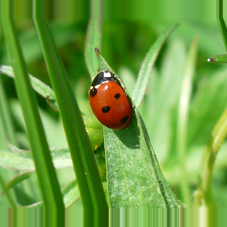
\includegraphics[height=2cm]{data/ladybug.png}
			};
			\node[] (output) at ($ (n60) + (2, 0) $) {
				"ladybug"
			};

			\newcommand{\outerarrow}{{Latex[length=0.2cm, width=0.3cm]}}
			\draw[-\outerarrow, line width=4pt, draw=gray] (input) to (n00);
			\draw[\outerarrow-, line width=4pt, draw=gray] ($ (n60.east) + (0.076, 0) $) to (output);


		\end{tikzpicture}
	\end{frame}

	% XAI: Heatmap
	\begin{frame}{Explainable AI}
		\begin{tikzpicture}
			\newcommand{\nodesize}{8pt}
			\newcommand{\hsep}{24pt}
			\newcommand{\vsep}{12pt}

			\newcommand{\arrowwidth}{0.05cm}
			\newcommand{\innerarrow}{{Latex[length=0.1cm, width=0.15cm]}}

			\newcommand{\lrplocation}[1]{($ (0, 0) + ####1 $)}

			\colorlet{lrp-fill}{red}
			\colorlet{predict-fill}{blue}

			\node[circle, inner sep=0pt, fill=none, outer sep=0pt, line width=0pt, draw=none] (n00) at \lrplocation{(-3 * \hsep, 0)} {};
			\node[] at (-5.5, 1.5) {};
			\node[] at (5.1, -1.2) {};

			\draw[black, fill=gray!20] (n00.center) --
						 ($ (n00) + (0, 2*\vsep+0.5*\nodesize+2pt) $) --
						 ($ (n00) + (6*\hsep+0.5*\nodesize+2pt, 2*\vsep+0.5*\nodesize+2pt) $) --
						 ($ (n00) + (6*\hsep+0.5*\nodesize+2pt, -2*\vsep-0.5*\nodesize-2pt) $) --
						 ($ (n00) + (0, -2*\vsep-0.5*\nodesize-2pt) $) --
						 (n00.center);


			\node[circle, inner sep=0pt, fill=none, outer sep=0pt, line width=0pt, draw=none] (n00) at \lrplocation{(-3 * \hsep, 0)} {};

			\node[circle, minimum size=\nodesize, inner sep=0pt, fill={rgb:black,5;orange,1}, outer sep=0pt, line width=0pt, draw={rgb:black,5;orange,1}] (n10) at \lrplocation{(-2 * \hsep, 2 * \vsep)} {};
			\node[circle, minimum size=\nodesize, inner sep=0pt, fill={rgb:black,3;red,1}, outer sep=0pt, line width=0pt, draw={rgb:black,3;red,1}] (n11) at \lrplocation{(-2 * \hsep, 1 * \vsep)} {};
			\node[circle, minimum size=\nodesize, inner sep=0pt, fill=yellow, outer sep=0pt, line width=0pt, draw=yellow] (n12) at \lrplocation{(-2 * \hsep, 0)} {};
			\node[circle, minimum size=\nodesize, inner sep=0pt, fill=black, outer sep=0pt, line width=0pt, draw=black] (n13) at \lrplocation{(-2 * \hsep, -1 * \vsep)} {};
			\node[circle, minimum size=\nodesize, inner sep=0pt, fill=red, outer sep=0pt, line width=0pt, draw=red] (n14) at \lrplocation{(-2 * \hsep, -2 * \vsep)} {};

			\node[circle, minimum size=\nodesize, inner sep=0pt, fill={rgb:black,5;white,2;orange,1}, outer sep=0pt, line width=0pt, draw={rgb:black,5;white,2;orange,1}] (n20) at \lrplocation{(-1 * \hsep, 1.5 * \vsep)} {};
			\node[circle, minimum size=\nodesize, inner sep=0pt, fill={rgb:red,10;yellow,6}, outer sep=0pt, line width=0pt, draw={rgb:red,10;yellow,4}] (n21) at \lrplocation{(-1 * \hsep, 0.5 * \vsep)} {};
			\node[circle, minimum size=\nodesize, inner sep=0pt, fill={rgb:red,10;yellow,1}, outer sep=0pt, line width=0pt, draw={rgb:red,10;yellow,1}] (n22) at \lrplocation{(-1 * \hsep, -0.5 * \vsep)} {};
			\node[circle, minimum size=\nodesize, inner sep=0pt, fill={rgb:black,10;red,2}, outer sep=0pt, line width=0pt, draw={rgb:black,10;red,2}] (n23) at \lrplocation{(-1 * \hsep, -1.5 * \vsep)} {};

			\node[circle, minimum size=\nodesize, inner sep=0pt, fill={rgb:red,3;orange,2}, outer sep=0pt, line width=0pt, draw={rgb:red,3;orange,1}] (n30) at \lrplocation{(0 * \hsep, 1.5 * \vsep)} {};
			\node[circle, minimum size=\nodesize, inner sep=0pt, fill={rgb:yellow,3;orange,1}, outer sep=0pt, line width=0pt, draw={rgb:yellow,3;orange,1}] (n31) at \lrplocation{(0 * \hsep, 0.5 * \vsep)} {};
			\node[circle, minimum size=\nodesize, inner sep=0pt, fill={rgb:black,10;white,5;red,1}, outer sep=0pt, line width=0pt, draw={rgb:black,10;white,5;red,1}] (n32) at \lrplocation{(0 * \hsep, -0.5 * \vsep)} {};
			\node[circle, minimum size=\nodesize, inner sep=0pt, fill={rgb:gray,5;red,1}, outer sep=0pt, line width=0pt, draw={rgb:gray,5;red,1}] (n33) at \lrplocation{(0 * \hsep, -1.5 * \vsep)} {};

			\node[circle, minimum size=\nodesize, inner sep=0pt, fill={rgb:yellow,10;orange,1}, outer sep=0pt, line width=0pt, draw={rgb:yellow,10;orange,1}] (n40) at \lrplocation{(1 * \hsep, 1*\vsep)} {};
			\node[circle, minimum size=\nodesize, inner sep=0pt, fill={rgb:red,1}, outer sep=0pt, line width=0pt, draw={rgb:red,1}] (n41) at \lrplocation{(1 * \hsep, 0*\vsep)} {};
			\node[circle, minimum size=\nodesize, inner sep=0pt, fill={rgb:black,10;white,15;red,2}, outer sep=0pt, line width=0pt, draw={rgb:black,10;white,15;red,2}] (n42) at \lrplocation{(1 * \hsep, -1*\vsep)} {};

			\node[circle, minimum size=\nodesize, inner sep=0pt, fill={rgb:red,5;black,1;yellow,2}, outer sep=0pt, line width=0pt, draw={rgb:red,5;black,1;yellow,2}] (n50) at \lrplocation{(2 * \hsep, 1*\vsep)} {};
			\node[circle, minimum size=\nodesize, inner sep=0pt, fill={rgb:gray,5;red,1}, outer sep=0pt, line width=0pt, draw={rgb:gray,5;red,1}] (n51) at \lrplocation{(2 * \hsep, 0*\vsep)} {};
			\node[circle, minimum size=\nodesize, inner sep=0pt, fill={rgb:yellow,5;orange,1}, outer sep=0pt, line width=0pt, draw={rgb:yellow,5;orange,1}] (n52) at \lrplocation{(2 * \hsep, -1*\vsep)} {};

			\node[circle, minimum size=\nodesize, inner sep=0pt, fill={rgb:orange,7;yellow,4;black,1}, outer sep=0pt, line width=0pt, draw={rgb:orange,7;yellow,4;black,1}] (n60) at \lrplocation{(3 * \hsep, 0)} {};

			\draw[
				color={rgb:black,5;orange,1},
				\innerarrow-,
				line width=\arrowwidth
			] (n00) to [out=20,in=200] (n10) {};
			\draw[
				color={rgb:black,3;red,1},
				\innerarrow-,
				line width=\arrowwidth
			] (n00) to [out=10,in=190] (n11) {};
			\draw[
				color=yellow,
				\innerarrow-,
				line width=\arrowwidth
			] (n00) to [out=0,in=180] (n12) {};
			\draw[
				color=black,
				\innerarrow-,
				line width=\arrowwidth
			] (n00) to [out=-10,in=170] (n13) {};
			\draw[
				color=red,
				\innerarrow-,
				line width=\arrowwidth
			] (n00) to [out=-20,in=160] (n14) {};

			\draw[
				color={rgb:black,5;white,1;orange,1},
				\innerarrow-,
				line width=\arrowwidth
			] (n10) to [out=-5,in=175] (n20) {};
			\draw[
				color={rgb:black,3;orange,1},
				\innerarrow-,
				line width=\arrowwidth
			] (n10) to [out=-15,in=165] (n21) {};
			\draw[
				color={rgb:black,4;red,2;yellow,1},
				\innerarrow-,
				line width=\arrowwidth
			] (n10) to [out=-25,in=155] (n22) {};
			\draw[
				color={rgb:black,3;red,1},
				\innerarrow-,
				line width=\arrowwidth
			] (n10) to [out=-35,in=145] (n23) {};

			\draw[
				color={rgb:black,10;orange,2},
				\innerarrow-,
				line width=\arrowwidth
			] (n11) to [out=5,in=185] (n20) {};
			\draw[
				color={rgb:black,3;orange,1},
				\innerarrow-,
				line width=\arrowwidth
			] (n11) to [out=-5,in=175] (n21) {};
			\draw[
				color={rgb:black,3;red,1},
				\innerarrow-,
				line width=\arrowwidth
			] (n11) to [out=-15,in=165] (n22) {};
			\draw[
				color={rgb:black,10;red,1},
				\innerarrow-,
				line width=\arrowwidth
			] (n11) to [out=-25,in=155] (n23) {};

			\draw[
				color={rgb:black,5;orange,3},
				\innerarrow-,
				line width=\arrowwidth
			] (n12) to [out=15,in=195] (n20) {};
			\draw[
				color={rgb:red,3;yellow,5},
				\innerarrow-,
				line width=\arrowwidth
			] (n12) to [out=5,in=185] (n21) {};
			\draw[
				color={rgb:red,5;yellow,3},
				\innerarrow-,
				line width=\arrowwidth
			] (n12) to [out=-5,in=175] (n22) {};
			\draw[
				color={rgb:black,5;orange,2},
				\innerarrow-,
				line width=\arrowwidth
			] (n12) to [out=-15,in=165] (n23) {};

			\draw[
				color={rgb:black,5;red,1},
				\innerarrow-,
				line width=\arrowwidth
			] (n13) to [out=25,in=205] (n20) {};
			\draw[
				color={rgb:black,5;orange,2},
				\innerarrow-,
				line width=\arrowwidth
			] (n13) to [out=15,in=195] (n21) {};
			\draw[
				color={rgb:black,5;red,3},
				\innerarrow-,
				line width=\arrowwidth
			] (n13) to [out=5,in=185] (n22) {};
			\draw[
				color=black,
				\innerarrow-,
				line width=\arrowwidth
			] (n13) to [out=-5,in=175] (n23) {};

			\draw[
				color={rgb:black,5;orange,2},
				\innerarrow-,
				line width=\arrowwidth
			] (n14) to [out=35,in=215] (n20) {};
			\draw[
				color={rgb:red,3;orange,1},
				\innerarrow-,
				line width=\arrowwidth
			] (n14) to [out=25,in=205] (n21) {};
			\draw[
				color={rgb:red,5;yellow,2},
				\innerarrow-,
				line width=\arrowwidth
			] (n14) to [out=15,in=195] (n22) {};
			\draw[
				color={rgb:black,5;red,3},
				\innerarrow-,
				line width=\arrowwidth
			] (n14) to [out=5,in=185] (n23) {};

			\draw[
				color={rgb:black,1;red,1},
				\innerarrow-,
				line width=\arrowwidth
			] (n20) to [out=0,in=180] (n30) {};
			\draw[
				color={rgb:black,3;orange,1},
				\innerarrow-,
				line width=\arrowwidth
			] (n20) to [out=-10,in=170] (n31) {};
			\draw[
				color={rgb:black,10;red,1},
				\innerarrow-,
				line width=\arrowwidth
			] (n20) to [out=-20,in=160] (n32) {};
			\draw[
				color={rgb:black,5;red,1},
				\innerarrow-,
				line width=\arrowwidth
			] (n20) to [out=-30,in=150] (n33) {};

			\draw[
				color={rgb:orange,5;red,2},
				\innerarrow-,
				line width=\arrowwidth
			] (n21) to [out=10,in=190] (n30) {};
			\draw[
				color={rgb:yellow,10;orange,4},
				\innerarrow-,
				line width=\arrowwidth
			] (n21) to [out=0,in=180] (n31) {};
			\draw[
				color={rgb:black,2;red,1},
				\innerarrow-,
				line width=\arrowwidth
			] (n21) to [out=-10,in=170] (n32) {};
			\draw[
				color={rgb:black,1;orange,2;red,1},
				\innerarrow-,
				line width=\arrowwidth
			] (n21) to [out=-20,in=160] (n33) {};

			\draw[
				color={rgb:red,2;orange,1},
				\innerarrow-,
				line width=\arrowwidth
			] (n22) to [out=20,in=200] (n30) {};
			\draw[
				color={rgb:yellow,2;orange,1},
				\innerarrow-,
				line width=\arrowwidth
			] (n22) to [out=10,in=190] (n31) {};
			\draw[
				color={rgb:black,2;red,2},
				\innerarrow-,
				line width=\arrowwidth
			] (n22) to [out=0,in=180] (n32) {};
			\draw[
				color={rgb:black,2;orange,1},
				\innerarrow-,
				line width=\arrowwidth
			] (n22) to [out=-10,in=170] (n33) {};

			\draw[
				color={rgb:black,4;red,2},
				\innerarrow-,
				line width=\arrowwidth
			] (n23) to [out=30,in=210] (n30) {};
			\draw[
				color={rgb:orange,2;black,1},
				\innerarrow-,
				line width=\arrowwidth
			] (n23) to [out=20,in=200] (n31) {};
			\draw[
				color={rgb:black,5;orange,1},
				\innerarrow-,
				line width=\arrowwidth
			] (n23) to [out=10,in=190] (n32) {};
			\draw[
				color={rgb:black,5;red,2},
				\innerarrow-,
				line width=\arrowwidth
			] (n23) to [out=0,in=180] (n33) {};

			\draw[
				color={rgb:orange,3;red,1},
				\innerarrow-,
				line width=\arrowwidth
			] (n30) to [out=-5,in=175] (n40) {};
			\draw[
				color={rgb:gray,1;orange,1;red,2},
				\innerarrow-,
				line width=\arrowwidth
			] (n30) to [out=-15,in=165] (n41) {};
			\draw[
				color={rgb:orange,2;black,2;white,1},
				\innerarrow-,
				line width=\arrowwidth
			] (n30) to [out=-25,in=155] (n42) {};

			\draw[
				color={rgb:yellow,5;orange,1},
				\innerarrow-,
				line width=\arrowwidth
			] (n31) to [out=5,in=185] (n40) {};
			\draw[
				color={rgb:red,3;orange,1},
				\innerarrow-,
				line width=\arrowwidth
			] (n31) to [out=-5,in=175] (n41) {};
			\draw[
				color={rgb:gray,1;red,2},
				\innerarrow-,
				line width=\arrowwidth
			] (n31) to [out=-15,in=165] (n42) {};

			\draw[
				color={rgb:gray,3;orange,1},
				\innerarrow-,
				line width=\arrowwidth
			] (n32) to [out=15,in=195] (n40) {};
			\draw[
				color={rgb:gray,1;red,1},
				\innerarrow-,
				line width=\arrowwidth
			] (n32) to [out=5,in=185] (n41) {};
			\draw[
				color={rgb:gray,1},
				\innerarrow-,
				line width=\arrowwidth
			] (n32) to [out=-5,in=175] (n42) {};

			\draw[
				color={rgb:gray,2;orange,3},
				\innerarrow-,
				line width=\arrowwidth
			] (n33) to [out=25,in=205] (n40) {};
			\draw[
				color={rgb:gray,1;orange,1},
				\innerarrow-,
				line width=\arrowwidth
			] (n33) to [out=15,in=195] (n41) {};
			\draw[
				color={rgb:gray,3;red,1},
				\innerarrow-,
				line width=\arrowwidth
			] (n33) to [out=5,in=185] (n42) {};

			\draw[
				color={rgb:red,3;yellow,1},
				\innerarrow-,
				line width=\arrowwidth
			] (n40) to [out=0,in=180] (n50) {};
			\draw[
				color={rgb:gray,2;orange,1},
				\innerarrow-,
				line width=\arrowwidth
			] (n40) to [out=-10,in=170] (n51) {};
			\draw[
				color={rgb:yellow,10;orange,1},
				\innerarrow-,
				line width=\arrowwidth
			] (n40) to [out=-20,in=160] (n52) {};

			\draw[
				color={rgb:red,5;black,1;yellow,2},
				\innerarrow-,
				line width=\arrowwidth
			] (n41) to [out=10,in=190] (n50) {};
			\draw[
				color={rgb:gray,7;orange,3},
				\innerarrow-,
				line width=\arrowwidth
			] (n41) to [out=0,in=180] (n51) {};
			\draw[
				color={rgb:yellow,1;orange,2},
				\innerarrow-,
				line width=\arrowwidth
			] (n41) to [out=-10,in=170] (n52) {};

			\draw[
				color={rgb:gray,7;orange,2},
				\innerarrow-,
				line width=\arrowwidth
			] (n42) to [out=20,in=200] (n50) {};
			\draw[
				color={rgb:gray,5;red,1},
				\innerarrow-,
				line width=\arrowwidth
			] (n42) to [out=10,in=190] (n51) {};
			\draw[
				color={rgb:gray,5;red,1;black,2},
				\innerarrow-,
				line width=\arrowwidth
			] (n42) to [out=0,in=180] (n52) {};

			\draw[
				color={rgb:red,5;black,1;yellow,2},
				\innerarrow-,
				line width=\arrowwidth
			] (n50) to [out=-10,in=170] (n60) {};
			\draw[
				color={rgb:gray,5;red,1},
				\innerarrow-,
				line width=\arrowwidth
			] (n51) to [out=0,in=180] (n60) {};
			\draw[
				color={rgb:yellow,5;orange,1},
				\innerarrow-,
				line width=\arrowwidth
			] (n52) to [out=10,in=190] (n60) {};


			\node[] at ($ (n30) + (0, \vsep+0.75*\nodesize) $) {Artificial Neural Network};

			\node[inner sep=0pt, outer sep=0pt, draw=black] (input) at ($ (n00) - (2, 0) $) {
				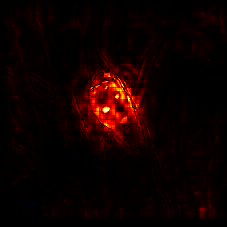
\includegraphics[height=2cm]{data/ladybug_explanation.png}
			};
			\node[] (output) at ($ (n60) + (2, 0) $) {
				"ladybug"
			};

			\newcommand{\outerarrow}{{Latex[length=0.2cm, width=0.3cm]}}
			\draw[\outerarrow-, line width=4pt, draw=gray] (input) to (n00);
			\draw[\outerarrow-, line width=4pt, draw=gray] ($ (n60.east) + (0.076, 0) $) to (output);


		\end{tikzpicture}
	\end{frame}

	% XAI: Flip
	\begin{frame}{Explainable AI}
		\begin{tikzpicture}
			\newcommand{\nodesize}{8pt}
			\newcommand{\hsep}{24pt}
			\newcommand{\vsep}{12pt}

			\newcommand{\arrowwidth}{0.05cm}
			\newcommand{\innerarrow}{{Latex[length=0.1cm, width=0.15cm]}}

			\newcommand{\lrplocation}[1]{($ (0, 0) + ####1 $)}

			\colorlet{lrp-fill}{red}
			\colorlet{predict-fill}{blue}

			\node[circle, inner sep=0pt, fill=none, outer sep=0pt, line width=0pt, draw=none] (n00) at \lrplocation{(-3 * \hsep, 0)} {};
			\node[] at (-5.5, 1.5) {};
			\node[] at (5.1, -1.2) {};

			\draw[black, fill=gray!20] (n00.center) --
						 ($ (n00) + (0, 2*\vsep+0.5*\nodesize+2pt) $) --
						 ($ (n00) + (6*\hsep+0.5*\nodesize+2pt, 2*\vsep+0.5*\nodesize+2pt) $) --
						 ($ (n00) + (6*\hsep+0.5*\nodesize+2pt, -2*\vsep-0.5*\nodesize-2pt) $) --
						 ($ (n00) + (0, -2*\vsep-0.5*\nodesize-2pt) $) --
						 (n00.center);


			\node[circle, inner sep=0pt, fill=none, outer sep=0pt, line width=0pt, draw=none] (n00) at \lrplocation{(-3 * \hsep, 0)} {};

			\node[circle, minimum size=\nodesize, inner sep=0pt, fill={rgb:black,5;orange,1}, outer sep=0pt, line width=0pt, draw={rgb:black,5;orange,1}] (n10) at \lrplocation{(-2 * \hsep, 2 * \vsep)} {};
			\node[circle, minimum size=\nodesize, inner sep=0pt, fill={rgb:black,3;red,1}, outer sep=0pt, line width=0pt, draw={rgb:black,3;red,1}] (n11) at \lrplocation{(-2 * \hsep, 1 * \vsep)} {};
			\node[circle, minimum size=\nodesize, inner sep=0pt, fill=yellow, outer sep=0pt, line width=0pt, draw=yellow] (n12) at \lrplocation{(-2 * \hsep, 0)} {};
			\node[circle, minimum size=\nodesize, inner sep=0pt, fill=black, outer sep=0pt, line width=0pt, draw=black] (n13) at \lrplocation{(-2 * \hsep, -1 * \vsep)} {};
			\node[circle, minimum size=\nodesize, inner sep=0pt, fill=red, outer sep=0pt, line width=0pt, draw=red] (n14) at \lrplocation{(-2 * \hsep, -2 * \vsep)} {};

			\node[circle, minimum size=\nodesize, inner sep=0pt, fill={rgb:black,5;white,2;orange,1}, outer sep=0pt, line width=0pt, draw={rgb:black,5;white,2;orange,1}] (n20) at \lrplocation{(-1 * \hsep, 1.5 * \vsep)} {};
			\node[circle, minimum size=\nodesize, inner sep=0pt, fill={rgb:red,10;yellow,6}, outer sep=0pt, line width=0pt, draw={rgb:red,10;yellow,4}] (n21) at \lrplocation{(-1 * \hsep, 0.5 * \vsep)} {};
			\node[circle, minimum size=\nodesize, inner sep=0pt, fill={rgb:red,10;yellow,1}, outer sep=0pt, line width=0pt, draw={rgb:red,10;yellow,1}] (n22) at \lrplocation{(-1 * \hsep, -0.5 * \vsep)} {};
			\node[circle, minimum size=\nodesize, inner sep=0pt, fill={rgb:black,10;red,2}, outer sep=0pt, line width=0pt, draw={rgb:black,10;red,2}] (n23) at \lrplocation{(-1 * \hsep, -1.5 * \vsep)} {};

			\node[circle, minimum size=\nodesize, inner sep=0pt, fill={rgb:red,3;orange,2}, outer sep=0pt, line width=0pt, draw={rgb:red,3;orange,1}] (n30) at \lrplocation{(0 * \hsep, 1.5 * \vsep)} {};
			\node[circle, minimum size=\nodesize, inner sep=0pt, fill={rgb:yellow,3;orange,1}, outer sep=0pt, line width=0pt, draw={rgb:yellow,3;orange,1}] (n31) at \lrplocation{(0 * \hsep, 0.5 * \vsep)} {};
			\node[circle, minimum size=\nodesize, inner sep=0pt, fill={rgb:black,10;white,5;red,1}, outer sep=0pt, line width=0pt, draw={rgb:black,10;white,5;red,1}] (n32) at \lrplocation{(0 * \hsep, -0.5 * \vsep)} {};
			\node[circle, minimum size=\nodesize, inner sep=0pt, fill={rgb:gray,5;red,1}, outer sep=0pt, line width=0pt, draw={rgb:gray,5;red,1}] (n33) at \lrplocation{(0 * \hsep, -1.5 * \vsep)} {};

			\node[circle, minimum size=\nodesize, inner sep=0pt, fill={rgb:yellow,10;orange,1}, outer sep=0pt, line width=0pt, draw={rgb:yellow,10;orange,1}] (n40) at \lrplocation{(1 * \hsep, 1*\vsep)} {};
			\node[circle, minimum size=\nodesize, inner sep=0pt, fill={rgb:red,1}, outer sep=0pt, line width=0pt, draw={rgb:red,1}] (n41) at \lrplocation{(1 * \hsep, 0*\vsep)} {};
			\node[circle, minimum size=\nodesize, inner sep=0pt, fill={rgb:black,10;white,15;red,2}, outer sep=0pt, line width=0pt, draw={rgb:black,10;white,15;red,2}] (n42) at \lrplocation{(1 * \hsep, -1*\vsep)} {};

			\node[circle, minimum size=\nodesize, inner sep=0pt, fill={rgb:red,5;black,1;yellow,2}, outer sep=0pt, line width=0pt, draw={rgb:red,5;black,1;yellow,2}] (n50) at \lrplocation{(2 * \hsep, 1*\vsep)} {};
			\node[circle, minimum size=\nodesize, inner sep=0pt, fill={rgb:gray,5;red,1}, outer sep=0pt, line width=0pt, draw={rgb:gray,5;red,1}] (n51) at \lrplocation{(2 * \hsep, 0*\vsep)} {};
			\node[circle, minimum size=\nodesize, inner sep=0pt, fill={rgb:yellow,5;orange,1}, outer sep=0pt, line width=0pt, draw={rgb:yellow,5;orange,1}] (n52) at \lrplocation{(2 * \hsep, -1*\vsep)} {};

			\node[circle, minimum size=\nodesize, inner sep=0pt, fill={rgb:orange,7;yellow,4;black,1}, outer sep=0pt, line width=0pt, draw={rgb:orange,7;yellow,4;black,1}] (n60) at \lrplocation{(3 * \hsep, 0)} {};

			\draw[
				color={rgb:black,5;orange,1},
				\innerarrow-,
				line width=\arrowwidth
			] (n00) to [out=20,in=200] (n10) {};
			\draw[
				color={rgb:black,3;red,1},
				\innerarrow-,
				line width=\arrowwidth
			] (n00) to [out=10,in=190] (n11) {};
			\draw[
				color=yellow,
				\innerarrow-,
				line width=\arrowwidth
			] (n00) to [out=0,in=180] (n12) {};
			\draw[
				color=black,
				\innerarrow-,
				line width=\arrowwidth
			] (n00) to [out=-10,in=170] (n13) {};
			\draw[
				color=red,
				\innerarrow-,
				line width=\arrowwidth
			] (n00) to [out=-20,in=160] (n14) {};

			\draw[
				color={rgb:black,5;white,1;orange,1},
				\innerarrow-,
				line width=\arrowwidth
			] (n10) to [out=-5,in=175] (n20) {};
			\draw[
				color={rgb:black,3;orange,1},
				\innerarrow-,
				line width=\arrowwidth
			] (n10) to [out=-15,in=165] (n21) {};
			\draw[
				color={rgb:black,4;red,2;yellow,1},
				\innerarrow-,
				line width=\arrowwidth
			] (n10) to [out=-25,in=155] (n22) {};
			\draw[
				color={rgb:black,3;red,1},
				\innerarrow-,
				line width=\arrowwidth
			] (n10) to [out=-35,in=145] (n23) {};

			\draw[
				color={rgb:black,10;orange,2},
				\innerarrow-,
				line width=\arrowwidth
			] (n11) to [out=5,in=185] (n20) {};
			\draw[
				color={rgb:black,3;orange,1},
				\innerarrow-,
				line width=\arrowwidth
			] (n11) to [out=-5,in=175] (n21) {};
			\draw[
				color={rgb:black,3;red,1},
				\innerarrow-,
				line width=\arrowwidth
			] (n11) to [out=-15,in=165] (n22) {};
			\draw[
				color={rgb:black,10;red,1},
				\innerarrow-,
				line width=\arrowwidth
			] (n11) to [out=-25,in=155] (n23) {};

			\draw[
				color={rgb:black,5;orange,3},
				\innerarrow-,
				line width=\arrowwidth
			] (n12) to [out=15,in=195] (n20) {};
			\draw[
				color={rgb:red,3;yellow,5},
				\innerarrow-,
				line width=\arrowwidth
			] (n12) to [out=5,in=185] (n21) {};
			\draw[
				color={rgb:red,5;yellow,3},
				\innerarrow-,
				line width=\arrowwidth
			] (n12) to [out=-5,in=175] (n22) {};
			\draw[
				color={rgb:black,5;orange,2},
				\innerarrow-,
				line width=\arrowwidth
			] (n12) to [out=-15,in=165] (n23) {};

			\draw[
				color={rgb:black,5;red,1},
				\innerarrow-,
				line width=\arrowwidth
			] (n13) to [out=25,in=205] (n20) {};
			\draw[
				color={rgb:black,5;orange,2},
				\innerarrow-,
				line width=\arrowwidth
			] (n13) to [out=15,in=195] (n21) {};
			\draw[
				color={rgb:black,5;red,3},
				\innerarrow-,
				line width=\arrowwidth
			] (n13) to [out=5,in=185] (n22) {};
			\draw[
				color=black,
				\innerarrow-,
				line width=\arrowwidth
			] (n13) to [out=-5,in=175] (n23) {};

			\draw[
				color={rgb:black,5;orange,2},
				\innerarrow-,
				line width=\arrowwidth
			] (n14) to [out=35,in=215] (n20) {};
			\draw[
				color={rgb:red,3;orange,1},
				\innerarrow-,
				line width=\arrowwidth
			] (n14) to [out=25,in=205] (n21) {};
			\draw[
				color={rgb:red,5;yellow,2},
				\innerarrow-,
				line width=\arrowwidth
			] (n14) to [out=15,in=195] (n22) {};
			\draw[
				color={rgb:black,5;red,3},
				\innerarrow-,
				line width=\arrowwidth
			] (n14) to [out=5,in=185] (n23) {};

			\draw[
				color={rgb:black,1;red,1},
				\innerarrow-,
				line width=\arrowwidth
			] (n20) to [out=0,in=180] (n30) {};
			\draw[
				color={rgb:black,3;orange,1},
				\innerarrow-,
				line width=\arrowwidth
			] (n20) to [out=-10,in=170] (n31) {};
			\draw[
				color={rgb:black,10;red,1},
				\innerarrow-,
				line width=\arrowwidth
			] (n20) to [out=-20,in=160] (n32) {};
			\draw[
				color={rgb:black,5;red,1},
				\innerarrow-,
				line width=\arrowwidth
			] (n20) to [out=-30,in=150] (n33) {};

			\draw[
				color={rgb:orange,5;red,2},
				\innerarrow-,
				line width=\arrowwidth
			] (n21) to [out=10,in=190] (n30) {};
			\draw[
				color={rgb:yellow,10;orange,4},
				\innerarrow-,
				line width=\arrowwidth
			] (n21) to [out=0,in=180] (n31) {};
			\draw[
				color={rgb:black,2;red,1},
				\innerarrow-,
				line width=\arrowwidth
			] (n21) to [out=-10,in=170] (n32) {};
			\draw[
				color={rgb:black,1;orange,2;red,1},
				\innerarrow-,
				line width=\arrowwidth
			] (n21) to [out=-20,in=160] (n33) {};

			\draw[
				color={rgb:red,2;orange,1},
				\innerarrow-,
				line width=\arrowwidth
			] (n22) to [out=20,in=200] (n30) {};
			\draw[
				color={rgb:yellow,2;orange,1},
				\innerarrow-,
				line width=\arrowwidth
			] (n22) to [out=10,in=190] (n31) {};
			\draw[
				color={rgb:black,2;red,2},
				\innerarrow-,
				line width=\arrowwidth
			] (n22) to [out=0,in=180] (n32) {};
			\draw[
				color={rgb:black,2;orange,1},
				\innerarrow-,
				line width=\arrowwidth
			] (n22) to [out=-10,in=170] (n33) {};

			\draw[
				color={rgb:black,4;red,2},
				\innerarrow-,
				line width=\arrowwidth
			] (n23) to [out=30,in=210] (n30) {};
			\draw[
				color={rgb:orange,2;black,1},
				\innerarrow-,
				line width=\arrowwidth
			] (n23) to [out=20,in=200] (n31) {};
			\draw[
				color={rgb:black,5;orange,1},
				\innerarrow-,
				line width=\arrowwidth
			] (n23) to [out=10,in=190] (n32) {};
			\draw[
				color={rgb:black,5;red,2},
				\innerarrow-,
				line width=\arrowwidth
			] (n23) to [out=0,in=180] (n33) {};

			\draw[
				color={rgb:orange,3;red,1},
				\innerarrow-,
				line width=\arrowwidth
			] (n30) to [out=-5,in=175] (n40) {};
			\draw[
				color={rgb:gray,1;orange,1;red,2},
				\innerarrow-,
				line width=\arrowwidth
			] (n30) to [out=-15,in=165] (n41) {};
			\draw[
				color={rgb:orange,2;black,2;white,1},
				\innerarrow-,
				line width=\arrowwidth
			] (n30) to [out=-25,in=155] (n42) {};

			\draw[
				color={rgb:yellow,5;orange,1},
				\innerarrow-,
				line width=\arrowwidth
			] (n31) to [out=5,in=185] (n40) {};
			\draw[
				color={rgb:red,3;orange,1},
				\innerarrow-,
				line width=\arrowwidth
			] (n31) to [out=-5,in=175] (n41) {};
			\draw[
				color={rgb:gray,1;red,2},
				\innerarrow-,
				line width=\arrowwidth
			] (n31) to [out=-15,in=165] (n42) {};

			\draw[
				color={rgb:gray,3;orange,1},
				\innerarrow-,
				line width=\arrowwidth
			] (n32) to [out=15,in=195] (n40) {};
			\draw[
				color={rgb:gray,1;red,1},
				\innerarrow-,
				line width=\arrowwidth
			] (n32) to [out=5,in=185] (n41) {};
			\draw[
				color={rgb:gray,1},
				\innerarrow-,
				line width=\arrowwidth
			] (n32) to [out=-5,in=175] (n42) {};

			\draw[
				color={rgb:gray,2;orange,3},
				\innerarrow-,
				line width=\arrowwidth
			] (n33) to [out=25,in=205] (n40) {};
			\draw[
				color={rgb:gray,1;orange,1},
				\innerarrow-,
				line width=\arrowwidth
			] (n33) to [out=15,in=195] (n41) {};
			\draw[
				color={rgb:gray,3;red,1},
				\innerarrow-,
				line width=\arrowwidth
			] (n33) to [out=5,in=185] (n42) {};

			\draw[
				color={rgb:red,3;yellow,1},
				\innerarrow-,
				line width=\arrowwidth
			] (n40) to [out=0,in=180] (n50) {};
			\draw[
				color={rgb:gray,2;orange,1},
				\innerarrow-,
				line width=\arrowwidth
			] (n40) to [out=-10,in=170] (n51) {};
			\draw[
				color={rgb:yellow,10;orange,1},
				\innerarrow-,
				line width=\arrowwidth
			] (n40) to [out=-20,in=160] (n52) {};

			\draw[
				color={rgb:red,5;black,1;yellow,2},
				\innerarrow-,
				line width=\arrowwidth
			] (n41) to [out=10,in=190] (n50) {};
			\draw[
				color={rgb:gray,7;orange,3},
				\innerarrow-,
				line width=\arrowwidth
			] (n41) to [out=0,in=180] (n51) {};
			\draw[
				color={rgb:yellow,1;orange,2},
				\innerarrow-,
				line width=\arrowwidth
			] (n41) to [out=-10,in=170] (n52) {};

			\draw[
				color={rgb:gray,7;orange,2},
				\innerarrow-,
				line width=\arrowwidth
			] (n42) to [out=20,in=200] (n50) {};
			\draw[
				color={rgb:gray,5;red,1},
				\innerarrow-,
				line width=\arrowwidth
			] (n42) to [out=10,in=190] (n51) {};
			\draw[
				color={rgb:gray,5;red,1;black,2},
				\innerarrow-,
				line width=\arrowwidth
			] (n42) to [out=0,in=180] (n52) {};

			\draw[
				color={rgb:red,5;black,1;yellow,2},
				\innerarrow-,
				line width=\arrowwidth
			] (n50) to [out=-10,in=170] (n60) {};
			\draw[
				color={rgb:gray,5;red,1},
				\innerarrow-,
				line width=\arrowwidth
			] (n51) to [out=0,in=180] (n60) {};
			\draw[
				color={rgb:yellow,5;orange,1},
				\innerarrow-,
				line width=\arrowwidth
			] (n52) to [out=10,in=190] (n60) {};


			\node[] at ($ (n30) + (0, \vsep+0.75*\nodesize) $) {Artificial Neural Network};

			\node[inner sep=0pt, outer sep=0pt, draw=black] (input) at ($ (n00) - (2, 0) $) {
				\scalebox{1}[-1]{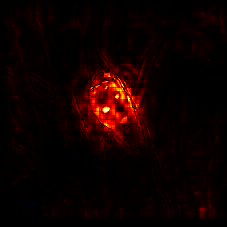
\includegraphics[height=2cm]{data/ladybug_explanation.png}}
			};
			\node[] (output) at ($ (n60) + (2, 0) $) {
				"ladybug"
			};

			\newcommand{\outerarrow}{{Latex[length=0.2cm, width=0.3cm]}}
			\draw[\outerarrow-, line width=4pt, draw=gray] (input) to (n00);
			\draw[\outerarrow-, line width=4pt, draw=gray] ($ (n60.east) + (0.076, 0) $) to (output);


		\end{tikzpicture}
	\end{frame}

	% Dementia: dataset
	\begin{frame}{Dementia: Dataset} % Full dataset
		\pgfplotstableread[col sep=comma]{data/dementia_dataset/dementia_full.csv}\dementiafull
		\pgfplotstableread[col sep=comma]{data/dementia_dataset/dementia_addneuromed_GE_MEDICAL_SYSTEMS.csv}\dementiage
		\pgfplotstableread[col sep=comma]{data/dementia_dataset/dementia_addneuromed_PICKER_International_Inc.csv}\dementiapicker
		\pgfplotstableread[col sep=comma]{data/dementia_dataset/dementia_ADNI_15T.csv}\dementiaadnione
		\pgfplotstableread[col sep=comma]{data/dementia_dataset/dementia_ADNI_30T.csv}\dementiaadnithree
		\pgfplotstableread[col sep=comma]{data/dementia_dataset/dementia_AIBL_10.csv}\dementiaaiblone
		\pgfplotstableread[col sep=comma]{data/dementia_dataset/dementia_AIBL_20.csv}\dementiaaibltwo
		\pgfplotstableread[col sep=comma]{data/dementia_dataset/dementia_miriad_15_T_Signa.csv}\dementiamiriad
		\pgfplotstableread[col sep=comma]{data/dementia_dataset/dementia_oasis3_15T.csv}\dementiaoasisone
		\pgfplotstableread[col sep=comma]{data/dementia_dataset/dementia_oasis3_30T.csv}\dementiaoasisthree
		\pgfplotstableread[col sep=comma]{data/dementia_dataset/dementia_Oslo_GE750.csv}\dementiaoslo
		\pgfplotstableread[col sep=comma]{data/dementia_dataset/dementia_timepoints.csv}\dementiatimepoints

		\def\xmin{46}
		\def\xmax{99}
		\def\ymin{-1.4}
		\def\ymax{1.2}

		\centering
		\vfill
		\begin{tikzpicture}
            \begin{axis}[
                width=\textwidth,
                height=0.45\textwidth,
                xmin=\xmin,
                xmax=\xmax,
                ymin=-1.6,
                ymax=\ymax,
                xtick={55,60,65,70,75,80,85,90,95},
				axis lines=center,
				axis y line=none,
				clip=false
            ]
                \addplot[name path=zero, draw=none] coordinates {(47,0) (97,0)};
                \addplot[name path=fcases, draw=cases-default, very thick] table [x=x, y=F-cases]{\dementiafull};\label{trace:cases}
                \addplot[fill=cases-default, opacity=0.2] fill between [of=zero and fcases];
                \addplot[name path=fcontrols, draw=controls-default, very thick] table [x=x, y=F-controls]{\dementiafull};\label{trace:controls}
                \addplot[fill=controls-default, opacity=0.2] fill between [of=zero and fcontrols];
                \addplot[name path=mcases, draw=cases-default, very thick] table [x=x,y expr=\thisrow{M-cases} * -1]{\dementiafull};
                \addplot[fill=cases-default, opacity=0.2] fill between [of=zero and mcases];
                \addplot[name path=mcontrols, draw=controls-default, very thick] table [x=x,y expr=\thisrow{M-controls} * -1]{\dementiafull};
                \addplot[fill=controls-default, opacity=0.2] fill between [of=zero and mcontrols];
                \node[anchor=south west] at (axis cs: 46, 0.07) {\textbf{FEMALE}};
                \node[anchor=north west] at (axis cs: 46, -0.07) {\textbf{MALE}};
                \node[anchor=south, align=center] (n) at (axis cs: 72.5,-1.6) {n=1708};
                \node[anchor=north,font=\footnotesize] at ($(n.south) + (0,-2.5) $) {\ref{trace:controls} Controls\hspace{0.3cm}\ref{trace:cases} Cases};
            \end{axis}
        \end{tikzpicture}
		\vspace{-0.1cm}

			\newcommand{\scannersubplot}[3]{
				\nextgroupplot[
						axis lines=center,
						axis y line=none,
						xmin=\xmin,
						xmax=\xmax,
						ymin=\ymin - 0.25,
						ymax=\ymax + 0.25,
						xmajorticks=false,
						axis line style={-}
					]

						\addplot[name path=zero, draw=none] coordinates {(\xmin,0) (\xmax,0)};
						\addplot[name path=fcases, draw=cases-default, very thick] table [x=x, y=F-cases]{####1};
						\addplot[fill=cases-default, opacity=0.2] fill between [of=zero and fcases];
						\addplot[name path=fcontrols, draw=controls-default, very thick] table [x=x, y=F-controls]{####1};
						\addplot[fill=controls-default, opacity=0.2] fill between [of=zero and fcontrols];
						\addplot[name path=mcases, draw=cases-default, very thick] table [x=x,y expr=\thisrow{M-cases} * -1]{####1};
						\addplot[fill=cases-default, opacity=0.2] fill between [of=zero and mcases];
						\addplot[name path=mcontrols, draw=controls-default, very thick] table [x=x,y expr=\thisrow{M-controls} * -1]{####1};
						\addplot[fill=controls-default, opacity=0.2] fill between [of=zero and mcontrols];
						\node[anchor=south] at (axis cs: 72.5,1) {\tiny{####2}};
						\node[anchor=north] at (axis cs: 72.5,-1) {\tiny{\textbf{n=####3}}};
			}
				\begin{tikzpicture}
				  \begin{groupplot}[
					  group style={
						  group size=5 by 2,
						  horizontal sep=0.25cm,
						  vertical sep=0.25cm
					  },
					  height=0.314\textwidth,
					  width=0.314\textwidth
				  ]
				 	 \scannersubplot{\dementiaadnithree}{ADNI 3.0T}{506}
					  \scannersubplot{\dementiaoasisthree}{OASIS3 3.0T}{438}
					  \scannersubplot{\dementiaadnione}{ADNI 1.5T}{290}
					  \scannersubplot{\dementiaoslo}{Oslo GE750}{226}
					  \scannersubplot{\dementiaaiblone}{AIBL Site 1}{92}
					  \scannersubplot{\dementiage}{ANM GE}{74}
					  \scannersubplot{\dementiamiriad}{MIRIAD}{38}
					  \scannersubplot{\dementiaaibltwo}{AIBL Site 2}{22}
					  \scannersubplot{\dementiapicker}{ANM Picker}{12}
					  \scannersubplot{\dementiaoasisone}{OASIS3 1.5T}{10}
				  \end{groupplot}
			\end{tikzpicture}

		\vfill
	\end{frame}

	\begin{frame}{Dementia: Predictive performance} % Predictions
		\pgfplotstableread[col sep=comma]{data/test_distributions.csv}\testdistributions
		\pgfplotstableread[col sep=comma]{data/test_predictions.csv}\testpredictions

		\newcommand{\ymin}{-0.35}
		\newcommand{\ymax}{1.05}

		\begin{tikzpicture}
            \begin{axis}[
                name=distributions,
                height=0.4\textwidth,
                width=0.94\textwidth,
                xtick pos=bottom,
                ymajorticks=false,
                xmin=0,
                xmax=1,
                ymin=\ymin,
                ymax=\ymax,
                xlabel=\small{Prediction},
                every tick label/.append style={font=\footnotesize}
            ]
                \addplot[name path=controls, draw=controls-default, very thick] table [x=prediction,y=controls]{\testdistributions};
                \addplot[name path=cases, draw=cases-default, very thick] table [x=prediction,y=cases]{\testdistributions};
                \addplot[name path=zero, draw=black] coordinates {(0,0) (1,0)};
                \addplot[fill=controls-default, opacity=0.2] fill between [of=zero and controls];
                \addplot[fill=cases-default, opacity=0.2] fill between [of=zero and cases];
                \addplot[
                    scatter/classes={
                        control={controls-default, draw=black, opacity=0.5},
                        case={cases-default, draw=black, opacity=0.5}
                    },
                    scatter,
                    mark=*,
                    only marks,
                    point meta=explicit symbolic
                ] table [
                    y expr=\thisrow{y} * -0.15 - 0.1,
                    meta=class,
                ] {\testpredictions};
                \addplot[dashed] coordinates {(0.5, \ymin) (0.5, \ymax)};
            \end{axis}
            % ONLY FOR ALIGNMENT
            \node[anchor=south east] at ($ (distributions.south west) + (0,0.28) $) {\textcolor{white}{\tiny{Controls}}};
            \node[anchor=south east] at ($ (distributions.south west) + (0,0.0) $) {\textcolor{white}{\tiny{Cases}}};

            \node[anchor=south west] at ($ (distributions.south east) + (0,0.28) $) {\tiny{Controls}};
            \node[anchor=south west] at ($ (distributions.south east) + (0,0.0) $) {\tiny{Cases}};
            \node[anchor=south,align=center] at (distributions.north) {\tiny{$t=0.5$}};
        \end{tikzpicture}
	\end{frame}

	\begin{frame}{Dementia: Explanations} % Example relevance maps
		\centering
		\vfill
		\begin{tikzpicture}
			\node[
				minimum height=0.41\textwidth,
				minimum width=0.32\textwidth,
				fill=black
			] (box1) at (0, 0) {};
			\node[anchor=south] at (box1.south) {
				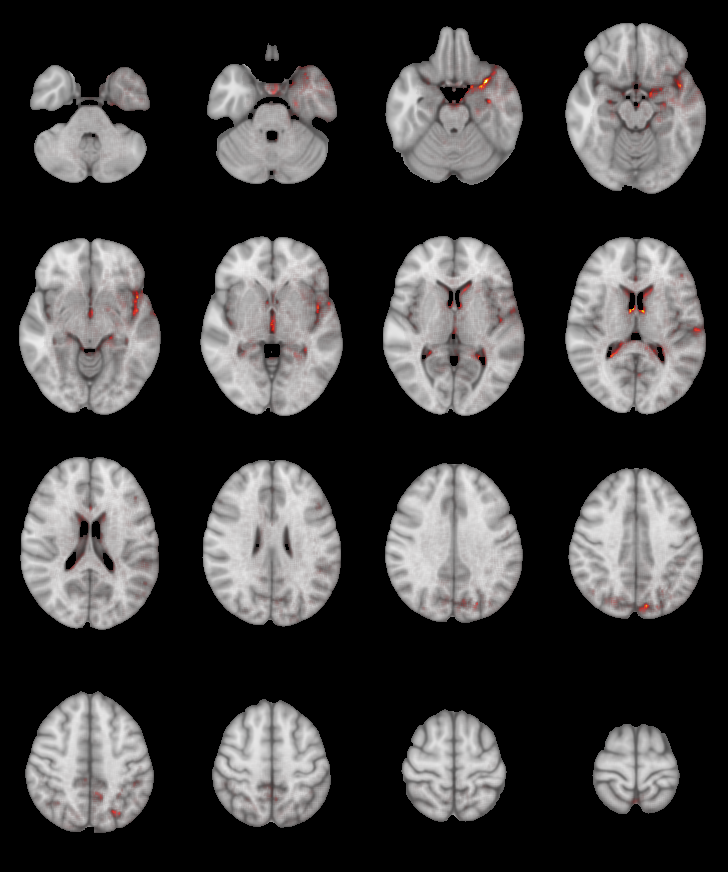
\includegraphics[width=0.31\textwidth]{data/subject1.png}
			};
			\node[anchor=north,inner sep=2pt, text=white, font=\footnotesize] at (box1.north) {Patient 1};

			\node
				[minimum height=0.41\textwidth,
				minimum width=0.32\textwidth,
				fill=black,
				anchor=west
			] (box2) at ($ (box1.east) + (0.05,0) $) {};
			\node[anchor=south] at (box2.south) {
				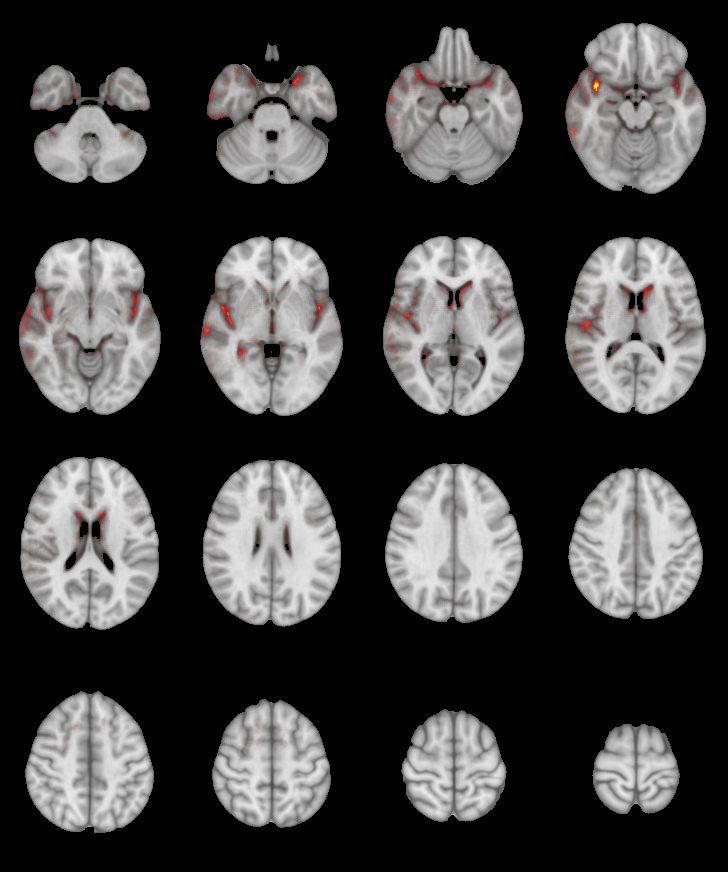
\includegraphics[width=0.31\textwidth]{data/subject2.png}
			};
			\node[anchor=north,inner sep=3pt, text=white, font=\footnotesize] at (box2.north) {Partient 2};

			\node
				[minimum height=0.41\textwidth,
				minimum width=0.32\textwidth,
				fill=black,
				anchor=west
			] (box3) at ($ (box2.east) + (0.05,0) $) {};
			\node[anchor=south] at (box3.south) {
				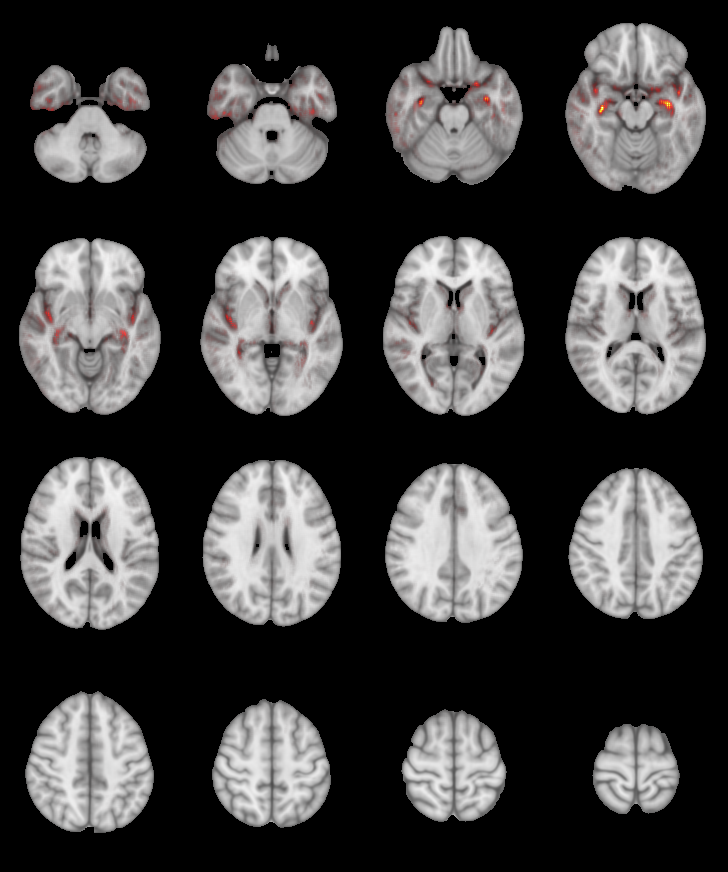
\includegraphics[width=0.31\textwidth]{data/subject3.png}
			};
			\node[anchor=north,inner sep=3pt, text=white, font=\footnotesize] at (box3.north) {Patient 3};

		\end{tikzpicture}
		\vfill
	\end{frame}

	\begin{frame}{Dementia: Validation} % Average maps
		\centering
		\vfill
		\begin{tikzpicture}
			\node[draw=none] at (-2, -2) {};
			\node[draw=none] at (6.5, 2.5) {};
			\node[label={[text depth=0]above:LRP}] at (0, 0) {
				
\includegraphics[width=0.31\textwidth]{data/dementia.png}
			};
		\end{tikzpicture}
		\vfill
	\end{frame}

	\begin{frame}{Dementia: Validation} % Average maps
		\centering
		\vfill
		\begin{tikzpicture}
			\node[draw=none] at (-2, -2) {};
			\node[draw=none] at (6.5, 2.5) {};
			\node[label={[text depth=0]above:LRP}] at (0, 0) {
				
\includegraphics[width=0.31\textwidth]{data/dementia.png}
			};

			\node[label={[text depth=0]above:GingerALE}] at (4.5, 0) {
				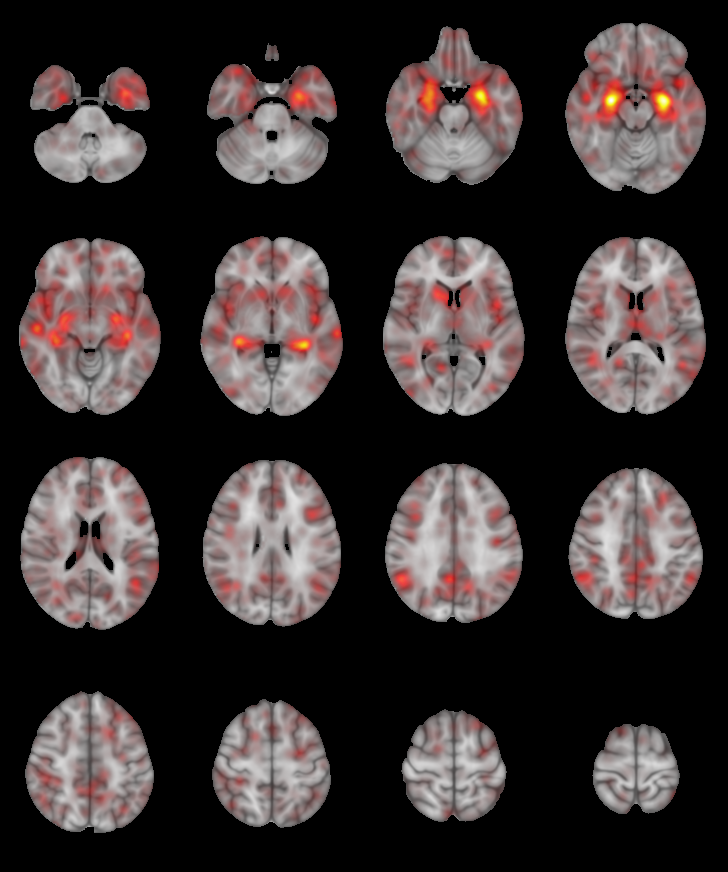
\includegraphics[width=0.31\textwidth]{data/ALE.png}
			};
		\end{tikzpicture}
		\vfill
	\end{frame}

	\begin{frame}{Dementia: Validation} % Overlap
		\centering
		\vfill
		\begin{tikzpicture}
            \node[
                minimum height=0.45\textwidth,
                minimum width=0.33\textwidth,
                fill=black
            ] (box1) at (0, 0) {};
            \node[anchor=south] at ($ (box1.south) + (0, 0.3) $) {
                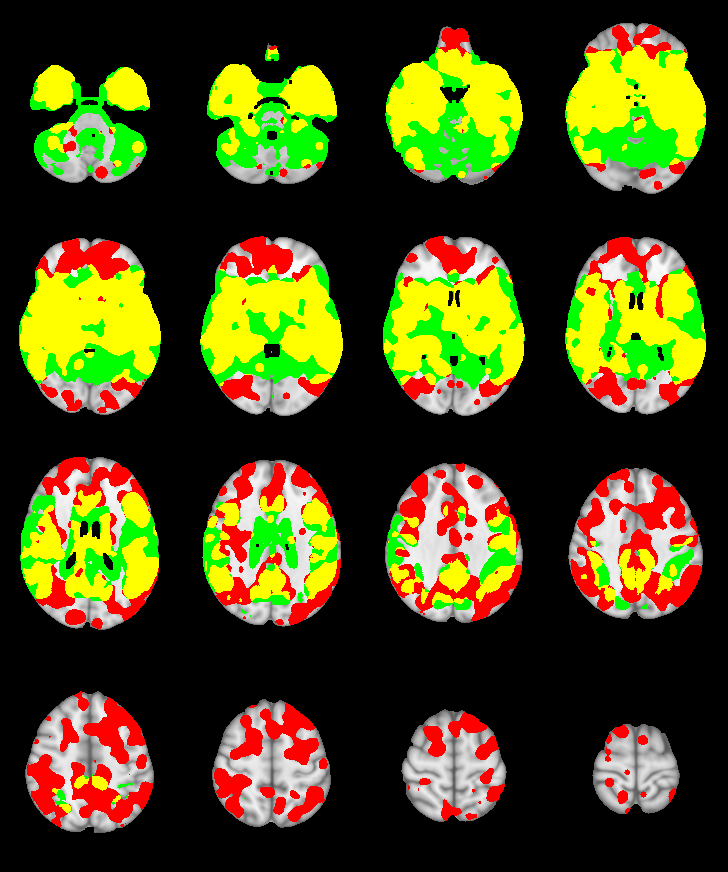
\includegraphics[width=0.31\textwidth]{data/test_50.png}
            };
            \node[anchor=north,inner sep=2pt, text=white, font=\footnotesize] at (box1.north) {50th percentile};

            \node
                [minimum height=0.45\textwidth,
                minimum width=0.33\textwidth,
                fill=black,
                anchor=west
            ] (box2) at ($ (box1.east) + (0.05,0) $) {};
            \node[anchor=south] at ($ (box2.south) + (0, 0.3) $) {
                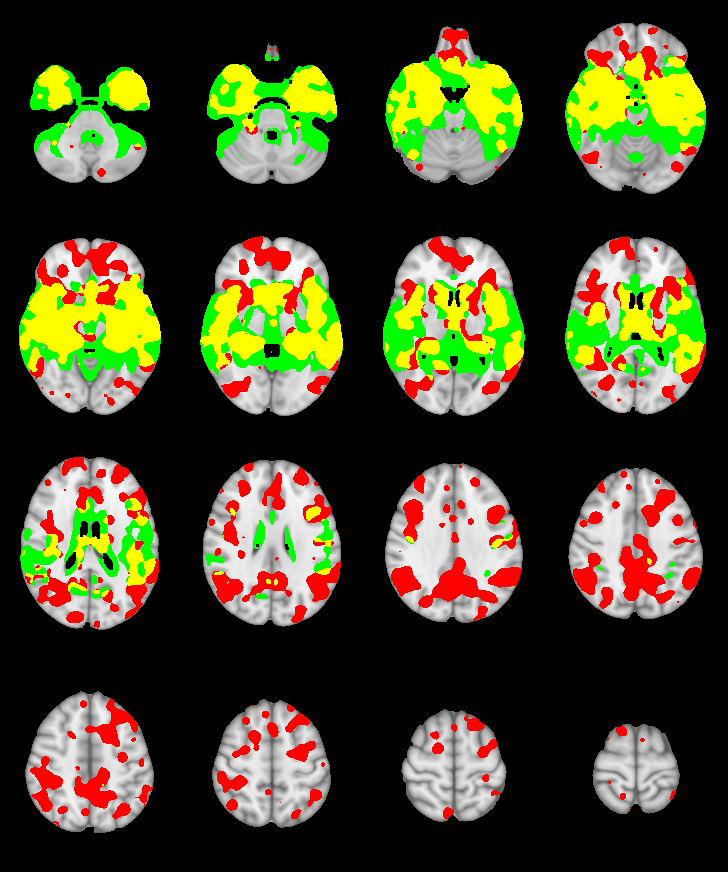
\includegraphics[width=0.31\textwidth]{data/test_70.png}
            };
            \node[anchor=north,inner sep=3pt, text=white, font=\footnotesize] at (box2.north) {70th percentile};

            \node
                [minimum height=0.45\textwidth,
                minimum width=0.33\textwidth,
                fill=black,
                anchor=west
            ] (box3) at ($ (box2.east) + (0.05,0) $) {};
            \node[anchor=south] at ($ (box3.south) + (0, 0.3) $) {
                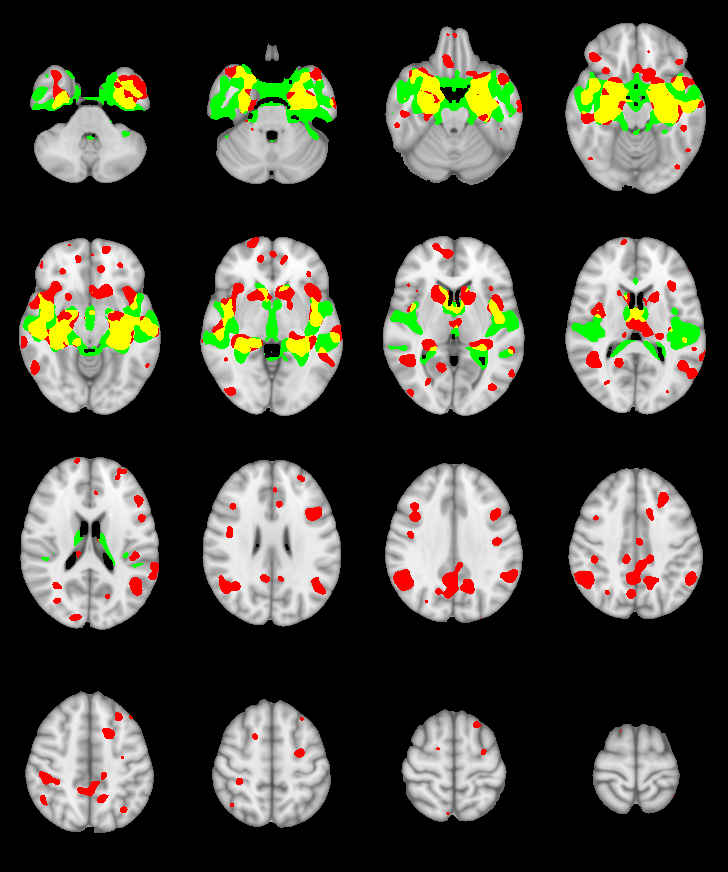
\includegraphics[width=0.31\textwidth]{data/test_90.png}
            };
            \node[anchor=north,inner sep=3pt, text=white, font=\footnotesize] at (box3.north) {90th percentile};

            \node[anchor=south, inner sep=0pt, text depth=0] (overlap) at ($ (box2.south) + (0.1, 0.15) $) {\textcolor{white}{\scriptsize{Overlap}}};
            \node[anchor=east, inner sep=2pt, fill=yellow] (overlap-box) at ($ (overlap.west) + (-0.07, 0) $) {};
            \node[anchor=east, inner sep=0pt,text depth=0] (lrp) at ($ (overlap-box.west) + (-0.2, 0) $) {\textcolor{white}{\scriptsize{LRP}}};
            \node[anchor=east, inner sep=2pt, fill=green] at ($ (lrp.west) + (-0.07, 0) $) {};
            \node[anchor=west, inner sep=2pt, fill=red] (ale-box) at ($ (overlap.east) + (0.2, 0) $) {};
            \node[anchor=west, inner sep=0pt, text depth=0] at ($ (ale-box.east) + (0.07, 0) $) {\textcolor{white}{\scriptsize{ALE}}};

        \end{tikzpicture}
		\vfill
	\end{frame}

	\begin{frame}{Dementia: Validation} % Regions
        \newcommand{\annotation}[4]{
            \node[anchor=####4,align=center,font=\tiny\linespread{0.8}\selectfont,inner sep=2.5pt] at (axis cs: ####2,####3) {####1};
        }
		\vfill
		\centering
		\begin{tikzpicture}
            \begin{axis}[
                width=\textwidth,
                height=0.7\textwidth,
                ylabel=ALE activation,
                xlabel=LRP activation,
                ticks=none,
                xmin=0,
                xmax=1.25,
                ymin=0,
                ymax=1.1,
                axis y line=left,
                axis x line=bottom
            ]
                \addplot[only marks, fill=healthy-default, draw=black] table [col sep=comma, x=lrp, y=ale] {data/regions.csv};

                \annotation{Left Accumbens}{0.90}{1.01}{south}
                \annotation{Right Accumbens}{0.730}{0.865}{south}
                \annotation{Left Amygdala}{1}{0.704}{south}
                \annotation{Right Amygdala}{0.767}{0.651}{north}
                \annotation{Parahippocampal\\Gyrus}{0.591}{0.412}{south}
                \annotation{Heschl's\\Gyrus}{0.782}{0.294}{south}
                \annotation{Lingual\\Gyrus}{0.522}{0.314}{north}
                \annotation{Planum\\Temporale}{0.409}{0.141}{north}
            \end{axis}
        \end{tikzpicture}
		\vfill
	\end{frame}

	\begin{frame}{Mild cognitive impairment: Clinical use case} % Trajectories
		\centering
		\vfill
		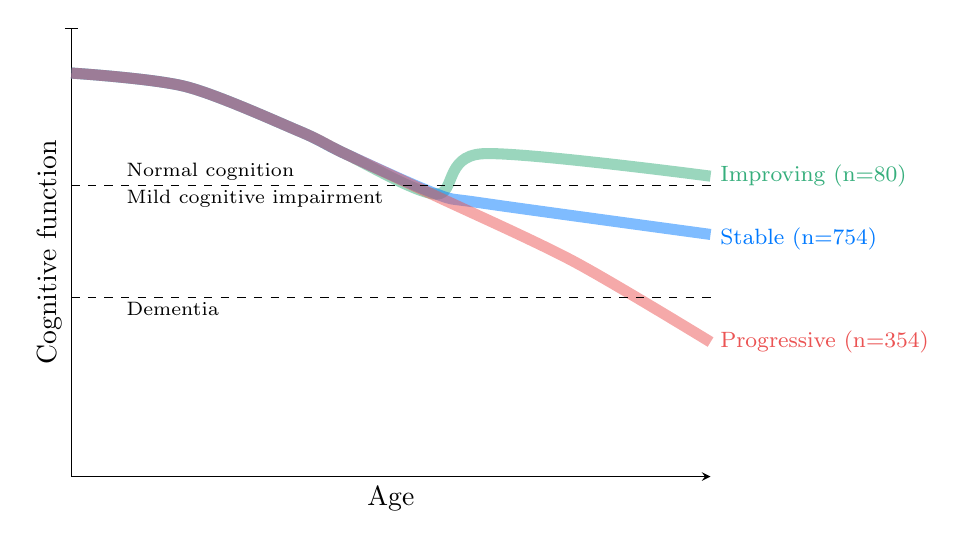
\begin{tikzpicture}
			\begin{axis}[
				height=0.6\textwidth,
				width=0.8\textwidth,
				xlabel={Age},
				ylabel={Cognitive function},
				ticks=none,
				axis x line=bottom,
				axis y line=left,
				y axis line style={-|},
				xmin=0,
				xmax=1.4,
				ymin=0,
				ymax=1,
				clip=false
			]
			\addplot[draw=healthy-default, smooth, line width=4pt, opacity=0.5] coordinates {
				(0, 0.9)
				(0.25, 0.87)
				(0.5, 0.77)
				(0.6, 0.72)
				(0.8, 0.63)
				(0.9, 0.72)
				(1.4, 0.67)
			};
			\addplot[draw=controls-default, smooth, line width=4pt, opacity=0.5] coordinates {
				(0, 0.9)
				(0.25, 0.87)
				(0.5, 0.77)
				(0.6, 0.72)
				(0.8, 0.63)
				(0.9, 0.61)
				(1.4, 0.54)
			};
			\addplot[draw=cases-default, smooth, line width=4pt, opacity=0.5] coordinates {
				(0, 0.9)
				(0.25, 0.87)
				(0.5, 0.77)
				(0.6, 0.72)
				(0.8, 0.625)
				(1.1, 0.48)
				(1.4, 0.3)
			};
			\addplot[dashed] coordinates {
				(0, 0.65)
				(1.4, 0.65)
			};
			\addplot[dashed] coordinates {
				(0, 0.4)
				(1.4, 0.4)
			};
			\node[anchor=south west] at (axis cs: 0.1, 0.64) {\scriptsize{Normal cognition}};
			\node[anchor=north west] at (axis cs: 0.1, 0.66) {\scriptsize{Mild cognitive impairment}};
			\node[anchor=north west] at (axis cs: 0.1, 0.41) {\scriptsize{Dementia}};
			\node[anchor=west] at (axis cs: 1.4, 0.67) {\textcolor{healthy-default}{\footnotesize{Improving (n=80)}}};
			\node[anchor=west] at (axis cs: 1.4, 0.53) {\textcolor{controls-default}{\footnotesize{Stable (n=754)}}};
			\node[anchor=west] at (axis cs: 1.4, 0.3) {\textcolor{cases-default}{\footnotesize{Progressive (n=354)}}};
			\end{axis}
		\end{tikzpicture}
		\vfill
	\end{frame}

	\begin{frame}{Mild cognitive impairment: Prediction} % Predictions
		\begin{tikzpicture}
			\begin{axis}[
				height=0.6\textwidth,
				width=1.1\textwidth,
				xmin=0,
				xmax=1,
				ymin=0,
				ymax=1.05,
				ymajorticks=false,
				xtick pos=bottom,
				xlabel=Prediction,
			]
				\addplot[draw=none, name path=zero] coordinates {(0, 0) (1, 0)};
				\addplot[
					draw=healthy-default,
					very thick,
					name path=improved
				] table [
					col sep=comma,
					x=points,
					y=improved,
				] {data/distributions.csv};

				\addplot[healthy-default, opacity=0.2] fill between [
					of=zero and improved
				];

				\addplot[
					draw=controls-default,
					very thick,
					name path=stable
				] table [
					col sep=comma,
					x=points,
					y=stable
				] {data/distributions.csv};

				\addplot[controls-default, opacity=0.2] fill between [
					of=zero and stable
				];

				\addplot[
					draw=cases-default,
					very thick,
					name path=declined
				] table [
					col sep=comma,
					x=points,
					y=declined
				] {data/distributions.csv};

				\addplot[cases-default, opacity=0.2] fill between [
					of=zero and declined
				];

				\addplot[
					only marks,
					fill=healthy-default,
					mark options={mark size=3pt},
					draw=healthy-default
				] coordinates {(0.105, 4.418/7.838)};

				\addplot[
					only marks,
					fill=controls-default,
					mark options={mark size=3pt},
					draw=controls-default
				] coordinates {(0.333, 0.592/7.838)};

				\addplot[
					only marks,
					fill=cases-default,
					mark options={mark size=3pt},
					draw=cases-default
				] coordinates {(0.649, 0.829/7.838)};

				\node[anchor=south] at (axis cs: 0.649, 0.95/7.838) {\scriptsize{\textcolor{cases-default}{0.649}}};
				\node[anchor=south] at (axis cs: 0.333, 0.72/7.838) {\scriptsize{\textcolor{controls-default}{0.333}}};
				\node[anchor=west] at (axis cs: 0.11, 4.418/7.838) {\scriptsize{\textcolor{healthy-default}{0.105}}};

				\node[circle, inner sep=2pt, label={[text depth=0]right:Improving}, fill=healthy-default!20, draw=healthy-default] (imci) at (axis cs: 0.81, 0.98) {};
				\node[circle, inner sep=2pt, anchor=north, label={[text depth=0]right:Stable}, fill=controls-default!20, draw=controls-default] (smci) at ($ (imci.south) + (0, -2) $) {};
				\node[circle, inner sep=2pt, anchor=north, label={[text depth=0]right:Progressive}, fill=cases-default!20, draw=cases-default] (pmci) at ($ (smci.south) + (0, -2) $) {};
			\end{axis}
	\end{tikzpicture}
	\end{frame}

	\begin{frame}{Mild cognitive impairment: Relevance maps} % PCA components
		\centering
		\vfill
		\newcommand{\mriwidth}{2.2cm}
        \newcommand{\gap}{0.00cm}
        \begin{tikzpicture}
			\node[] at (-1.4, 2.1) {};
			\node[] at (8.8, -3.6) {};

            \node[label={[text depth=0pt]above:Component 0}] (first) at (0, 0) {
                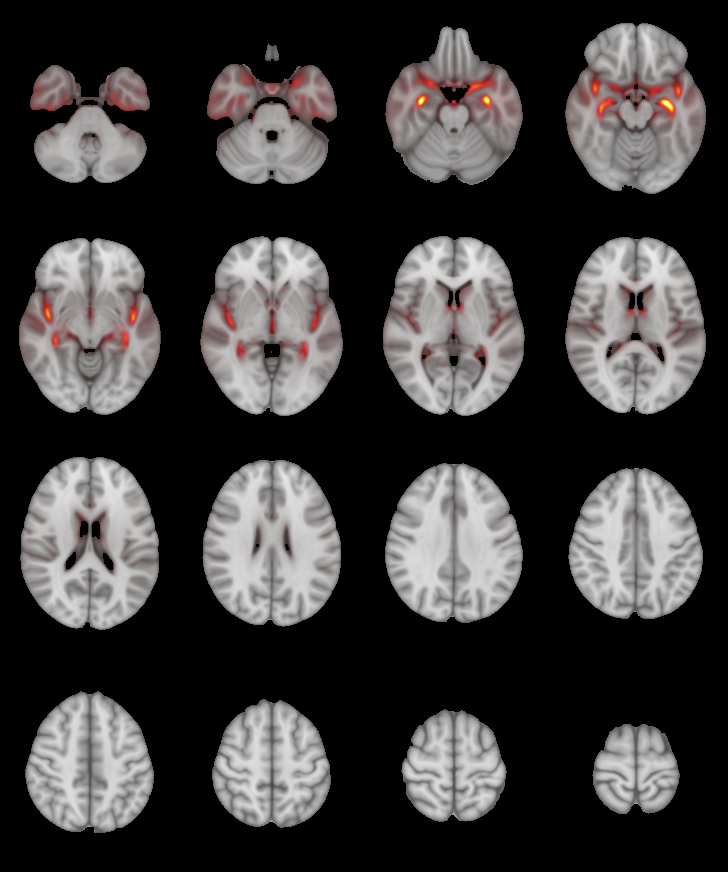
\includegraphics[
                    width=\mriwidth,
                    clip=true,
                    trim = 192mm 232mm 0mm 0mm
                ]{data/components/component_0.png}
            };
            \node[anchor=west, label={[text depth=0pt]above:Component 1}] (second) at ($ (first.east) + (\gap, 0) $) {
                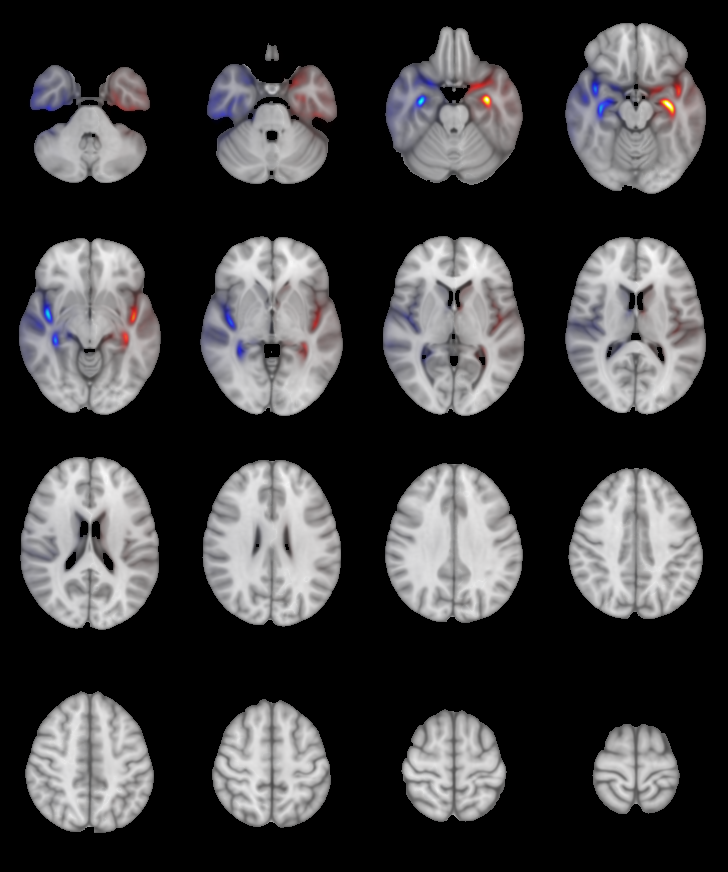
\includegraphics[
                    width=\mriwidth,
                    clip=true,
                    trim = 192mm 232mm 0mm 0mm
                ]{data/components/component_1.png}
            };

            \node[anchor=west, label={[text depth=0pt]above:Component 2}] (third) at ($ (second.east) + (\gap, 0) $) {
                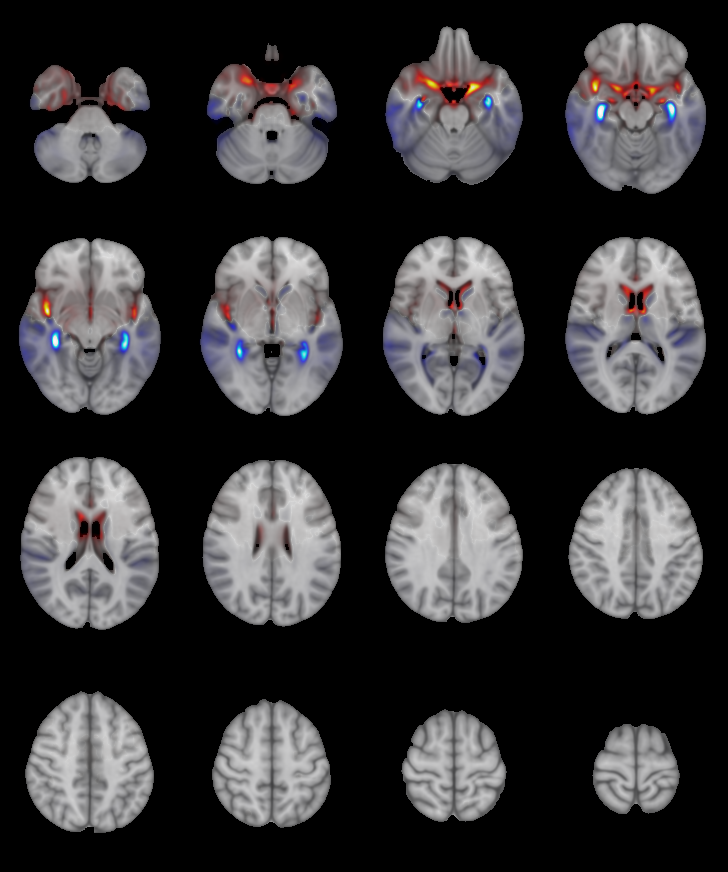
\includegraphics[
                    width=\mriwidth,
                    clip=true,
                    trim = 192mm 232mm 0mm 0mm
                ]{data/components/component_2.png}
            };

            \node[anchor=west, label={[text depth=0pt]above:Component 3}] (fourth) at ($ (third.east) + (\gap, 0) $) {
                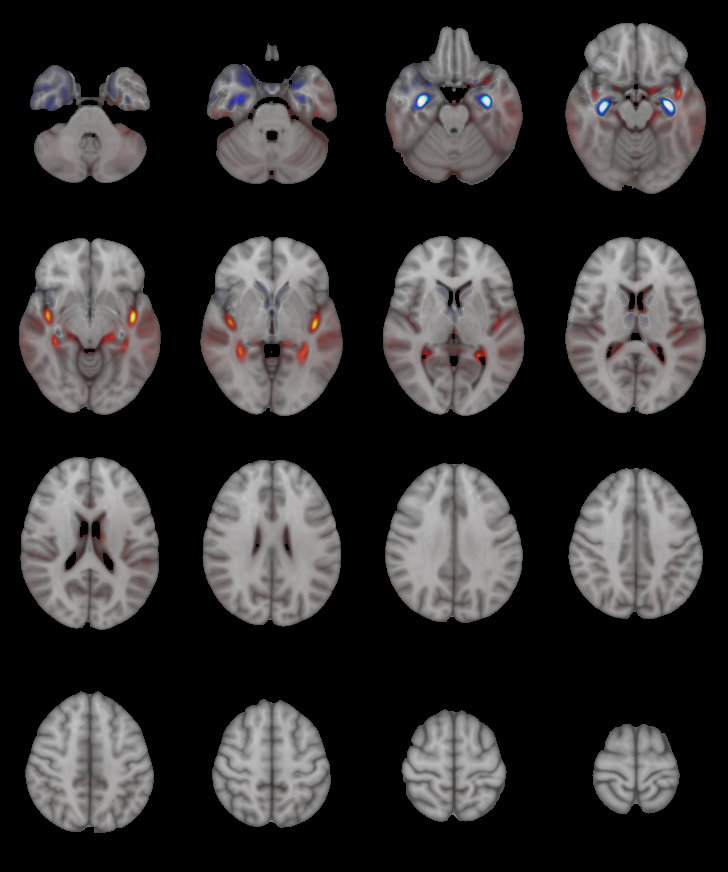
\includegraphics[
                    width=\mriwidth,
                    clip=true,
                    trim = 192mm 232mm 0mm 0mm
                ]{data/components/component_3.png}
            };
        \end{tikzpicture}
		\vfill
	\end{frame}

	\begin{frame}{Mild cognitive impairment: Survival analyses} % Survival
		\centering
		\vfill
		\newcommand{\mriwidth}{2.2cm}
        \newcommand{\gap}{0.00cm}

        \colorlet{ninety}{cases-default}
        \colorlet{fifty}{controls-default}
        \colorlet{ten}{healthy-default}

        \newsavebox{\first}
        \sbox{\first}{%
            \begin{tikzpicture}
                \begin{axis}[
                    height=3cm,
                    width=1.71 * \mriwidth,
                    ylabel style={
                        align=center,
                        font=\scriptsize\linespread{0.8}\selectfont,
                        at={(axis description cs:1.2,0.5)}
                    },
                    xlabel style={
                        at={(axis description cs: 0.5, -0.2)}
                    },
                    ylabel={Healthy\\fraction},
                    xlabel=\scriptsize{Age},
                    every tick label/.append style={font=\tiny},
                    xtick pos=bottom,
                    ytick pos=right,
                    ymin=0,
                    ymax=1,
                    xmin=62,
                    xmax=95,
                    ytick={0, 0.2, 0.4, 0.6, 0.8, 1.0},
                    ytick style={draw=none},
                    ymajorgrids=true,
                    grid style={line width=.5pt, draw=gray!25},
                ]

                \addplot[fifty, very thick] table [col sep=comma, x=age, y=baseline] {data/survival/survival_0.csv};
                \addplot[ten, very thick] table [col sep=comma, x=age, y=fifth] {data/survival/survival_0.csv};
                \addplot[ninety, very thick] table [col sep=comma, x=age, y=ninetyfifth] {data/survival/survival_0.csv};
                \node[anchor=south west,font=\scriptsize] at (axis cs: 62, 0.3) {
                    $\beta\mathrm{=}0.68$
                };
                \node[anchor=south west,font=\scriptsize] at (axis cs: 62, 0.1) {
                    $p\mathrm{=}1.59\times10^{-66}$
                };
                \end{axis}
            \end{tikzpicture}
            }

        \newsavebox{\second}
        \sbox{\second}{%
            \begin{tikzpicture}
                \begin{axis}[
                    height=3cm,
                    width=1.71 * \mriwidth,
                    every tick label/.append style={font=\tiny},
                    xtick pos=bottom,
                    ytick pos=right,
                    ymin=0,
                    ymax=1,
                    xmin=62,
                    xmax=95,
                    ytick={0, 0.2, 0.4, 0.6, 0.8, 1.0},
                    yticklabels={,,},
                    ytick style={draw=none},
                    ymajorgrids=true,
                    grid style={line width=.5pt, draw=gray!25},
                ]

                \addplot[fifty, very thick] table [col sep=comma, x=age, y=baseline] {data/survival/survival_2.csv};
                \addplot[ten, very thick] table [col sep=comma, x=age, y=fifth] {data/survival/survival_2.csv};
                \addplot[ninety, very thick] table [col sep=comma, x=age, y=ninetyfifth] {data/survival/survival_2.csv};
                \node[anchor=south west,font=\scriptsize] at (axis cs: 62, 0.3) {
                    $\beta\mathrm{=}-0.24$
                };
                \node[anchor=south west,font=\scriptsize] at (axis cs: 62, 0.1) {
                    $p\mathrm{=}4.40\times10^{-26}$
                };
                \end{axis}
            \end{tikzpicture}
        }

        \newsavebox{\third}
        \sbox{\third}{%
            \begin{tikzpicture}
                \begin{axis}[
                    height=3cm,
                    width=1.71 * \mriwidth,
                    every tick label/.append style={font=\tiny},
                    xtick pos=bottom,
                    ytick pos=right,
                    ymin=0,
                    ymax=1,
                    xmin=62,
                    xmax=95,
                    ytick={0, 0.2, 0.4, 0.6, 0.8, 1.0},
                    yticklabels={,,},
                    ytick style={draw=none},
                    ymajorgrids=true,
                    grid style={line width=.5pt, draw=gray!25},
                ]

                \addplot[fifty, very thick] table [col sep=comma, x=age, y=baseline] {data/survival/survival_3.csv};
                \addplot[ten, very thick] table [col sep=comma, x=age, y=fifth] {data/survival/survival_3.csv};
                \addplot[ninety, very thick] table [col sep=comma, x=age, y=ninetyfifth] {data/survival/survival_3.csv};
                \node[anchor=south west,font=\scriptsize] at (axis cs: 62, 0.3) {
                    $\beta\mathrm{=}0.22$
                };
                \node[anchor=south west,font=\scriptsize] at (axis cs: 62, 0.1) {
                    $p\mathrm{=}2.31\times10^{-20}$
                };
                \end{axis}
            \end{tikzpicture}
        }

        \begin{tikzpicture}
			\node[] at (-1.4, 2.1) {};
			\node[] at (8.8, -3.6) {};

            \node[label={[text depth=0pt]above:Component 0}] (first) at (0, 0) {
                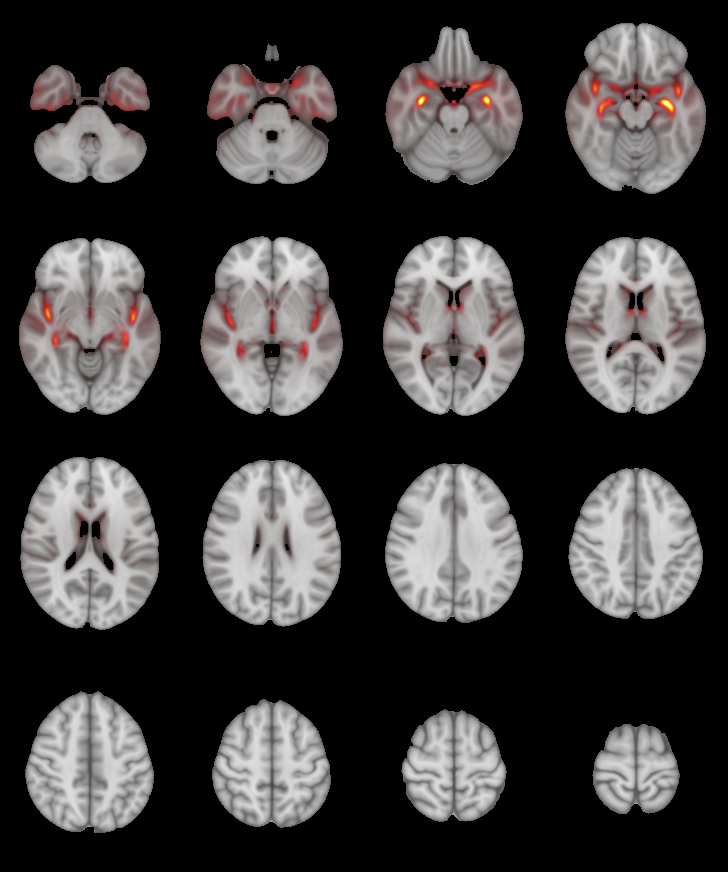
\includegraphics[
                    width=\mriwidth,
                    clip=true,
                    trim = 192mm 232mm 0mm 0mm
                ]{data/components/component_0.png}
            };
            \node[anchor=north west] (first-survival) at ($ (first.south west) + (0, 0.35) $) {
                \usebox{\first}
            };

            \node[anchor=west, label={[text depth=0pt]above:Component 1}] (second) at ($ (first.east) + (\gap, 0) $) {
                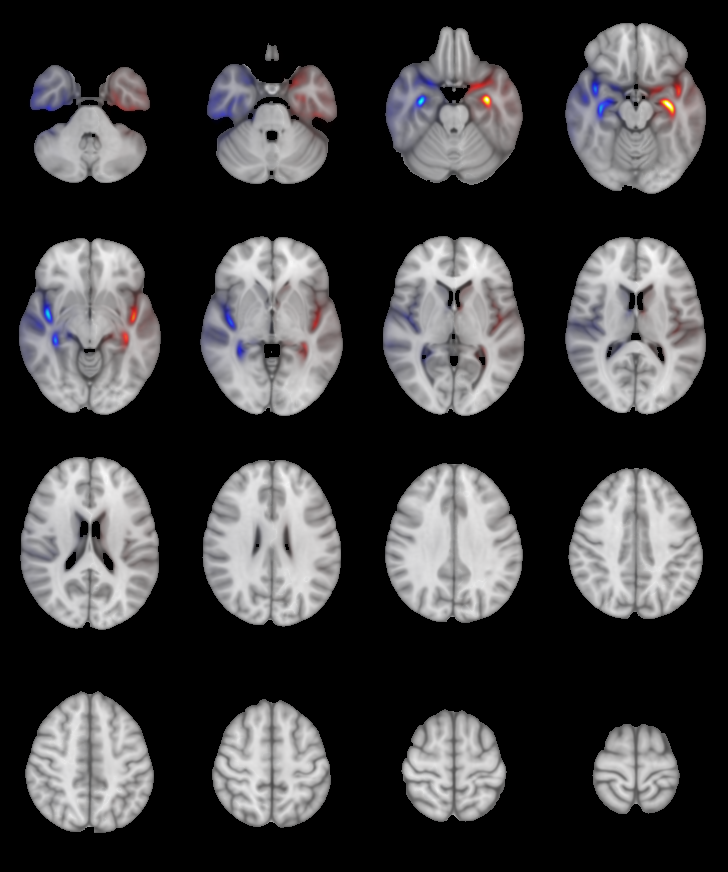
\includegraphics[
                    width=\mriwidth,
                    clip=true,
                    trim = 192mm 232mm 0mm 0mm
                ]{data/components/component_1.png}
            };

            \node[anchor=west, label={[text depth=0pt]above:Component 2}] (third) at ($ (second.east) + (\gap, 0) $) {
                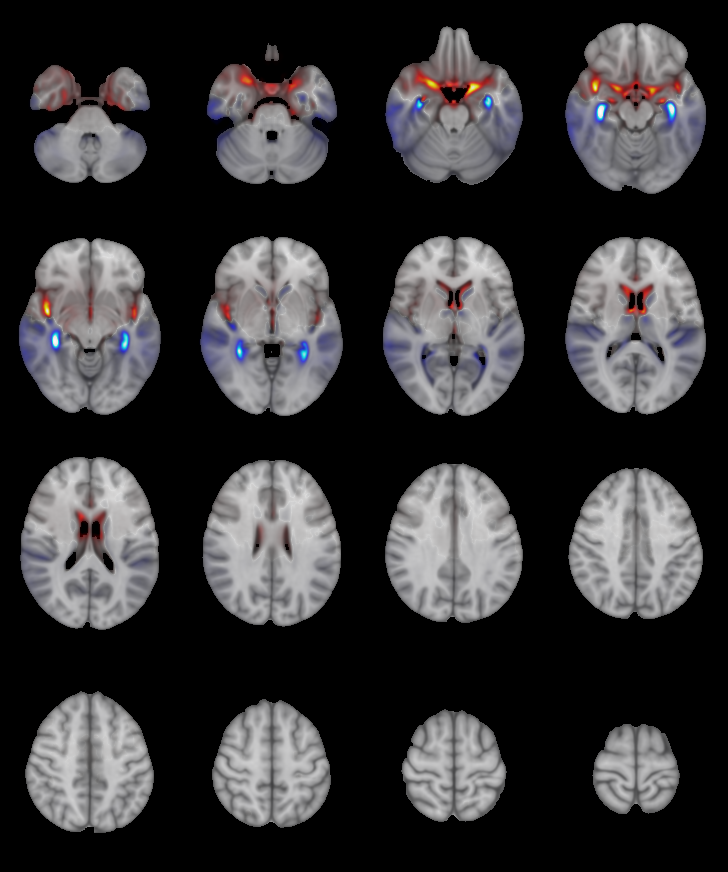
\includegraphics[
                    width=\mriwidth,
                    clip=true,
                    trim = 192mm 232mm 0mm 0mm
                ]{data/components/component_2.png}
            };
            \node[anchor=north west] (third-survival) at ($ (third.south west) + (0, 0.3) $) {
                \usebox{\second}
            };

            \node[anchor=west, label={[text depth=0pt]above:Component 3}] (fourth) at ($ (third.east) + (\gap, 0) $) {
                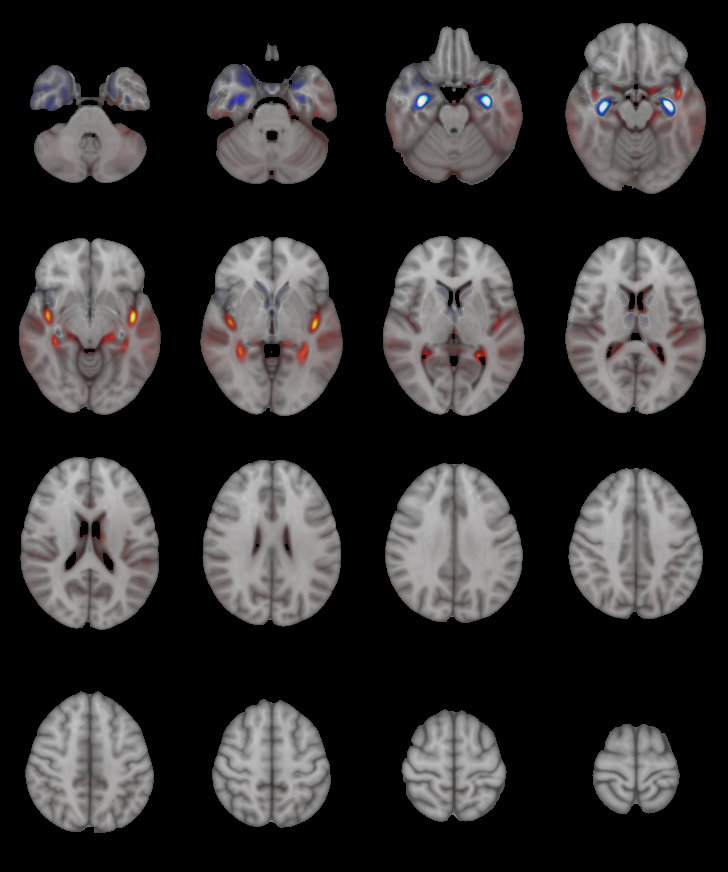
\includegraphics[
                    width=\mriwidth,
                    clip=true,
                    trim = 192mm 232mm 0mm 0mm
                ]{data/components/component_3.png}
            };
            \node[anchor=north west] (fourth-survival) at ($ (fourth.south west) + (0, 0.3) $) {
                \usebox{\third}
            };

            \node[anchor=north east, inner sep=2pt] (legend-header) at ($ (third-survival.north west) - (0.22, 0.33) $) {\scriptsize{\underline{Percentiles}}};
            \node[anchor=north west, inner sep=1pt] (tenth) at ($ (legend-header.south east) - (0.83, 0) $) {\scriptsize{5th}};
            \node[anchor=north west, inner sep=1pt] (fiftieth) at (tenth.south west) {\scriptsize{50th}};
            \node[anchor=north west, inner sep=1pt] (ninetyeth) at (fiftieth.south west) {\scriptsize{95th}};
            \draw[draw=ten, very thick, text depth=0] ($ (tenth.west) + (-0.43, 0) $) -- ($ (tenth.west) + (-0.05, 0) $);
            \draw[draw=fifty, very thick, text depth=0] ($ (fiftieth.west) + (-0.43, 0) $) -- ($ (fiftieth.west) + (-0.05, 0) $);
            \draw[draw=ninety, very thick, text depth=0] ($ (ninetyeth.west) + (-0.43, 0) $) -- ($ (ninetyeth.west) + (-0.05, 0) $);
        \end{tikzpicture}
		\vfill
	\end{frame}

	\begin{frame}{Mild cognitive impairment: Prognosis} % Prognosis
		\centering
		\vfill
		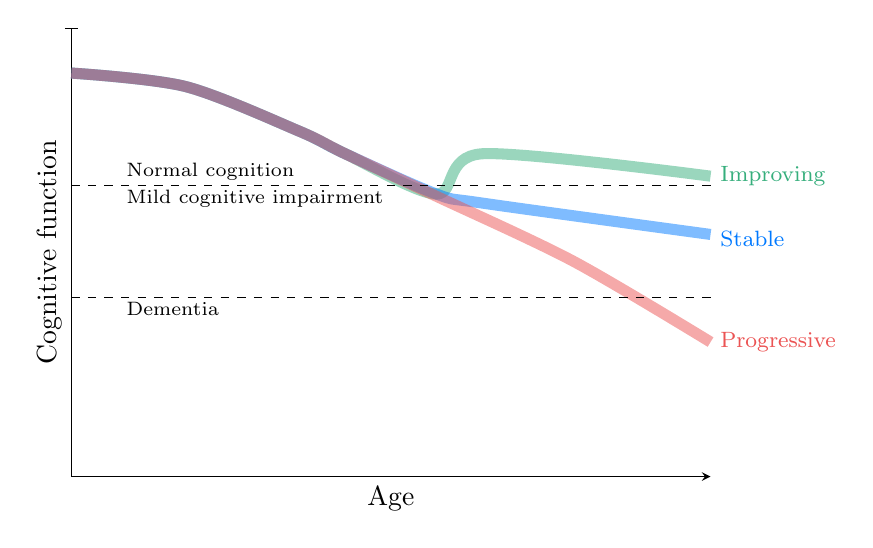
\begin{tikzpicture}
			\begin{axis}[
				height=0.6\textwidth,
				width=0.8\textwidth,
				xlabel={Age},
				ylabel={Cognitive function},
				ticks=none,
				axis x line=bottom,
				axis y line=left,
				y axis line style={-|},
				xmin=0,
				xmax=1.4,
				ymin=0,
				ymax=1,
				clip=false
			]
			\addplot[draw=healthy-default, smooth, line width=4pt, opacity=0.5] coordinates {
				(0, 0.9)
				(0.25, 0.87)
				(0.5, 0.77)
				(0.6, 0.72)
				(0.8, 0.63)
				(0.9, 0.72)
				(1.4, 0.67)
			};
			\addplot[draw=controls-default, smooth, line width=4pt, opacity=0.5] coordinates {
				(0, 0.9)
				(0.25, 0.87)
				(0.5, 0.77)
				(0.6, 0.72)
				(0.8, 0.63)
				(0.9, 0.61)
				(1.4, 0.54)
			};
			\addplot[draw=cases-default, smooth, line width=4pt, opacity=0.5] coordinates {
				(0, 0.9)
				(0.25, 0.87)
				(0.5, 0.77)
				(0.6, 0.72)
				(0.8, 0.625)
				(1.1, 0.48)
				(1.4, 0.3)
			};
			\addplot[dashed] coordinates {
				(0, 0.65)
				(1.4, 0.65)
			};
			\addplot[dashed] coordinates {
				(0, 0.4)
				(1.4, 0.4)
			};
			\node[anchor=south west] at (axis cs: 0.1, 0.64) {\scriptsize{Normal cognition}};
			\node[anchor=north west] at (axis cs: 0.1, 0.66) {\scriptsize{Mild cognitive impairment}};
			\node[anchor=north west] at (axis cs: 0.1, 0.41) {\scriptsize{Dementia}};
			\node[anchor=west] at (axis cs: 1.4, 0.67) {\textcolor{healthy-default}{\footnotesize{Improving}}};
			\node[anchor=west] at (axis cs: 1.4, 0.53) {\textcolor{controls-default}{\footnotesize{Stable}}};
			\node[anchor=west] at (axis cs: 1.4, 0.3) {\textcolor{cases-default}{\footnotesize{Progressive}}};
			\end{axis}
		\end{tikzpicture}
		\vfill
	\end{frame}

	\begin{frame}{Mild cognitive impairment: Prognosis} % Prognosis
		\centering
		\vfill
		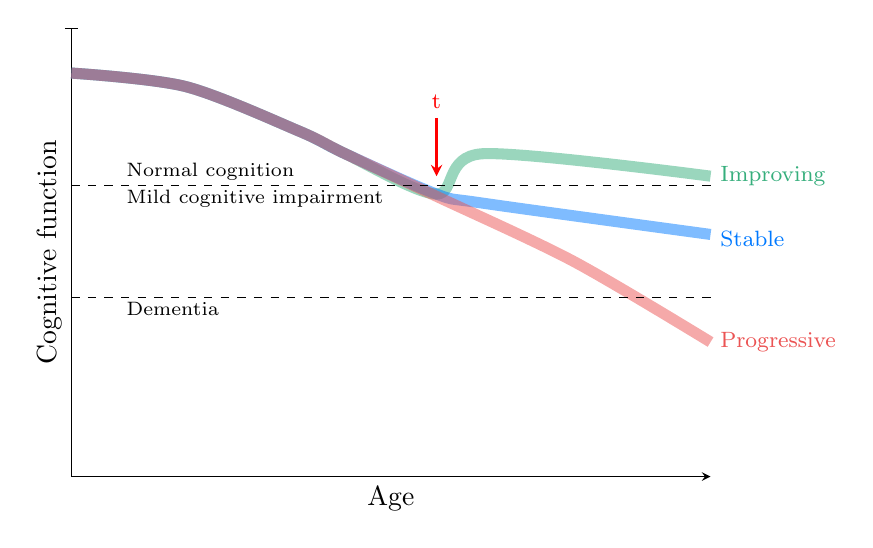
\begin{tikzpicture}
			\begin{axis}[
				height=0.6\textwidth,
				width=0.8\textwidth,
				xlabel={Age},
				ylabel={Cognitive function},
				ticks=none,
				axis x line=bottom,
				axis y line=left,
				y axis line style={-|},
				xmin=0,
				xmax=1.4,
				ymin=0,
				ymax=1,
				clip=false
			]
			\addplot[draw=healthy-default, smooth, line width=4pt, opacity=0.5] coordinates {
				(0, 0.9)
				(0.25, 0.87)
				(0.5, 0.77)
				(0.6, 0.72)
				(0.8, 0.63)
				(0.9, 0.72)
				(1.4, 0.67)
			};
			\addplot[draw=controls-default, smooth, line width=4pt, opacity=0.5] coordinates {
				(0, 0.9)
				(0.25, 0.87)
				(0.5, 0.77)
				(0.6, 0.72)
				(0.8, 0.63)
				(0.9, 0.61)
				(1.4, 0.54)
			};
			\addplot[draw=cases-default, smooth, line width=4pt, opacity=0.5] coordinates {
				(0, 0.9)
				(0.25, 0.87)
				(0.5, 0.77)
				(0.6, 0.72)
				(0.8, 0.625)
				(1.1, 0.48)
				(1.4, 0.3)
			};
			\addplot[dashed] coordinates {
				(0, 0.65)
				(1.4, 0.65)
			};
			\addplot[dashed] coordinates {
				(0, 0.4)
				(1.4, 0.4)
			};
			\node[anchor=south west] at (axis cs: 0.1, 0.64) {\scriptsize{Normal cognition}};
			\node[anchor=north west] at (axis cs: 0.1, 0.66) {\scriptsize{Mild cognitive impairment}};
			\node[anchor=north west] at (axis cs: 0.1, 0.41) {\scriptsize{Dementia}};
			\node[anchor=west] at (axis cs: 1.4, 0.67) {\textcolor{healthy-default}{\footnotesize{Improving}}};
			\node[anchor=west] at (axis cs: 1.4, 0.53) {\textcolor{controls-default}{\footnotesize{Stable}}};
			\node[anchor=west] at (axis cs: 1.4, 0.3) {\textcolor{cases-default}{\footnotesize{Progressive}}};
			\draw[-stealth, red, thick] (axis cs: 0.8, 0.8) -- (axis cs: 0.8, 0.67);
			\node[anchor=south] at (axis cs: 0.8, 0.8) {\textcolor{red}{\footnotesize{t}}};
			\end{axis}
		\end{tikzpicture}
		\vfill
	\end{frame}

	\begin{frame}{Mild cognitive impairment: Prognosis} % Prognosis
		\centering
		\vfill
		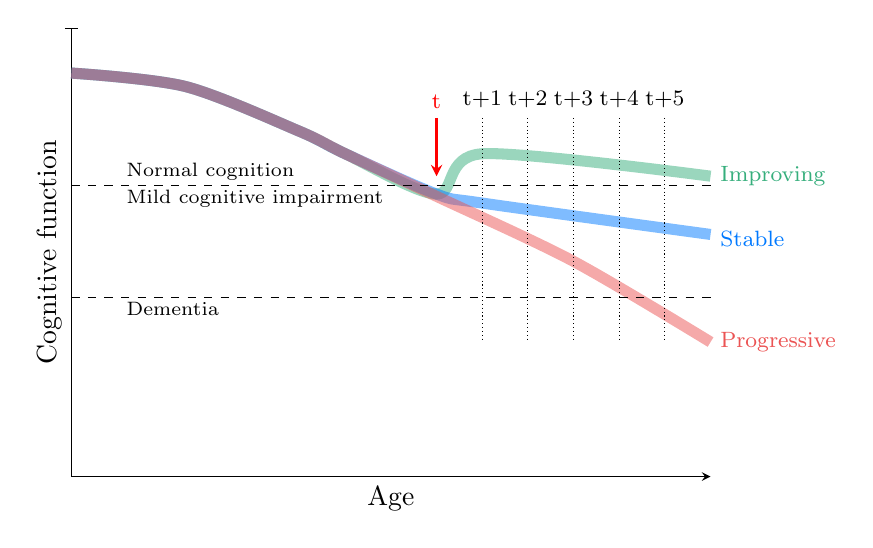
\begin{tikzpicture}
			\begin{axis}[
				height=0.6\textwidth,
				width=0.8\textwidth,
				xlabel={Age},
				ylabel={Cognitive function},
				ticks=none,
				axis x line=bottom,
				axis y line=left,
				y axis line style={-|},
				xmin=0,
				xmax=1.4,
				ymin=0,
				ymax=1,
				clip=false
			]
			\addplot[draw=healthy-default, smooth, line width=4pt, opacity=0.5] coordinates {
				(0, 0.9)
				(0.25, 0.87)
				(0.5, 0.77)
				(0.6, 0.72)
				(0.8, 0.63)
				(0.9, 0.72)
				(1.4, 0.67)
			};
			\addplot[draw=controls-default, smooth, line width=4pt, opacity=0.5] coordinates {
				(0, 0.9)
				(0.25, 0.87)
				(0.5, 0.77)
				(0.6, 0.72)
				(0.8, 0.63)
				(0.9, 0.61)
				(1.4, 0.54)
			};
			\addplot[draw=cases-default, smooth, line width=4pt, opacity=0.5] coordinates {
				(0, 0.9)
				(0.25, 0.87)
				(0.5, 0.77)
				(0.6, 0.72)
				(0.8, 0.625)
				(1.1, 0.48)
				(1.4, 0.3)
			};
			\addplot[dashed] coordinates {
				(0, 0.65)
				(1.4, 0.65)
			};
			\addplot[dashed] coordinates {
				(0, 0.4)
				(1.4, 0.4)
			};
			\node[anchor=south west] at (axis cs: 0.1, 0.64) {\scriptsize{Normal cognition}};
			\node[anchor=north west] at (axis cs: 0.1, 0.66) {\scriptsize{Mild cognitive impairment}};
			\node[anchor=north west] at (axis cs: 0.1, 0.41) {\scriptsize{Dementia}};
			\node[anchor=west] at (axis cs: 1.4, 0.67) {\textcolor{healthy-default}{\footnotesize{Improving}}};
			\node[anchor=west] at (axis cs: 1.4, 0.53) {\textcolor{controls-default}{\footnotesize{Stable}}};
			\node[anchor=west] at (axis cs: 1.4, 0.3) {\textcolor{cases-default}{\footnotesize{Progressive}}};
			\draw[-stealth, red, thick] (axis cs: 0.8, 0.8) -- (axis cs: 0.8, 0.67);
			\node[anchor=south] at (axis cs: 0.8, 0.8) {\textcolor{red}{\footnotesize{t}}};
			\draw[densely dotted] (axis cs: 0.9, 0.8) -- (axis cs: 0.9, 0.3);
			\draw[densely dotted] (axis cs: 1, 0.8) -- (axis cs: 1, 0.3);
			\draw[densely dotted] (axis cs: 1.1, 0.8) -- (axis cs: 1.1, 0.3);
			\draw[densely dotted] (axis cs: 1.2, 0.8) -- (axis cs: 1.2, 0.3);
			\draw[densely dotted] (axis cs: 1.3, 0.8) -- (axis cs: 1.3, 0.3);
			\node[anchor=south] at (axis cs: 0.9, 0.8) {\footnotesize{t+1}};
			\node[anchor=south] at (axis cs: 1, 0.8) {\footnotesize{t+2}};
			\node[anchor=south] at (axis cs: 1.1, 0.8) {\footnotesize{t+3}};
			\node[anchor=south] at (axis cs: 1.2, 0.8) {\footnotesize{t+4}};
			\node[anchor=south] at (axis cs: 1.3, 0.8) {\footnotesize{t+5}};
			\end{axis}
		\end{tikzpicture}
		\vfill
	\end{frame}

	\begin{frame}{Mild cognitive impairment: Prognosis} % Prognosis
		\centering
		\vfill
		\newsavebox{\resultsboxtwo}
			\sbox{\resultsboxtwo}{%
			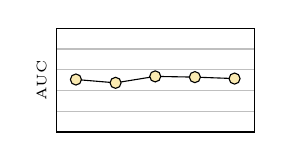
\begin{tikzpicture}
				\begin{axis}[
					height=2.9cm,
					width=4.1cm,
					xmajorticks=false,
					xmin=0.5,
					xmax=5.5,
					ymin=0,
					ymax=1,
					ylabel=\tiny{AUC},
					ymajorticks=false,
					ymajorgrids=true
				]
					\addplot[mark=*, draw=black, mark options={fill=baseline}] coordinates {
						(1, 0.506)
						(2, 0.474)
						(3, 0.536)
						(4, 0.529)
						(5, 0.515)
					};
				\end{axis}
			\end{tikzpicture}
		}
		\begin{tikzpicture}
			\begin{axis}[
				height=0.6\textwidth,
				width=0.8\textwidth,
				xlabel={Age},
				ylabel={Cognitive function},
				ticks=none,
				axis x line=bottom,
				axis y line=left,
				y axis line style={-|},
				xmin=0,
				xmax=1.4,
				ymin=0,
				ymax=1,
				clip=false
			]
			\addplot[draw=healthy-default, smooth, line width=4pt, opacity=0.5] coordinates {
				(0, 0.9)
				(0.25, 0.87)
				(0.5, 0.77)
				(0.6, 0.72)
				(0.8, 0.63)
				(0.9, 0.72)
				(1.4, 0.67)
			};
			\addplot[draw=controls-default, smooth, line width=4pt, opacity=0.5] coordinates {
				(0, 0.9)
				(0.25, 0.87)
				(0.5, 0.77)
				(0.6, 0.72)
				(0.8, 0.63)
				(0.9, 0.61)
				(1.4, 0.54)
			};
			\addplot[draw=cases-default, smooth, line width=4pt, opacity=0.5] coordinates {
				(0, 0.9)
				(0.25, 0.87)
				(0.5, 0.77)
				(0.6, 0.72)
				(0.8, 0.625)
				(1.1, 0.48)
				(1.4, 0.3)
			};
			\addplot[dashed] coordinates {
				(0, 0.65)
				(1.4, 0.65)
			};
			\addplot[dashed] coordinates {
				(0, 0.4)
				(1.4, 0.4)
			};
			\node[anchor=south west] at (axis cs: 0.1, 0.64) {\scriptsize{Normal cognition}};
			\node[anchor=north west] at (axis cs: 0.1, 0.66) {\scriptsize{Mild cognitive impairment}};
			\node[anchor=north west] at (axis cs: 0.1, 0.41) {\scriptsize{Dementia}};
			\node[anchor=west] at (axis cs: 1.4, 0.67) {\textcolor{healthy-default}{\footnotesize{Improving}}};
			\node[anchor=west] at (axis cs: 1.4, 0.53) {\textcolor{controls-default}{\footnotesize{Stable}}};
			\node[anchor=west] at (axis cs: 1.4, 0.3) {\textcolor{cases-default}{\footnotesize{Progressive}}};
			\draw[-stealth, red, thick] (axis cs: 0.8, 0.8) -- (axis cs: 0.8, 0.67);
			\node[anchor=south] at (axis cs: 0.8, 0.8) {\textcolor{red}{\footnotesize{t}}};
			\draw[densely dotted] (axis cs: 0.9, 0.8) -- (axis cs: 0.9, 0.3);
			\draw[densely dotted] (axis cs: 1, 0.8) -- (axis cs: 1, 0.3);
			\draw[densely dotted] (axis cs: 1.1, 0.8) -- (axis cs: 1.1, 0.3);
			\draw[densely dotted] (axis cs: 1.2, 0.8) -- (axis cs: 1.2, 0.3);
			\draw[densely dotted] (axis cs: 1.3, 0.8) -- (axis cs: 1.3, 0.3);
			\node[anchor=south] at (axis cs: 0.9, 0.8) {\footnotesize{t+1}};
			\node[anchor=south] at (axis cs: 1, 0.8) {\footnotesize{t+2}};
			\node[anchor=south] at (axis cs: 1.1, 0.8) {\footnotesize{t+3}};
			\node[anchor=south] at (axis cs: 1.2, 0.8) {\footnotesize{t+4}};
			\node[anchor=south] at (axis cs: 1.3, 0.8) {\footnotesize{t+5}};
			\node[] at (axis cs: 1.0755, 0.155) {
				\usebox{\resultsboxtwo}
			};
			\node[anchor=west] at (axis cs: 1.34, 0.158) {\footnotesize{0.51}};
			\end{axis}
		\end{tikzpicture}
		\vfill
	\end{frame}

	\begin{frame}{Mild cognitive impairment: Prognosis} % Prognosis
		\centering
		\vfill
		\newsavebox{\resultsboxone}
			\sbox{\resultsboxone}{%
			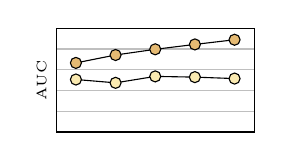
\begin{tikzpicture}
				\begin{axis}[
					height=2.9cm,
					width=4.1cm,
					xmajorticks=false,
					xmin=0.5,
					xmax=5.5,
					ymin=0,
					ymax=1,
					ylabel=\tiny{AUC},
					ymajorticks=false,
					ymajorgrids=true
				]
					\addplot[mark=*, draw=black, mark options={fill=baseline}] coordinates {
						(1, 0.506)
						(2, 0.474)
						(3, 0.536)
						(4, 0.529)
						(5, 0.515)
					};
					\addplot[mark=*, draw=black, mark options={fill=preds}] coordinates {
						(1, 0.666)
						(2, 0.742)
						(3, 0.797)
						(4, 0.844)
						(5, 0.889)
					};
				\end{axis}
			\end{tikzpicture}
		}
		\begin{tikzpicture}
			\begin{axis}[
				height=0.6\textwidth,
				width=0.8\textwidth,
				xlabel={Age},
				ylabel={Cognitive function},
				ticks=none,
				axis x line=bottom,
				axis y line=left,
				y axis line style={-|},
				xmin=0,
				xmax=1.4,
				ymin=0,
				ymax=1,
				clip=false
			]
			\addplot[draw=healthy-default, smooth, line width=4pt, opacity=0.5] coordinates {
				(0, 0.9)
				(0.25, 0.87)
				(0.5, 0.77)
				(0.6, 0.72)
				(0.8, 0.63)
				(0.9, 0.72)
				(1.4, 0.67)
			};
			\addplot[draw=controls-default, smooth, line width=4pt, opacity=0.5] coordinates {
				(0, 0.9)
				(0.25, 0.87)
				(0.5, 0.77)
				(0.6, 0.72)
				(0.8, 0.63)
				(0.9, 0.61)
				(1.4, 0.54)
			};
			\addplot[draw=cases-default, smooth, line width=4pt, opacity=0.5] coordinates {
				(0, 0.9)
				(0.25, 0.87)
				(0.5, 0.77)
				(0.6, 0.72)
				(0.8, 0.625)
				(1.1, 0.48)
				(1.4, 0.3)
			};
			\addplot[dashed] coordinates {
				(0, 0.65)
				(1.4, 0.65)
			};
			\addplot[dashed] coordinates {
				(0, 0.4)
				(1.4, 0.4)
			};
			\node[anchor=south west] at (axis cs: 0.1, 0.64) {\scriptsize{Normal cognition}};
			\node[anchor=north west] at (axis cs: 0.1, 0.66) {\scriptsize{Mild cognitive impairment}};
			\node[anchor=north west] at (axis cs: 0.1, 0.41) {\scriptsize{Dementia}};
			\node[anchor=west] at (axis cs: 1.4, 0.67) {\textcolor{healthy-default}{\footnotesize{Improving}}};
			\node[anchor=west] at (axis cs: 1.4, 0.53) {\textcolor{controls-default}{\footnotesize{Stable}}};
			\node[anchor=west] at (axis cs: 1.4, 0.3) {\textcolor{cases-default}{\footnotesize{Progressive}}};
			\draw[-stealth, red, thick] (axis cs: 0.8, 0.8) -- (axis cs: 0.8, 0.67);
			\node[anchor=south] at (axis cs: 0.8, 0.8) {\textcolor{red}{\footnotesize{t}}};
			\draw[densely dotted] (axis cs: 0.9, 0.8) -- (axis cs: 0.9, 0.3);
			\draw[densely dotted] (axis cs: 1, 0.8) -- (axis cs: 1, 0.3);
			\draw[densely dotted] (axis cs: 1.1, 0.8) -- (axis cs: 1.1, 0.3);
			\draw[densely dotted] (axis cs: 1.2, 0.8) -- (axis cs: 1.2, 0.3);
			\draw[densely dotted] (axis cs: 1.3, 0.8) -- (axis cs: 1.3, 0.3);
			\node[anchor=south] at (axis cs: 0.9, 0.8) {\footnotesize{t+1}};
			\node[anchor=south] at (axis cs: 1, 0.8) {\footnotesize{t+2}};
			\node[anchor=south] at (axis cs: 1.1, 0.8) {\footnotesize{t+3}};
			\node[anchor=south] at (axis cs: 1.2, 0.8) {\footnotesize{t+4}};
			\node[anchor=south] at (axis cs: 1.3, 0.8) {\footnotesize{t+5}};
			\node[] at (axis cs: 1.0755, 0.155) {
				\usebox{\resultsboxone}
			};
			\node[anchor=west] at (axis cs: 1.34, 0.261) {\footnotesize{0.88}};
			\end{axis}
		\end{tikzpicture}
		\vfill
	\end{frame}

	\begin{frame}{Mild cognitive impairment: Prognosis} % Prognosis
		\centering
		\vfill
		\newsavebox{\resultsbox}
			\sbox{\resultsbox}{%
			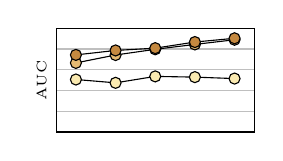
\begin{tikzpicture}
				\begin{axis}[
					height=2.9cm,
					width=4.1cm,
					xmajorticks=false,
					xmin=0.5,
					xmax=5.5,
					ymin=0,
					ymax=1,
					ylabel=\tiny{AUC},
					ymajorticks=false,
					ymajorgrids=true
				]
					\addplot[mark=*, draw=black, mark options={fill=baseline}] coordinates {
						(1, 0.506)
						(2, 0.474)
						(3, 0.536)
						(4, 0.529)
						(5, 0.515)
					};
					\addplot[mark=*, draw=black, mark options={fill=preds}] coordinates {
						(1, 0.666)
						(2, 0.742)
						(3, 0.797)
						(4, 0.844)
						(5, 0.889)
					};
					\addplot[mark=*, draw=black, mark options={fill=maps}] coordinates {
						(1, 0.743)
						(2, 0.786)
						(3, 0.808)
						(4, 0.867)
						(5, 0.903)
					};
				\end{axis}
			\end{tikzpicture}
		}
		\begin{tikzpicture}
			\begin{axis}[
				height=0.6\textwidth,
				width=0.8\textwidth,
				xlabel={Age},
				ylabel={Cognitive function},
				ticks=none,
				axis x line=bottom,
				axis y line=left,
				y axis line style={-|},
				xmin=0,
				xmax=1.4,
				ymin=0,
				ymax=1,
				clip=false
			]
			\addplot[draw=healthy-default, smooth, line width=4pt, opacity=0.5] coordinates {
				(0, 0.9)
				(0.25, 0.87)
				(0.5, 0.77)
				(0.6, 0.72)
				(0.8, 0.63)
				(0.9, 0.72)
				(1.4, 0.67)
			};
			\addplot[draw=controls-default, smooth, line width=4pt, opacity=0.5] coordinates {
				(0, 0.9)
				(0.25, 0.87)
				(0.5, 0.77)
				(0.6, 0.72)
				(0.8, 0.63)
				(0.9, 0.61)
				(1.4, 0.54)
			};
			\addplot[draw=cases-default, smooth, line width=4pt, opacity=0.5] coordinates {
				(0, 0.9)
				(0.25, 0.87)
				(0.5, 0.77)
				(0.6, 0.72)
				(0.8, 0.625)
				(1.1, 0.48)
				(1.4, 0.3)
			};
			\addplot[dashed] coordinates {
				(0, 0.65)
				(1.4, 0.65)
			};
			\addplot[dashed] coordinates {
				(0, 0.4)
				(1.4, 0.4)
			};
			\node[anchor=south west] at (axis cs: 0.1, 0.64) {\scriptsize{Normal cognition}};
			\node[anchor=north west] at (axis cs: 0.1, 0.66) {\scriptsize{Mild cognitive impairment}};
			\node[anchor=north west] at (axis cs: 0.1, 0.41) {\scriptsize{Dementia}};
			\node[anchor=west] at (axis cs: 1.4, 0.67) {\textcolor{healthy-default}{\footnotesize{Improving}}};
			\node[anchor=west] at (axis cs: 1.4, 0.53) {\textcolor{controls-default}{\footnotesize{Stable}}};
			\node[anchor=west] at (axis cs: 1.4, 0.3) {\textcolor{cases-default}{\footnotesize{Progressive}}};
			\draw[-stealth, red, thick] (axis cs: 0.8, 0.8) -- (axis cs: 0.8, 0.67);
			\node[anchor=south] at (axis cs: 0.8, 0.8) {\textcolor{red}{\footnotesize{t}}};
			\draw[densely dotted] (axis cs: 0.9, 0.8) -- (axis cs: 0.9, 0.3);
			\draw[densely dotted] (axis cs: 1, 0.8) -- (axis cs: 1, 0.3);
			\draw[densely dotted] (axis cs: 1.1, 0.8) -- (axis cs: 1.1, 0.3);
			\draw[densely dotted] (axis cs: 1.2, 0.8) -- (axis cs: 1.2, 0.3);
			\draw[densely dotted] (axis cs: 1.3, 0.8) -- (axis cs: 1.3, 0.3);
			\node[anchor=south] at (axis cs: 0.9, 0.8) {\footnotesize{t+1}};
			\node[anchor=south] at (axis cs: 1, 0.8) {\footnotesize{t+2}};
			\node[anchor=south] at (axis cs: 1.1, 0.8) {\footnotesize{t+3}};
			\node[anchor=south] at (axis cs: 1.2, 0.8) {\footnotesize{t+4}};
			\node[anchor=south] at (axis cs: 1.3, 0.8) {\footnotesize{t+5}};
			\node[] at (axis cs: 1.0755, 0.155) {
				\usebox{\resultsbox}
			};
			\node[anchor=west] at (axis cs: 1.34, 0.262) {\footnotesize{0.90}};
			\end{axis}
		\end{tikzpicture}
		\vfill
	\end{frame}

	\begin{frame}{Mild cognitive impairment: Correlation with cognitive scores} % Correlations
		\newcommand{\mriwidth}{2.2cm}
        \newcommand{\gap}{0.00cm}

        \newcommand{\correlationplot}[4]{
            \begin{tikzpicture}
                \begin{axis}[
                    height=1.71 * \mriwidth,
                    width=1.71 * \mriwidth,
                    xmajorticks=false,
                    ylabel=####3,
                    ytick={0, 2, 4, 6, 8},
                    yticklabels=####2,
                    xmin=-1,
                    xmax=17,
                    ymin=0,
                    ymax=9,
                    every tick label/.append style={font=\tiny},
                    ytick pos=left,
                    scatter/classes={
                        ADNI_EF={color0, draw=black},
                        ADNI_MEM={color1, draw=black},
                        CDCARE={color2, draw=black},
                        CDCOMMUN={color3, draw=black},
                        CDGLOBAL={color4, draw=black},
                        CDHOME={color5, draw=black},
                        CDJUDGE={color6, draw=black},
                        CDMEMORY={color7, draw=black},
                        CDORIENT={color8, draw=black},
                        FAQTOTAL={color9, draw=black},
                        GDTOTAL={color10, draw=black},
                        MMSCORE={color11, draw=black},
                        NPISCORE={color12, draw=black},
                        PHC_EXF={color13, draw=black},
                        PHC_LAN={color14, draw=black},
                        PHC_MEM={color15, draw=black},
                        PHC_VSP={color16, draw=black}
                    },
                    y label style={at={(-0.1,0.5)}},
                    ymajorgrids=true,
                    ytick style={draw=none},
                    clip=false,
                    grid style={draw=gray!20},
                    axis line style={draw=gray!70}
                ]
                    \addplot[
                        only marks,
                        scatter,
                        scatter src=explicit symbolic
                    ] table [
                        col sep=comma,
                        x=index,
                        y=component_####1,
                        meta=symptom
                    ] {data/correlations.csv};
                    \addplot[dashed,red, thick] coordinates {
                        (-1, 2.76)
                        (17, 2.76)
                    };
                    ####4
                \end{axis}
            \end{tikzpicture}
        }

        \newsavebox{\firstcorrelations}
        \sbox{\firstcorrelations}{%
            \correlationplot{0}{{0, 2, 4, 6, 8}}{\scriptsize{$-log_{10}(p)$}}{
                \node[] at (axis cs: 14, 6.09) {\tiny{PHC\_LAN}};
            }
        }
        \newsavebox{\secondcorrelations}
        \sbox{\secondcorrelations}{%
            \correlationplot{1}{{,,}}{{}}{
                \node[] at (axis cs: 9, 3.64) {\tiny{FAQTOTAL}};
            }
        }
        \newsavebox{\thirdcorrelations}
        \sbox{\thirdcorrelations}{%
            \correlationplot{2}{{,,}}{{}}{
                \node[] at (axis cs: 0, 6.34) {\tiny{ADNI\_EF}};
                \node[] at (axis cs: 13, 7.85) {\tiny{PHC\_EXF}};
            }
        }
        \newsavebox{\fourthcorrelations}
        \sbox{\fourthcorrelations}{%
            \correlationplot{3}{{,,}}{{}}{
                \node[] at (axis cs: 0, 8.92) {\tiny{ADNI\_EF}};
                \node[] at (axis cs: 13, 8.65) {\tiny{PHC\_EXF}};
                \node[] at (axis cs: 14, 5.84) {\tiny{PHC\_LAN}};
                \node[] at (axis cs: 6, 5.08) {\tiny{CDJUDGE}};
                \node[] at (axis cs: 11, 3.89) {\tiny{MMSCORE}};
            }
        }

        \begin{tikzpicture}
            \node[] (first) at (0, 0) {
                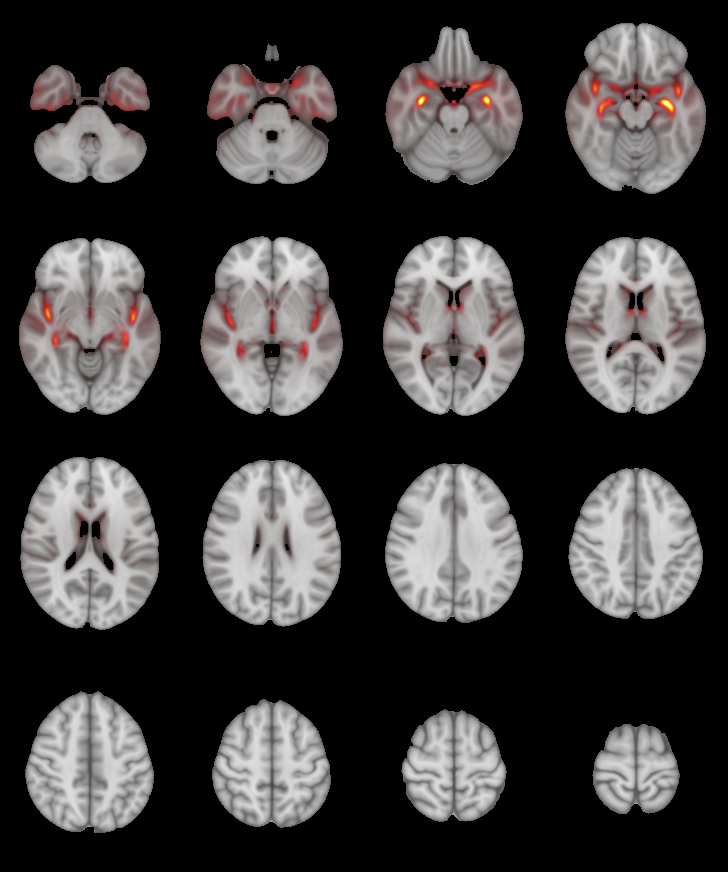
\includegraphics[
                    width=\mriwidth,
                    clip=true,
                    trim = 192mm 232mm 0mm 0mm
                ]{data/components/component_0.png}
            };
            \node[anchor=north west] (first-correlation) at ($ (first.south west) + (-0.73, 0.1) $) {
                \usebox{\firstcorrelations}
            };

            \node[anchor=west] (second) at ($ (first.east) + (\gap, 0) $) {
                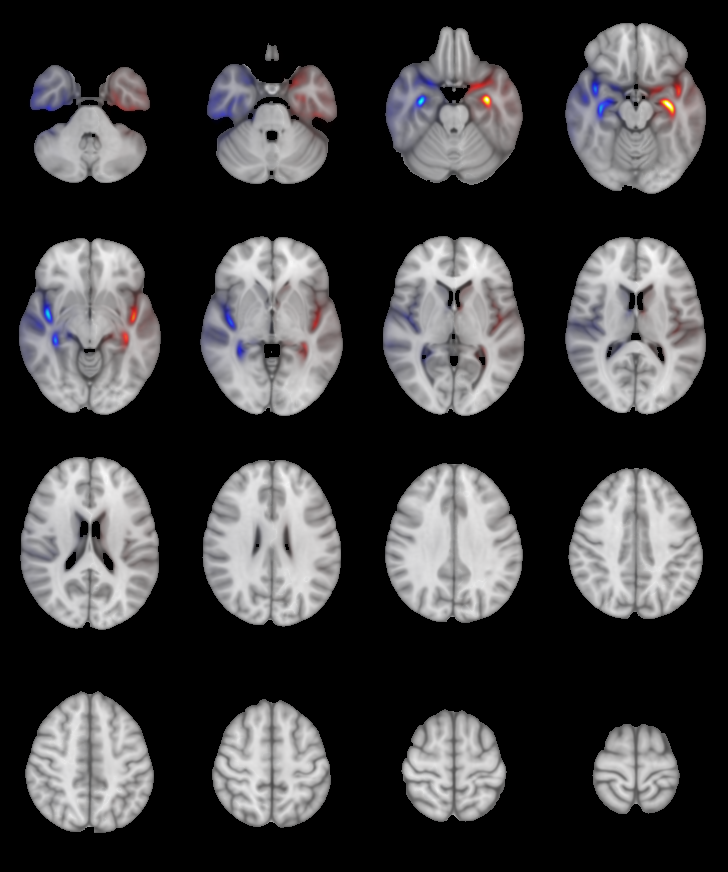
\includegraphics[
                    width=\mriwidth,
                    clip=true,
                    trim = 192mm 232mm 0mm 0mm
                ]{data/components/component_1.png}
            };
            \node[anchor=north west] (second-correlation) at ($ (first-correlation.north east) - (0.56, 0) $) {
                \usebox{\secondcorrelations}
            };

            \node[anchor=west] (third) at ($ (second.east) + (\gap, 0) $) {
                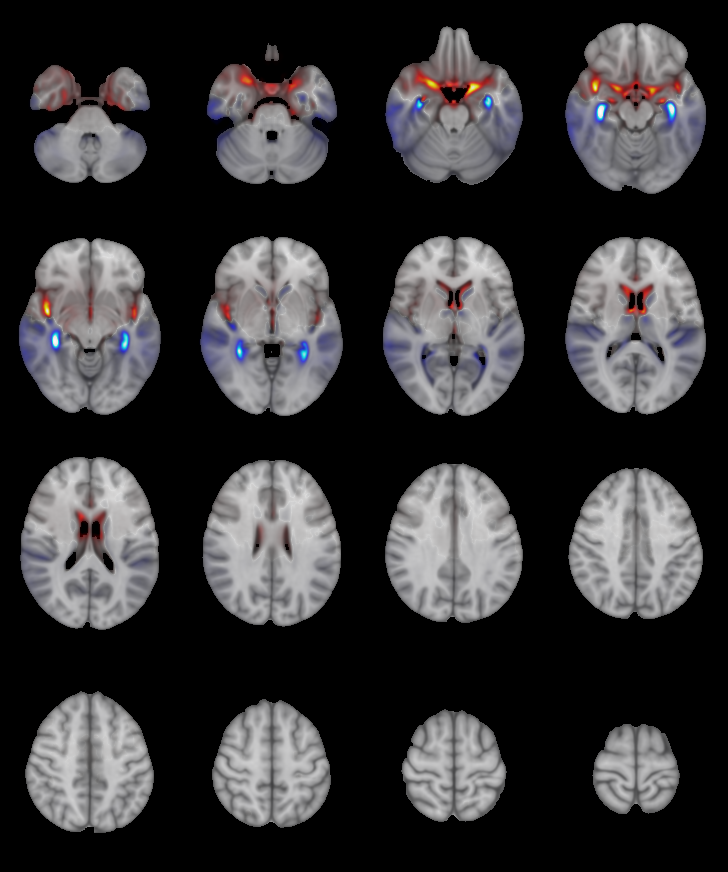
\includegraphics[
                    width=\mriwidth,
                    clip=true,
                    trim = 192mm 232mm 0mm 0mm
                ]{data/components/component_2.png}
            };
            \node[anchor=north west] (third-correlation) at ($ (second-correlation.north east) - (0.56, 0) $) {
                \usebox{\thirdcorrelations}
            };

            \node[anchor=west] (fourth) at ($ (third.east) + (\gap, 0) $) {
                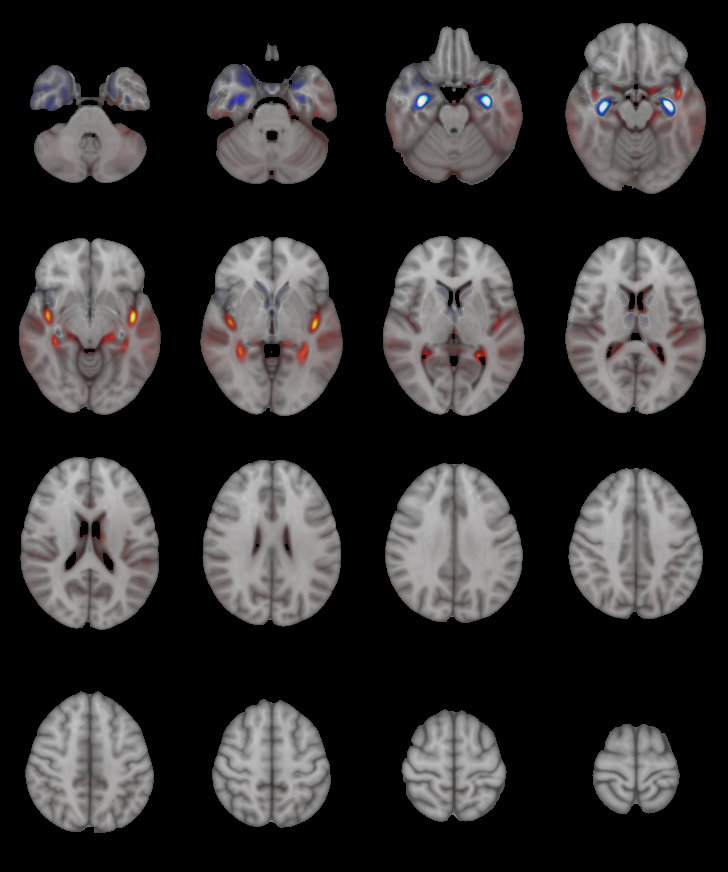
\includegraphics[
                    width=\mriwidth,
                    clip=true,
                    trim = 192mm 232mm 0mm 0mm
                ]{data/components/component_3.png}
            };
            \node[anchor=north west] (fourth-correlation) at ($ (third-correlation.north east) - (0.56, -0.16) $) {
                \usebox{\fourthcorrelations}
            };
        \end{tikzpicture}
	\end{frame}

	\begin{frame}{Mild cognitive impairment: Morphological record}
		\centering
		\colorlet{ninety}{cases-default}
		\colorlet{fifty}{controls-default}
		\colorlet{ten}{healthy-default}

		\newcommand{\mriwidth}{2.59cm}
		\newcommand{\gap}{0.00cm}

		\newsavebox{\survival}
		\sbox{\survival}{%
			\begin{tikzpicture}
				\begin{axis}[
					height=2.5cm,
					width=3.5cm,
					every tick label/.append style={font=\tiny},
					xtick pos=bottom,
					ytick={0, 0.2, 0.4, 0.6, 0.8, 1.0},
					ymin=0,
					ymax=1,
					xmin=62,
					xmax=95,
					ytick pos=right,
					ytick style={draw=none},
					ymajorgrids=true,
					grid style={line width=.5pt, draw=gray!25},
				]

				\addplot[gray, very thick] table [col sep=comma, x=age, y=baseline] {data/subject_survival.csv};
				\addplot[cases-default, very thick] table [col sep=comma, x=age, y=subject] {data/subject_survival.csv};
				\addplot[cases-default, only marks, draw=black] coordinates {(66, 0.98)};

				\end{axis}
			\end{tikzpicture}
			}
		\begin{tikzpicture}[scale=0.75]

			\def\xmin{1.15}
			\def\xmax{10.99}
			\def\ymin{-3.5}
			\def\ymax{-0.5}
			\def\xstep{0.492}
			\node[draw=none,anchor=north west] at (0, 0) {};
			\node[draw=none,anchor=south east] at (12.14, -5){};

			\colorlet{faded-black}{black!30}
			\colorlet{faded-white}{white!30}
			\colorlet{faded-cases}{cases-default!30}

			\draw[black] (\xmin, \ymax) -- (\xmax, \ymax) -- (\xmax, \ymin) -- (\xmin, \ymin) -- (\xmin, \ymax);
			\node[anchor=east] at (\xmin, -0.5) {\footnotesize{1.0}};
			\node[anchor=east] at (\xmin, -1.1) {\footnotesize{0.8}};
			\node[anchor=east] at (\xmin, -1.7) {\footnotesize{0.6}};
			\node[anchor=east] at (\xmin, -2.3) {\footnotesize{0.4}};
			\node[anchor=east] at (\xmin, -2.9) {\footnotesize{0.2}};
			\node[anchor=east] at (\xmin, -3.5) {\footnotesize{0.0}};
			\node[rotate=90,anchor=south] at ($ (\xmin, -2) - (0.7, 0) $) {\footnotesize{Dementia prediction}};

			\draw[gray!50, thin] (\xmin, -1.1) -- (\xmax, -1.1);
			\draw[gray!50, thin] (\xmin, -1.7) -- (\xmax, -1.7);
			\draw[gray!50, thin] (\xmin, -2.3) -- (\xmax, -2.3);
			\draw[gray!50, thin] (\xmin, -2.9) -- (\xmax, -2.9);

			\draw[dashed] (\xmin + 3.99 * \xstep, \ymin) -- (\xmin + 3.99 * \xstep, \ymax);

			\newcommand{\prediction}[5]{
				\node[circle, inner sep=0pt, outer sep=0pt, minimum size=6pt, draw=####5, fill=####3] (####4) at (\xmin + ####1 * \xstep, \ymin+3*####2) {};
			}

			\prediction{1}{0.5369713}{controls-default}{p1}{black}
			\prediction{3}{0.5685464}{controls-default}{p2}{black}
			\prediction{5}{0.72608125}{faded-cases}{p3}{faded-black}
			\prediction{7}{0.7650767}{faded-cases}{p4}{faded-black}
			\prediction{9}{0.78441274}{faded-cases}{p5}{faded-black}
			\prediction{11}{0.77807206}{faded-cases}{p6}{faded-black}
			\prediction{13}{0.96812713}{faded-cases}{p7}{faded-black}
			\prediction{15}{0.9813527}{faded-cases}{p8}{faded-black}
			\prediction{17}{0.99700356}{faded-cases}{p9}{faded-black}
			\prediction{19}{0.998078}{faded-cases}{p10}{faded-black}

			\node[anchor=north] at (\xmin + 3.1 * \xstep, \ymin + 3 * 0.5585) {\scriptsize{$0.57$}};
			\node[anchor=south, rotate=6] at (\xmin + 2 * \xstep, \ymin + 3 * 0.542) {\scriptsize{$\angle 0.05$}};

			\draw[controls-default, thick] (p1) -- (p2);
			\draw[faded-cases, thick] (p2) -- (p3) -- (p4) -- (p5) -- (p6) -- (p7) -- (p8) -- (p9) -- (p10);

			\node[anchor=north, inner sep=0pt, outer sep=0pt] (masks) at (\xmin + 10*\xstep+0.001 + 0.002, \ymin) {
				{\transparent{0.3}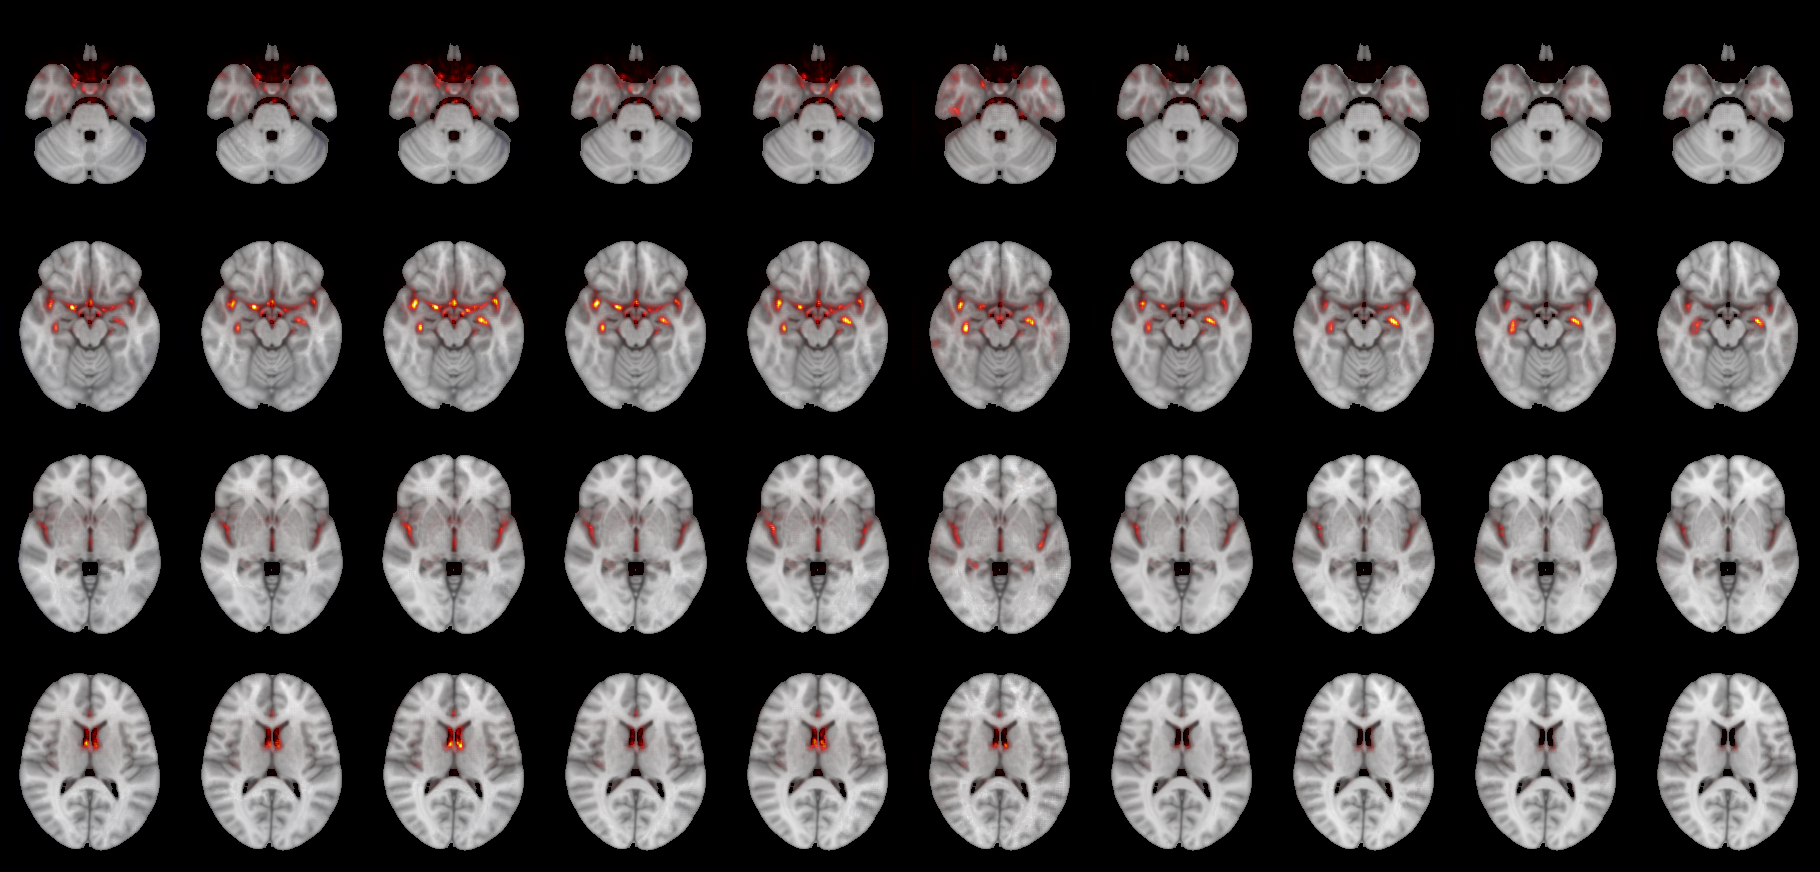
\includegraphics[width=0.684\textwidth]{data/MCI_to_AD.png}}
			};

			% Opaque images
			\node[anchor=north west, inner sep=0pt, outer sep=0pt] at ($ (masks.north west) + (-0.008, 0) $) {
				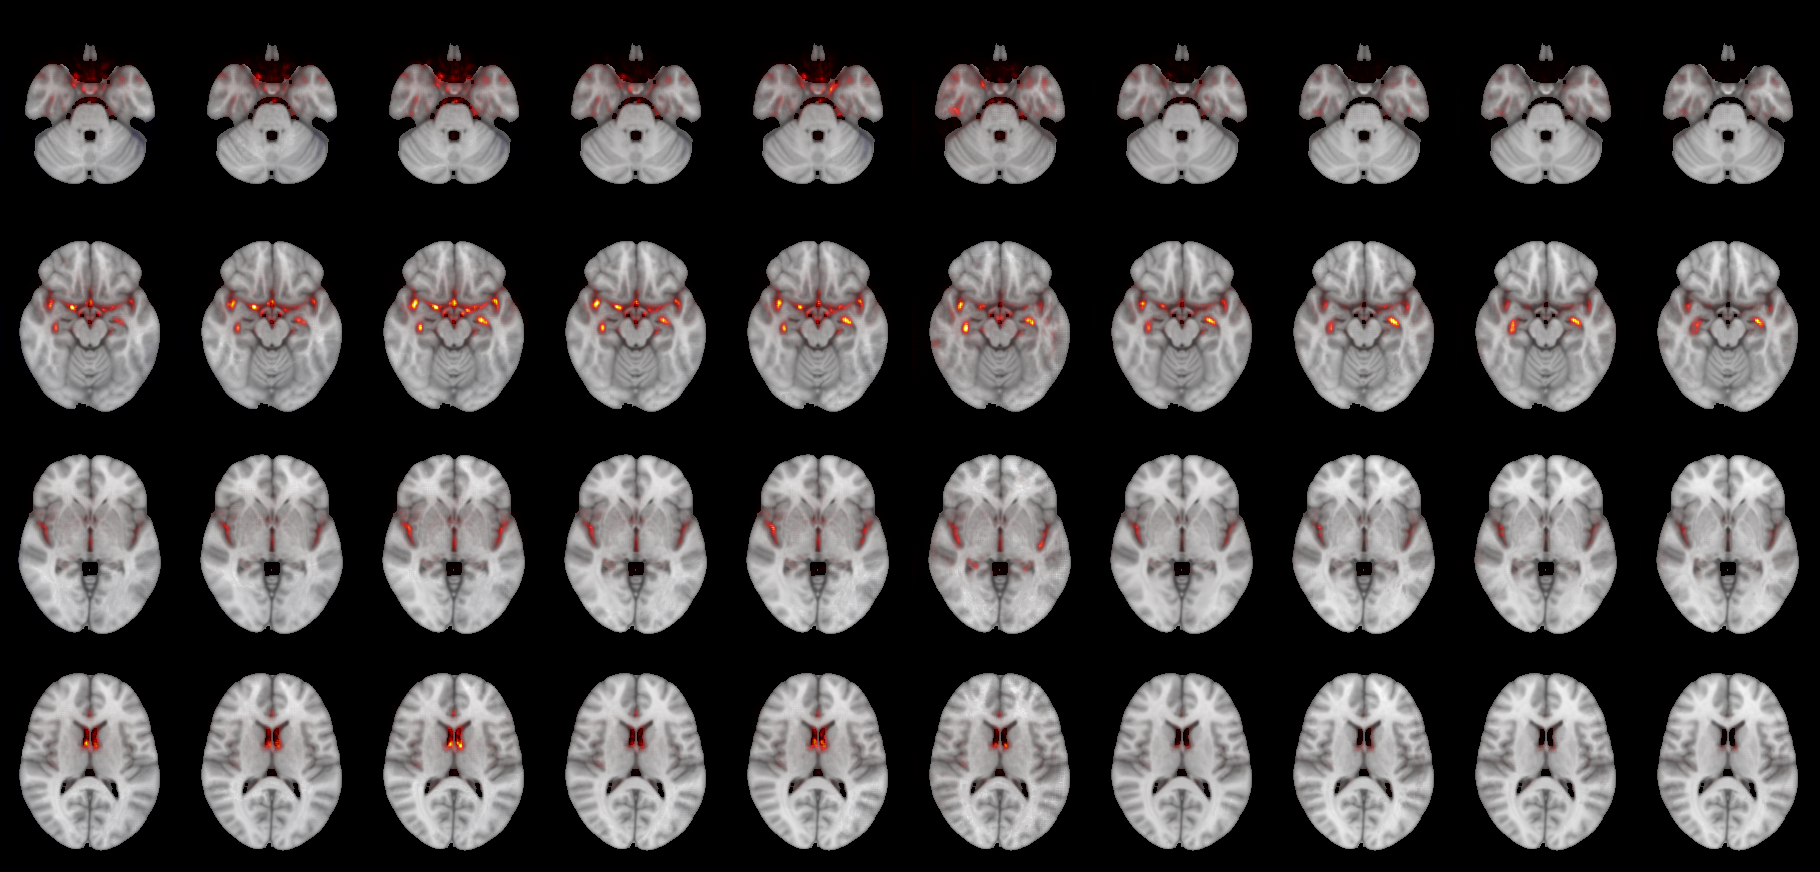
\includegraphics[
					width=0.1362\textwidth,
					trim={0cm 0cm 51.42cm 0cm},
					clip=true
				]{data/MCI_to_AD.png}
			};

			\newcommand{\datenode}[4]{
				\node[fill=####3,inner sep=0pt,anchor=north,font=\tiny\selectfont] at ($ (\xmin, \ymin) + (####2 * \xstep, -0.1) $) {\textcolor{####4}{####1}};
			}

			\datenode{17.07.06}{1}{black}{white}
			\datenode{22.02.07}{3}{black}{white}
			\datenode{05.09.07}{5}{faded-black}{faded-white}
			\datenode{03.04.08}{7}{faded-black}{faded-white}
			\datenode{29.09.08}{9}{faded-black}{faded-white}
			\datenode{13.08.09}{11}{faded-black}{faded-white}
			\datenode{22.07.10}{13}{faded-black}{faded-white}
			\datenode{16.08.11}{15}{faded-black}{faded-white}
			\datenode{07.08.12}{17}{faded-black}{faded-white}
			\datenode{16.08.13}{19}{faded-black}{faded-white}

			\node[] at (\xmin + 7 * \xstep, \ymax + 0.2) {\footnotesize{$72.41\%$}};
			\node[] at (\xmin + 11 * \xstep, \ymax + 0.2) {\footnotesize{$81.17\%$}};
			\node[] at (\xmin + 15 * \xstep, \ymax + 0.2) {\footnotesize{$89.96\%$}};
			\node[] at (\xmin + 19 * \xstep, \ymax + 0.2) {\footnotesize{$94.89\%$}};
			\node[] at (\xmin + 13 * \xstep, \ymax + 0.6) {\textbf{\footnotesize{\textit{Predicted probability of progression}}}};

			\node[anchor=south, text depth=0] (mcitext) at (\xmin + 8.47 * \xstep, \ymin + 3 * 0.02) {\footnotesize{MCI}};
			\node[
				anchor=east,
				circle,
				inner sep=0pt,
				outer sep=0pt,
				minimum size=6pt,
				draw=black,
				fill=controls-default
			] (mcidot) at (mcitext.west) {};
			\node[
				anchor=west,
				circle,
				inner sep=0pt,
				outer sep=0pt,
				minimum size=6pt,
				draw=faded-black,
				fill=faded-cases
			] (dementiadot) at ($ (mcitext.east) + (0.1, 0) $) {};
			\node[anchor=west, text depth=0] at (dementiadot.east) {\textcolor{faded-black}{\footnotesize{Dementia}}};

			\node[anchor=north] (survivalnode) at (\xmin + 2.7 * \xstep, \ymin - 2.7 * 1.7) {
				\usebox{\survival}
			};

			\node[] (averagetext) at ($ (survivalnode.south) + (-0.15, 0) $) {\scriptsize{Average}};
			\draw[gray, very thick] (averagetext.west) -- ($ (averagetext.west) - (0.25, 0) $);
			\draw[cases-default, very thick] ($ (averagetext.west) - (0, 0.3) $) -- ($ (averagetext.west) - (0.25, 0.3) $);
			\node[] at ($ (averagetext) - (0, 0.3) $) {\scriptsize{Patient}};

			\node[
				anchor=north west,
			] (header) at ($ (survivalnode.north east) + (0.6, -0.12) $) {
				\footnotesize{\textbf{\textit{Expected cognitive deviations:}}}
			};
			\node[
				anchor=north west,
				font=\footnotesize\linespread{0.85}\selectfont,
				align=left,
			] at ($ (header.south west)  + (0, 0.1)$) {
				\bullet\hspace{0.05cm} \textit{The patient is predicted to have}\\
				\textit{impaired executive function.}
			};

			\node[anchor=south east, text depth=0] at (\xmin + 4 * \xstep, \ymax - 0.2 * 3) {\Large{\textbf{a}}};
			\node[anchor=south west, text depth=0] at (\xmin + 4 * \xstep, \ymax - 0.2 * 3) {\Large{\textbf{b}}};
			\node[text depth=0] at (\xmin + 7.1 * \xstep, \ymax + 0.26 * 3) {\Large{\textbf{c}}};
			\node[anchor=north east, text depth=0] (d) at ($ (survivalnode.north west) + (0.1, -0.15) $) {\Large{\textbf{d}}};
			\node[anchor=south west, text depth=0] (d) at ($ (d.south east) + (3.6, 0) $) {\Large{\textbf{e}}};
		\end{tikzpicture}
	\end{frame}

	\begin{frame}{Future directions} % MS
	\centering
	\vfill
	\begin{tikzpicture}
		\node[draw=none] at (-2, -2) {};
		\node[draw=none] at (6.5, 2.5) {};
		\node[label={[text depth=0]above:Dementia}] at (0, 0) {
			
\includegraphics[width=0.31\textwidth]{data/dementia.png}
		};

		\node[label={[text depth=0]above:Multiple sclerosis}] at (4.5, 0) {
			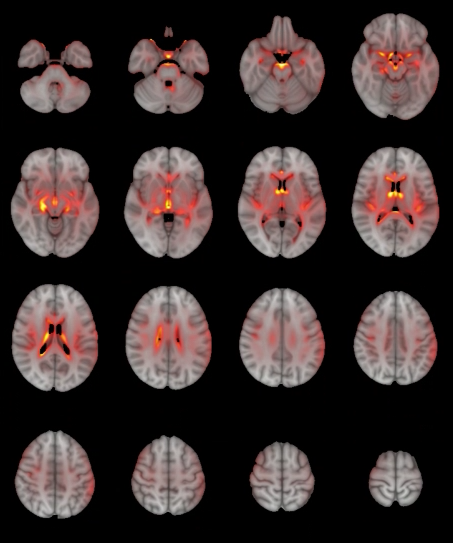
\includegraphics[width=0.31\textwidth]{data/ms.png}
		};
	\end{tikzpicture}
	\vfill
	\end{frame}
\end{document}
